\documentclass[a4paper,12pt]{article}
% a4paper sets it up with the measures for A4 paper
% 12pt is the lettering size, (you can use 11pt or 12pt)

% this produces A4 pages with a lot more text on each page
\usepackage{a4wide}
\usepackage{hyperref}
% this tells LaTeX how the latex file is encoded
% on a modern linux usually utf8, older linux in Sweden usually latin1
% Windows has sometimes, but not always, its own encoding
% latin1 and utf8 allow direct input of accented characters like åäö 
\usepackage[utf8]{inputenc}
\usepackage[table,xcdraw]{xcolor}
\usepackage{multirow}
% uncomment (i.e. remove the % in front) for a fancier bibliography
%\bibliographystyle{natbib}

% this defines the \includegraphics command used for including figures
\usepackage{graphicx}

\usepackage{pdfpages}
% the amsmath package has a lot of useful stuff for equations,
% especially for ligning up multiple equations
\usepackage{amsmath}


\begin{document}

%%%%%%%%%%%%%%%%%%%%%%%%%%%%%%%%%%%%%%%%%%%%%%%%%%%%%%%%%%%%%%%%%%%%%%%%%%%
% first as you might guess the title page
\begin{titlepage}
% flushright puts it towards the right of the page
%\begin{flushright}
% our preprint number yy-nn (year-number), ask your supervisor how to get this
%LU TP 14-nn\\
% some indication of the date
%June 2014\\
%\end{flushright}
\vfill
\begin{center}
% put in line breaks to make the title look nicer and provide more
% space between the lines
{\large\bf Zebrafish larva action sequence analysis.}
\\[3cm]
{\bf Jerneja Mislej}
\\[1.5cm]
{Master thesis supervised by Fredrik Ek\\and\\co-supervised by Mauno Vihinen}
\\[4cm]
% use the eps version for latex and the pdf version for pdflatex 

\includegraphics[height=4cm]{Lund_University_logotype.png}
\\[0.5cm]
{2017}
\\[2cm]
\end{center}
{Examensarbete för 30 hp\\
Institutionen för ?, ? fakulteten, Lunds universitet
\\
\\Thesis for a ? in ?, 30 ECTS credits
\\Department of ?, Faculty of ?, Lund University}

\end{titlepage}
%%%%%%%%%%%%%%%%%%%%%%%%%%%%%%%%%%%%%%%%%%%%%%%%%%%%%%%%%%%%%%%%%%%%%%%%%%%
% a page with the abstract and popular description
\thispagestyle{empty} % do not count pages just yet

% these 'rubber' spaces make the page layout look nicer
%the \phantom{p} is to make something there for the \vfill to push against

\section*{Abstract}
Zebrafish larvae action sequences are analysed in order to compare and profile several different drugs for therapeutic purposes in neurological diseases. Healthy and neurological disease induced larvae were treated with different drugs and drug dosages and their movement recorded into action sequences. Action sequences consist of eight different turn types, organised in swim bouts. Descriptive statistics, derived from bout length, bout frequency, distribution of turns and turn transitions, can be linked to the larval neurological state. By conducting exploratory data analysis, different drugs and drug dosages can be compared in their effect on the neurological state of healthy and disease induced larvae. Most influential descriptive statistics are examined further, by obtaining effect sizes with reference to the healthy larvae in a mixed effects model.
\phantom{p}
\vfill

\newpage

\tableofcontents
% the list of figures and tables is optional
\listoffigures 
\listoftables

\newpage

\section{Introduction}
Zebrafish(\textit{Danio rerio}) have become increasingly used as a model for human disease and pharmaceutical research\cite{ref1}-\cite{ref3}. 
\\In development of novel
clinical drugs, several prerequisites are necessary before human trial is possible. These prerequisites rely on evaluations of functionalities of entire basic
vital systems, like for example cardiac, central nervous or respiratory system\cite{ref4}.
Although novel and improved in-vitro methods are being developed, the need for a live animal model is currently still inevitable for many evaluations in pharmacology investigations and toxicology studies, where the majority of animal models rely on rodents. The use of zebrafish as an animal model has been established to improve and aid in drug trials depending on an animal model such as rats and mice.
Due to its fecundity, morphological and physiological similarity to mammals, the zebrafish animal model enables a more profound and accurate compound screening process. 
Particularly, the larval zebrafish model, since it combines the advantages of in-vitro high-throughput screening techniques and whole organism phenotype data. By improving the compound screening of
the drugs entering the trial, the gap between cell-based and whole mammal organism trials is reduced, thus optimising the entire further trial process and reducing the consumption
of rodents\cite{ref1}. \\Example in Figure 1.
\begin{figure}[h]
\begin{center}
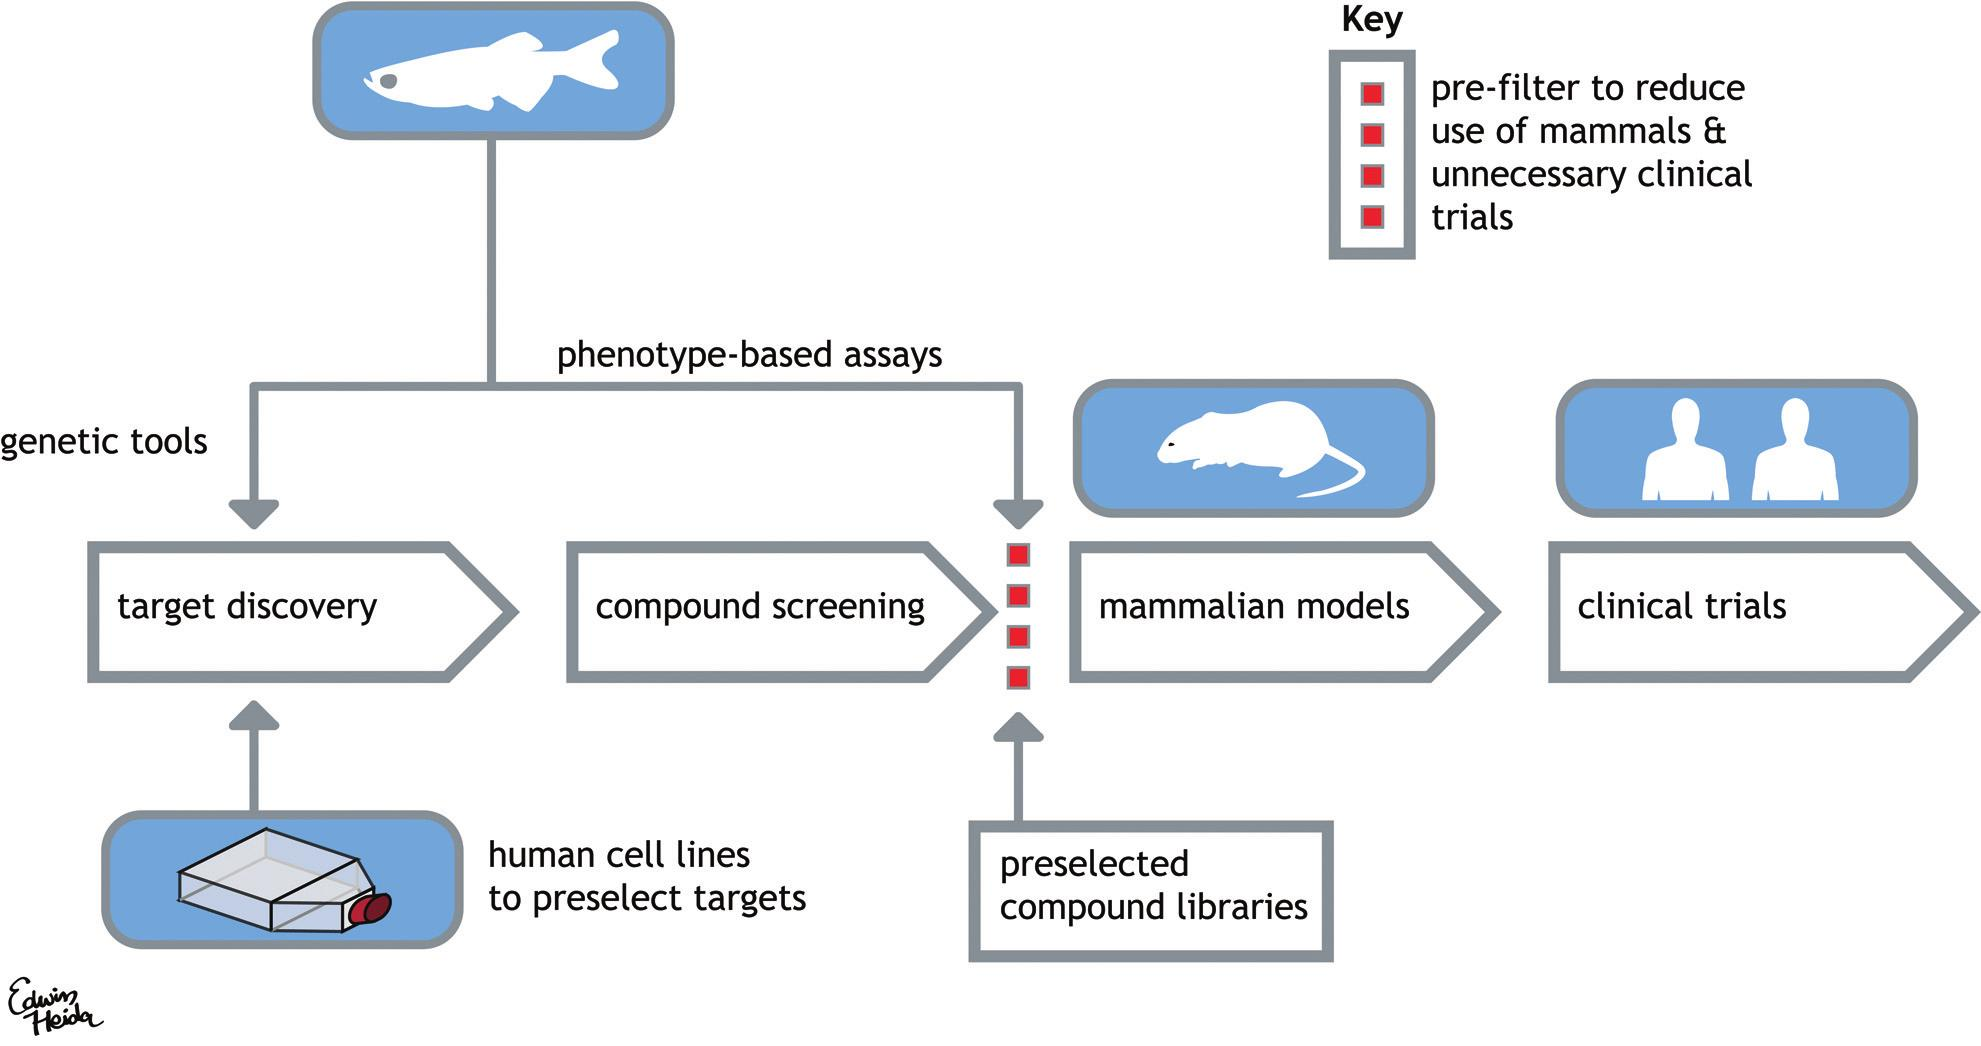
\includegraphics[width=15cm,height=7cm]{drug_trial_example.jpg}
\caption{Clinical drug development pipeline showing incorporation of zebrafish animal models. Graphics taken from article \textit{Zebrafish development and regeneration:
new tools for biomedical research} by Brittijn S.A. \textit{et al.}, published at \textcopyright 2009 UBC Press\cite{ref1}. }
\end{center}
\end{figure}
\\
Screening technologies based on zebrafish larvae have been and are still being developed for therapeutic purposes across a wide range of diseases, such as cancer, cardiovascular, metabolic and neurological diseases in particular\cite{ref5}-\cite{ref8}. \\Zebrafish larvae display predation, fear, stress, exploration, drug addiction, and other neurobehavioral phenotypes that are quantifiable and relate to those seen in humans and are therefore suitable for neurobehavioural profiling of potential medication of neurological diseases\cite{ref9}\cite{ref10}. Target and off-target effects of potential medications can be tested, by analysing larvae movement under conditions known to cause abnormal neurological behaviour, like for example excesive stress and hyper or hypo activity\cite{ref11}-\cite{ref16}.
\\Zebrafish larvae are more comfortable in the dark as they feel less exposed to predators and thus feel safer, while constant exposure to light induces stress-like behaviour\cite{ref16}. \\Several chemical compounds have also been shown to lead to neurobehavioral changes. 
For example, Apomorphine used to treat neurological diseases like schizofrenia\cite{ref12} and Parkinson's disease\cite{ref11}, will, if administered in low doses, induce a hypoactive or a sedated state, while a high dose of Apomorphine induces a hyperactive or a stressed state\cite{ref13}. Hyperactive/stressed state can also be induced with a sub-convulsive concentrations of pentylenetetrazol(PTZ)\cite{ref14}. A wide range of commerical drugs and novel chemical compounds have already been profiled in their effects on the neurological state induced by Apomorphine or PTZ\cite{ref13}\cite{ref15}. Potential novel drugs can, therefore, be profiled according to their similarity to known profiles of drugs with known target and off-target effects.\\By analysing zebrafish larvae behaviour and locomotion phenotypes, corresponding phenotypical changes can be linked to the drugs administered along with Apomorphine or PTZ. General behaviour phenotypes in zebrafish include place preference, social interaction, cognitive performance etc, while locomotion phenotypes include the length and frequency of swimming bouts and types of turns performed in the movement\cite{ref17}\cite{ref18}. \\Several turn types have been distinguished by the subsequent turn angles at a certain velocity and have been shown to represent zebrafish predation, startle and normal/routine behaviour\cite{ref9}. For example, startle/escape is represented by a high-velocity turn, where the zebrafish performs a C-shaped bend in the opposite direction, followed by a less powerful counterturn and a vigorous swimming episode(burst swim), an example in Figure 2. This behaviour has been linked to the central nervous system(CNS), particularly to the Mauthner neuron\cite{ref19}. Deviations from a typical zebrafish startle/escape locomotion pattern have been linked to disorders in the neural network involving Mauthner neurons\cite{ref20}.
\begin{figure}[h!]
\begin{center}
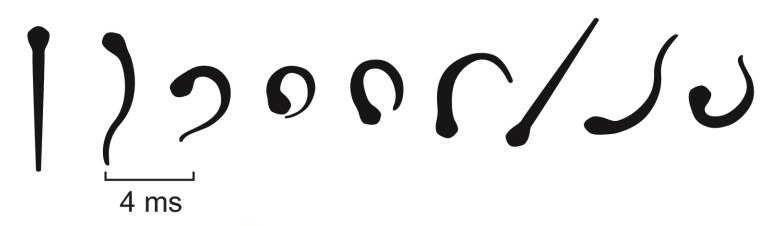
\includegraphics[width=8cm,height=3cm]{ZEBRAFISH_C_ESCAPE.jpg}
\caption{Digital example of a zebrafish startle/escape locomotor pattern. Graphics taken from article \textit{Auditory sensitivity of larval zebrafish (Danio rerio) measured using a behavioral prepulse inhibition assay} by Bhandiwad A. A. \textit{et al.}, published at \textcopyright 2013 The Company of Biologists Ltd\cite{ref21}. }
\end{center}
\end{figure}
\\
Locomotor patterns have been generally researched as action sequences\cite{ref22} in association with diseases like schizophrenia\cite{ref23} and Parkinson’s disease\cite{ref24}, where it has been shown that abnormal execution or the disability to perform several movements in a sequence can be seen as disease symptoms, which would otherwise not be detected when observing single movements only.\\
Drug screening processes, based on an experimental setup involving longitudinal measurements of zebrafish locomotor patterns in several different conditions, require careful data preprocessing and analysis\cite{ref25}\cite{ref26}. Mixed effects, multicollinearity, high variation in within and between subject variance, data distribution, zero inflation and many other aspects of the analysis have to be considered. Adequate large scale data handling and analysis are becoming the bottleneck of high-throughput screening processes. Robust and fully automated preprocessing and analysis pipelines are required to efficiently obtain accurate results needed for drug screening.
\\In this project, several zebrafish locomotor data preprocessing and analysis pipelines were designed, implemented and tested, including data filtering, extraction of descriptive statistics of locomotor phenotypes, comparative exploratory data analysis and mixed effects analysis.
\section{Methods}
\subsection{Experimental design}
Movement of zebrafish larvae, 10 days post fertilisation, was recorded in constant dark. Animal ethics, fish maintenance, video recording and movement tracking described in detail in published studies\cite{ref17}\cite{ref18}. \\Zebrafish larvae were recorded in four different conditions, normal condition, serving as a healthy model and three neurological disease induced conditions, serving as a sedated/hypoactive model and two types of a stressed/hyperactive model, details in Apendix A.1. Sedated/hypoactive state was induced by an administration of a low dose of Apomorphine(0.5 $\mu$M), first type of a stressed/hyperactive state was induced by an administration of a high dose of Apomorphine(50 $\mu$M) and the second type of a stressed/hyperactive state was induced by administration of PTZ(2.5 mM). Eleven different compounds were screened in all four conditions, Aripiprazole\cite{ref27}, Cariprazine\cite{ref28}, Clozapine\cite{ref29}, Clozapine N-oxide (CNO)\cite{ref30}, Haloperidol\cite{ref31}, N-desmethylclozapine(NDMC)\cite{ref32}, OSU6162\cite{ref33}, PCAP1\cite{ref34}, PCAP2\cite{ref34} and two novel compounds PCAP3 and PCAP4. All eleven compounds were evaluated in three different doses, 1 $\mu$M, 3 $\mu$M and 10 $\mu$M  with an additional control group. NDMC was also evaluated at 25 $\mu$M, 50 $\mu$M and 100 $\mu$M with an additional control group and was therefore considered as an extra compound named NDMCHigh. This resulted in four sets of twelve assays per each of the four conditions.
Each assay was conducted on 12 zebrafish larvae, recorded for 65 minutes with a 1 minute pause every 5 minutes, schematic and tabular illustrations of the experimental setup in Figure 3.
\begin{figure}[h]
\begin{center}
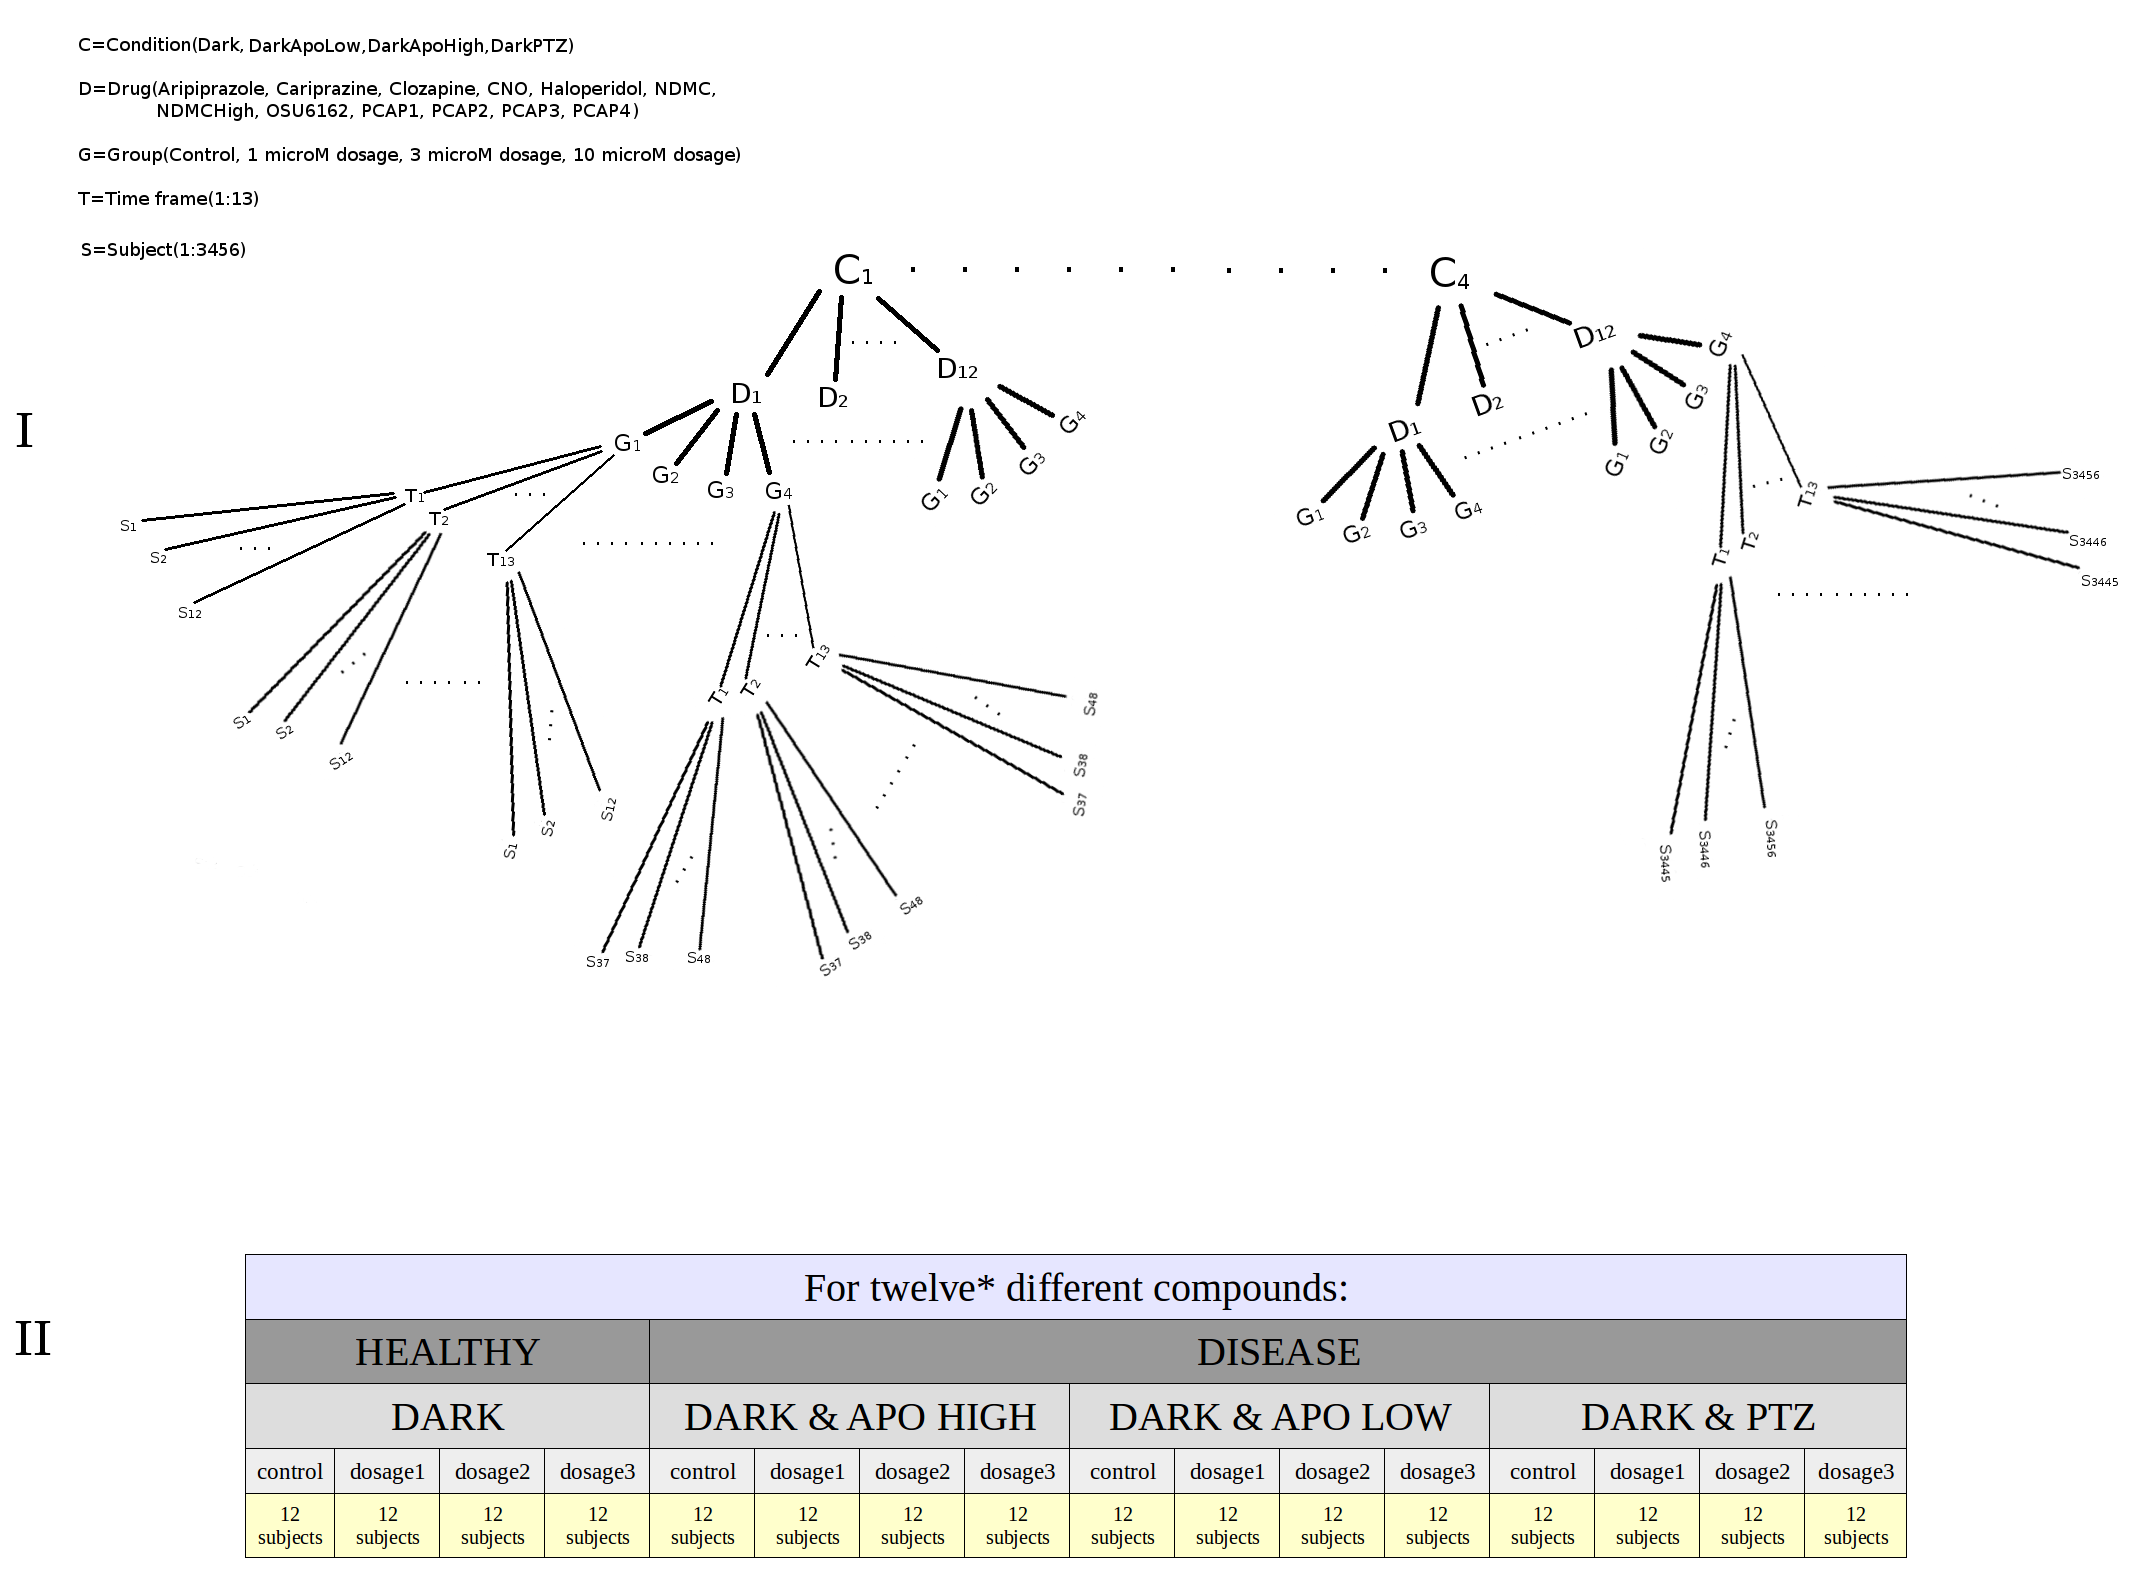
\includegraphics[width=17cm,height=12.5cm]{expdesignComb.png}
\caption{(\textbf{I})Schematic illustration of the experimental setup, showing the nested and crossed components. (\textbf{II}) Tabular illustration of the experimental setup. *NDMC in high doses is counted as an extra compound.}
\end{center}
\end{figure}
\\\\
Data resulting from assays, where none of the eleven compounds was administrated, was merged together into measurements of 144 zebrafish larvae, to serve as a control reference for each of the four conditions. The control reference of the healthy condition was taken as the general control reference for the entire experimental setup. 
\subsection{Data analysis}
\subsubsection{Data format}
Zebrafish larval movement was recorded and tracked, producing an action sequence per subject, per time frame, per assay. \\Prior to data analysis, zebrafish larval movement was preprocessed and classified into 8 different turn types, organized in swim bouts, classification described in detail in published studies\cite{ref18}. All together, eleven codons were used. \\Eight codons for eight different turn types(turn type differentiation explained in Appendix A.2), a codon separating bouts and two codons indicating left or right direction:
\begin{itemize}
\item \textbf{s}, turn codon for \textbf{Scoots}, representing normal/exploration behaviour, the most common movement of the zebrafish larvae,
\item \textbf{c}, turn codon for \textbf{C-bends}, representing startle/escape behaviour,
\item \textbf{o}, turn codon for \textbf{O-bends}, representing startle/escape behaviour, 
\item \textbf{j}, turn codon for \textbf{J-bends}, representing predatory behaviour,
\item \textbf{e}, turn codon for \textbf{E-bends}, unidentified turn type, currently termed as a routine turn,
\item \textbf{g}, turn codon for \textbf{G-bends}, unidentified turn type, currently termed as a routine turn, 
\item \textbf{h}, turn codon for \textbf{H-bends}, unidentified turn type, currently termed as a routine turn, 
\item \textbf{i}, turn codon for \textbf{I-bends}, unidentified turn type, currently termed as a routine turn,  
\item \textbf{b}, bout codon separating between the bouts,  
\item \textbf{r}, direction codon, indicating right direction,  
\item \textbf{l}, direction codon, indicating left direction. 
\end{itemize}
Resulting action sequence was then stored in a fasta format file per compound, per condition. Information regarding the condition, subject, compound, dosage, absolute and relative time was coded in the information line, example in Figure 4.
\begin{figure}[h!]
\begin{center}
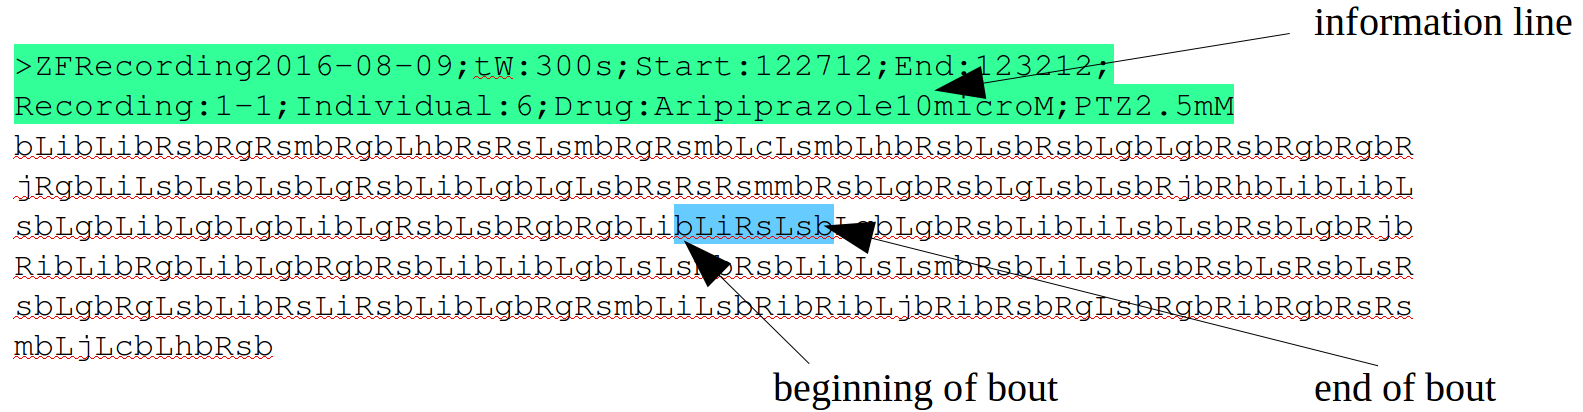
\includegraphics[width=16cm,height=4cm]{action_seq_ex.png}
\caption{Example of an action sequence, recorded on the 9th of August, 2016, lasting for 300s, starting at relative position 122712, ending at relative position 123212, being the first recording out of thirteen, for the sixth subject out of twelve, with an administration of 10 $\mu$M of Aripiprazole along with 2.5 mM of PTZ.}
\end{center}
\end{figure}
\newpage
\subsubsection{Descriptive statistics}
Descriptive statistics were derived from the action sequences to serve as zebrafish larvae locomotor phenotypes. Some of the statistics were additionaly derived per stratum of another statistics, due to multicollinearity. For each action sequence, the following descriptive statistics were derived:
\begin{itemize}
\item Action sequence length,
\item Total bout frequency per action sequence(bout count),
\item Frequency of bouts of length N(length N bout count),
\item Proportion of length N bouts in total bout count(length N bout count proportion),
\item Proportions of the eight different turns(Scoots, C-bends, O-bends, J-bends, E-bends, G-bends, H-bends, I-bends proportion), 
\item Proportions of the eight different turns, per bout length N(length N Scoots, C-bends, O-bends, J-bends, E-bends, G-bends, H-bends, I-bends proportion),
\item Proportions of length two transitions, out of all words of length two, for all 64 possible transitions(transition TT proportion),
\item Proportions of length two transitions, out of all words of length two, for all 64 possible transitions, per bout length N(length N transition TT proportion),  
\item Proportions of length three transitions, out of all words of length three, for all 512 possible transitions(transition TTT proportion),
\item Proportions of length three transitions, out of all words of length three, for all 512 possible transitions, per bout length N(length N transition TTT proportion), 
\end{itemize}
where $N\in [1,2,3,4,5,6+]$ and $T\in [s,c,o,j,e,g,h,i]$.
\\To simplify the exploratory data analysis and the mixed effects analysis, all the descriptive statistics were averaged over all subjects per time frame in each of the assays, resulting in the following dataframe structure:\\
\tiny{timeframe {\hspace{1cm}} asssay {\hspace{1cm}} variable1 {\hspace{1cm}} variable2 {\hspace{1cm}} .... {\hspace{1cm}} variableN}
\\ \-\ \hspace{0.5cm}1\hspace{1.4cm}"assay 1"\hspace{1.5cm}x\hspace{2cm}x\hspace{1.64cm}....\hspace{1.6cm}x
\\ \-\ \hspace{0.5cm}2\hspace{1.4cm}"assay 1"\hspace{1.5cm}x\hspace{2cm}x\hspace{1.64cm}....\hspace{1.6cm}x
\\ \-\ \hspace{0.5cm}.\hspace{1.47cm}"assay 1"\hspace{1.5cm}x\hspace{2cm}x\hspace{1.64cm}....\hspace{1.6cm}x
\\ \-\ \hspace{0.5cm}.\hspace{1.47cm}"assay 1"\hspace{1.5cm}x\hspace{2cm}x\hspace{1.64cm}....\hspace{1.6cm}x
\\ \-\ \hspace{0.5cm}.\hspace{1.47cm}"assay 1"\hspace{1.5cm}x\hspace{2cm}x\hspace{1.64cm}....\hspace{1.6cm}x
\\ \-\ \hspace{0.5cm}13\hspace{1.3cm}"assay 1"\hspace{1.5cm}x\hspace{2cm}x\hspace{1.64cm}....\hspace{1.6cm}x
\\ \-\ \hspace{0.5cm}1\hspace{1.4cm}"assay 2"\hspace{1.5cm}x\hspace{2cm}x\hspace{1.64cm}....\hspace{1.6cm}x
\\ \-\ \hspace{0.5cm}2\hspace{1.4cm}"assay 2"\hspace{1.5cm}x\hspace{2cm}x\hspace{1.64cm}....\hspace{1.6cm}x
\\ \-\ \hspace{0.5cm}.\hspace{1.85cm}.\hspace{2.1cm}x\hspace{2cm}x\hspace{1.64cm}....\hspace{1.6cm}x
\\ \-\ \hspace{0.5cm}.\hspace{1.85cm}.\hspace{2.1cm}x\hspace{2cm}x\hspace{1.64cm}....\hspace{1.6cm}x
\\ \-\ \hspace{0.5cm}.\hspace{1.85cm}.\hspace{2.1cm}x\hspace{2cm}x\hspace{1.64cm}....\hspace{1.6cm}x
\\ \-\ \hspace{0.5cm}13\hspace{1.3cm}"assay M"\hspace{1.38cm}x\hspace{2cm}x\hspace{1.64cm}....\hspace{1.6cm}x
\\ \-\ \hspace{0.5cm}\hspace{1.3cm}\hspace{1.38cm}\hspace{2cm}\hspace{1.64cm}\hspace{1.6cm}
\\ \-\ \hspace{0.5cm}\hspace{1.3cm}\hspace{1.38cm}\hspace{2cm}\hspace{1.64cm}\hspace{1.6cm}
\normalsize
\\To explore multicollinearity, Spearman's rank correlation was tested between certain descriptive statistics.
\subsubsection{Outliers}
Technical outliers can occur due to malfunctions of the tracking software. \\The tracking software was designed to constantly track the zebrafish larva. If the larva is still for a time period longer then five minutes, the tracking software can encounter difficulties locating it and will, therefore, move around the well, producing an erroneous action sequence. Several such cases were detected manually in two assays, resulting in a small set of known outliers.
Using machine learning methods, the set of known outliers was modelled, to enable an automatic detection of outliers in the rest of the assays.
Ten descriptive statistics per subject over time frames were chosen and used as features in the machine learning process:
\begin{itemize}
\item Bout frequency per action sequence.
\item Length of the action sequence.
\item Proportions of each of the eight different turns. 
\end{itemize}
Dataset, to be used in the machine learning process, consisted of positive and negative outliers of the two assays which were observed manually. The class of negative outliers was substantially oversized, with the ratio 99:1. To ensure an unbiased learning process, the oversized class needed to be undersampled and the undersized class oversampled. \\Undersampling was achieved by randomly removing approximately a third of the negative outliers. Oversampling was achieved with the oversampling method SMOTE\cite{ref35}, synthesising approximately 390 positive outliers. The ratio between the positive and negative class of the resulting dataset was 33:67 respectively. The resampled dataset was halved into a learning and a test set.
Modelling was performed with a \textit{Random forest} algorithm\cite{ref36}, using 2000 trees.

\subsubsection{Exploratory data analysis}
Exploratory data analysis was conducted with a Principal component analysis(PCA)\cite{ref37} over a set of descriptive statistics. \\In PCA, the input data set is mapped into a new coordinate system, using an orthogonal linear transformation. The resulting variables are linearly uncorrelated and are called principal components. The formulation of the transformation ensures that the explained variance by each of the principal components will decrease linearly by their order, while each of the principal components is orthogonal to the preceding components. Consequentially, only the first few principal components can sufficiently represent the variation of the entire set, resulting in a large reduction in dimensionality and therefore easier visualisation.\\R-package \textit{FactoMineR}\cite{ref38}, with the function \textit{PCA}, was used as a readily available implementation of PCA. \\To explore the compound effects on the healthy and disease induced larvae, in different dosages and in different conditions, the first two principal components were visualised, for each of the three disease induced conditions combined with the healthy condition. Since the number of variables differed for each condition, the intersection with the healthy condition data set was taken for each. PCA results were additionally summarized and plotted with respect to the direction of change in time or of change in dosage. With respect to the direction of change in time, a vector was drawn from the first to the last timeframe, for all compounds and plotted together with the healthy control and the disease induced control, for each of the three different dosages. With respect to the change in dosage, an average was taken over all thirteen timeframes and a curved vector was drawn over all three averages of the three different dosages, for all compounds and plotted together with the two controls, also averaged in time. For the purpose of ranking the descriptive statistics according to their influence, the sum of squared correlation coefficients with the first five principal components was explored. For the purpose of ranking the compounds and their dosages, in their effect on the healthy and disease induced larvae, Euclidean distance was calculated between the first five principal components of the different experimental groups. Euclidean distances between the principal components were also used to construct a distance tree, in order to visualise similarity between the compounds in their effect on the healthy and disease induced larvae. Trees were saved in a Newick format and uploaded to Evolview\cite{ref39}, to design a better visualisation.
\\Results were obtained for several sets of descriptive statistics, including total bout count, bout count proportions per bout length, turn and turn transition proportions. The sets of descriptive statistics differed in whether the descriptive statistics of turns and turn transitions were stratified in bout length and whether descriptive statistics of bout counts were included. 
\subsubsection{Mixed effects analysis}
Mixed effects analysis was performed in order to obtain compound effect sizes in different conditions and dosages, through several time frames, with a reference to the healthy control, while adjusting for covariates. Due to variable distributions, high variance through the time frames and multicollinearity, a generalized linear model(GLM) was constructed. A readily available implementation of GLM, R-function \textit{glm} was used, based on a Quasipoisson distribution, due to a significant difference of mean and variance. \\All descriptive statistics were modelled with a variable representing the experimental groups, a variable representing time frames and their multiplicative term. Model of descriptive statistics, derived from bout count, was not adjusted for any other descriptive statistics. Model of descriptive statistics, derived from turn proportions, was adjusted for descriptive statistics derived from bout count. Model of descriptive statistics, derived from turn transition proportions, was adjusted for descriptive statistics derived from bout count and turn proportions. 
\\The largest effects obtained from the analysis were presented in a heatmap, colour coded according to the size of the effect with an additional notation representing the significance level. Heatmaps were constructed and plotted with the R function \textit{heatmap.2} from the package \textit{gplot}\cite{ref40}. Besides the typical colour coding of the values, the function \textit{heatmap.2} additionally reorders the rows and columns by constructing an Euclidean distance based dendrogram and therefore providing variable and compound ranking within the heatmap.
\section{Results}
\subsection{Descriptive statistics}
Descriptive statistics are meant to represent locomotor phenotypes and summarize the information that would separate between the assays or between the positive or negative outliers. Descriptive statistics were obtained from the action sequences, where bout was the operational unit. The number of descriptive statistics was not the same through the four different conditions, since some of the very rare transitions only occured in some conditions. Total number of descriptive statistics per condition in Table 1.
\begin{table}[h!]
  \begin{center}\tiny
    \begin{tabular}{|c|c|c|c|c|c|c|c|c|}
    \hline
     &\multicolumn{2}{c|}{\begin{tabular}[c]{@{}c@{}c@{}}healthy\\condition\\\end{tabular}}&\multicolumn{2}{c|}{\begin{tabular}[c]{@{}c@{}c@{}}hypoactive\\condition\\\end{tabular}}&\multicolumn{2}{c|}{\begin{tabular}[c]{@{}c@{}c@{}}hyperactive\\condition I\\\end{tabular}}&\multicolumn{2}{c|}{\begin{tabular}[c]{@{}c@{}c@{}}hyperactive\\condition II\\\end{tabular}}\\ \cline{2-9}
       &\begin{tabular}[c]{@{}c@{}c@{}}not stratified\\in bout length\end{tabular}&\begin{tabular}[c]{@{}c@{}c@{}}stratified in\\bout length\end{tabular} & \begin{tabular}[c]{@{}c@{}c@{}}not stratified\\in bout length\end{tabular}&\begin{tabular}[c]{@{}c@{}c@{}}stratified in\\bout length\end{tabular}&\begin{tabular}[c]{@{}c@{}c@{}}not stratified\\in bout length\end{tabular}&\begin{tabular}[c]{@{}c@{}c@{}}stratified in\\bout length\end{tabular}&\begin{tabular}[c]{@{}c@{}c@{}}not stratified\\in bout length\end{tabular}&\begin{tabular}[c]{@{}c@{}c@{}}stratified in\\bout length\end{tabular} \\ \hline 
       \begin{tabular}[c]{@{}c@{}c@{}}Total of\\descriptive\\statistics\end{tabular}&375&1094&290&818&541&1796&580&2156 \\ \hline
    \end{tabular}
  \end{center}
    \caption{Number of extracted descriptive statistics in each of the four conditions.}
\end{table}
\\Total bout count per bout length visually differed between the controls of the different conditions, an example in Appendix B.1.1, where it is clear, that bouts of length 6 and more, are relatively rare, compared to the majority of length one and two bouts, especially in the healthy and the hypoactive condition. \\When examining the total bout count per length through the 13 time frames, changes were visible and reflected the larva's habituation and response to the environment, an example in Appendix B.1.2, showing changes through the time frames for each condition.
\\Examples in Appendix B.2.1 show a strong visual correlation between the turn proportions and bout length, indicating an issue of multicollinearity. Table 2 shows the results of a Spearman's rank correlation test, when comparing bout length to each of the eight different turn type proportions in a dataset consisting of all available data.
\begin{table}[h!]\tiny
\centering

\begin{tabular}{|c|c|c|}
\hline
\begin{tabular}[c]{@{}c@{}c@{}} \\\hfill \\\hfill \end{tabular}                  & Spearman's ro & p-value        \\ \hline
\begin{tabular}[c]{@{}c@{}c@{}} \\Scoots Proportion \\\hfill \end{tabular} & 0.29          & \textless2e-16 \\ \hline
\begin{tabular}[c]{@{}c@{}c@{}} \\C-Bends Proportion \\\hfill \end{tabular} & 0.02          & \textless2e-16 \\ \hline
\begin{tabular}[c]{@{}c@{}c@{}} \\O-Bends Proportion \\\hfill \end{tabular} & 0.04          & \textless2e-16 \\ \hline
\begin{tabular}[c]{@{}c@{}c@{}} \\J-Bends Proportion \\\hfill \end{tabular} & -0.01         & \textless2e-16 \\ \hline
\begin{tabular}[c]{@{}c@{}c@{}} \\G-Bends Proportion \\\hfill \end{tabular} & -0.03         & \textless2e-16 \\ \hline
\begin{tabular}[c]{@{}c@{}c@{}} \\H-Bends Proportion \\\hfill \end{tabular} & 0.01          & \textless2e-16 \\ \hline
\begin{tabular}[c]{@{}c@{}c@{}} \\E-Bends Proportion \\\hfill \end{tabular} & -0.03         & \textless2e-16 \\ \hline
\begin{tabular}[c]{@{}c@{}c@{}} \\ I-Bends Proportion\\\hfill \end{tabular} & -0.01         & \textless2e-16 \\ \hline
\end{tabular}
\caption{Spearman's correlation coefficients when comparing bout length to the proportions of each of the eight different turn types.}
\end{table}
\\To avoid confounding, stratification in bout length was performed, where bouts of length six turns and more were joined as one stratum, due to the low count of longer bouts.
While this will avoid confounding with bout length, the total bout count per length might still influence the proportion of turns. Examples of compound effects for Haloperidol, Clozapine and NDMC in Appendix B.2.2, where different effects on the healthy and disease induced larvae can be seen through time, with some cases showing a similar trend in turn proportions and bout count per bout length.
\\Transition proportions will also be subjected to confounding by bout length, bout count and even further by turn proportions, since an increase in for example transition "sg" might be only due to an increase in Scoots and G-bends. Partial Spearman's rank correlation coefficient was significant at 0.19, when testing partial correlation between the proportion of "sg" transitions and proportion of G-Bends, adjusted for bout count and bout length descriptive statistics. \\Visual observations of transition frequencies also show a high count of transitions including routine or normal behaviour turns, an example in Appendix B.3.1, while the transitions including startle/escape turns are rare and might be insufficient to detect a significant trend. To test the significance of the trends visually observed in the descriptive statistics and further adjust for confounding factors, appropriate statistical analyses were performed.
\subsection{Outliers detection and removal}
Outliers were detected automatically with a model of a set of manually detected outliers.
The values of the descriptive statistics, used as features, separated well between the positive and negative outliers, an example in Figure 6.1.
Upon testing the \textit{Random forest} model of outliers, the classification accuracy was 0.995, sensitivity was 0.993, specificity 100 and precision 100. Classification also appeared successful in a visual observation, an example in Figure 6.2. Alltogether, approximately 1.34 \% of action sequences were detected as outliers and were therefore removed.
\begin{figure}[h!]
\begin{center}
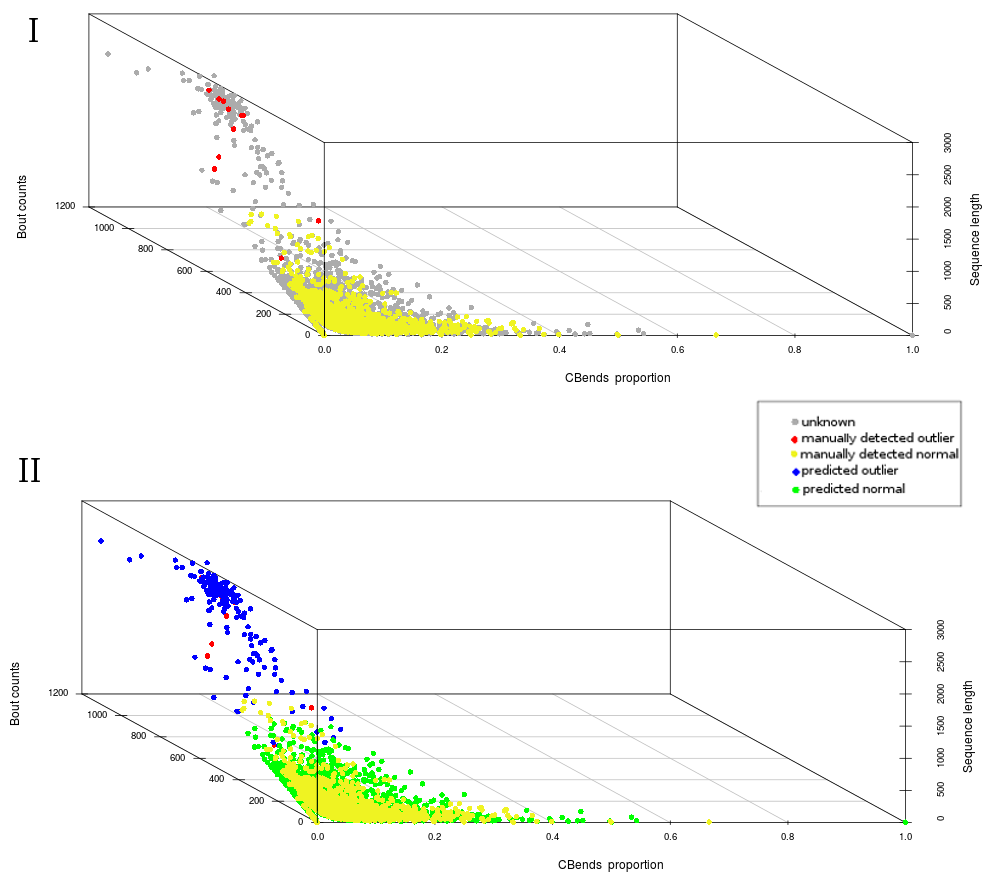
\includegraphics[width=10cm,height=10cm]{outliersEx.png}
\caption{Classification of all action sequences in the hypoactive condition.(\textbf{I})Action sequence length, bout count and C-bends proportion in a 3D plot of manually detected positive(red), negative(yellow) and unknown(grey) outliers.(\textbf{II})Action sequence length, bout count and C-bends proportion in a 3D plot of manually detected positive(red), manually detected negative(yellow), predicted positive(blue) and predicted negative(green) outliers.}
\end{center}
\end{figure}
\newpage
\subsection{Exploratory data analysis}
PCA was conducted on four sets of descriptive statistics:
\begin{itemize}
\item A set containing all descriptive statistics, including bout count, turn and turn transition proportion statistics, where turn and turn transition proportions were not stratified in bout length.
\item A set containing only the turn and turn transition proportion statistics, where turn and turn transition proportions were not stratified in bout length.
\item A set containing all descriptive statistics, including bout count, turn and turn transition proportion statistics, where turn and turn transition proportions were stratified in bout length. 
\item A set containing only the turn and turn transition proportion statistics, where turn and turn transition proportions were stratified in bout length.
\end{itemize}
First and second principal components were visualised for all four sets by colour coding according to the different conditions, dosages and time progress. \\An example for one of the compounds in the hypoactive, type I hyperactive and type II hyperactive condition, using the first set of descriptive statistics is shown in Figures 6.1, 6.2 and 6.3, respectively, where compound effects can be seen in the aspects of the proximity to the healthy or disease induced control cluster. Plots for all 12 compounds, for all three conditions and all four sets of descriptive statistics are shown in the Appendix C.1.
\newpage
\begin{figure}[h!]
\begin{center}
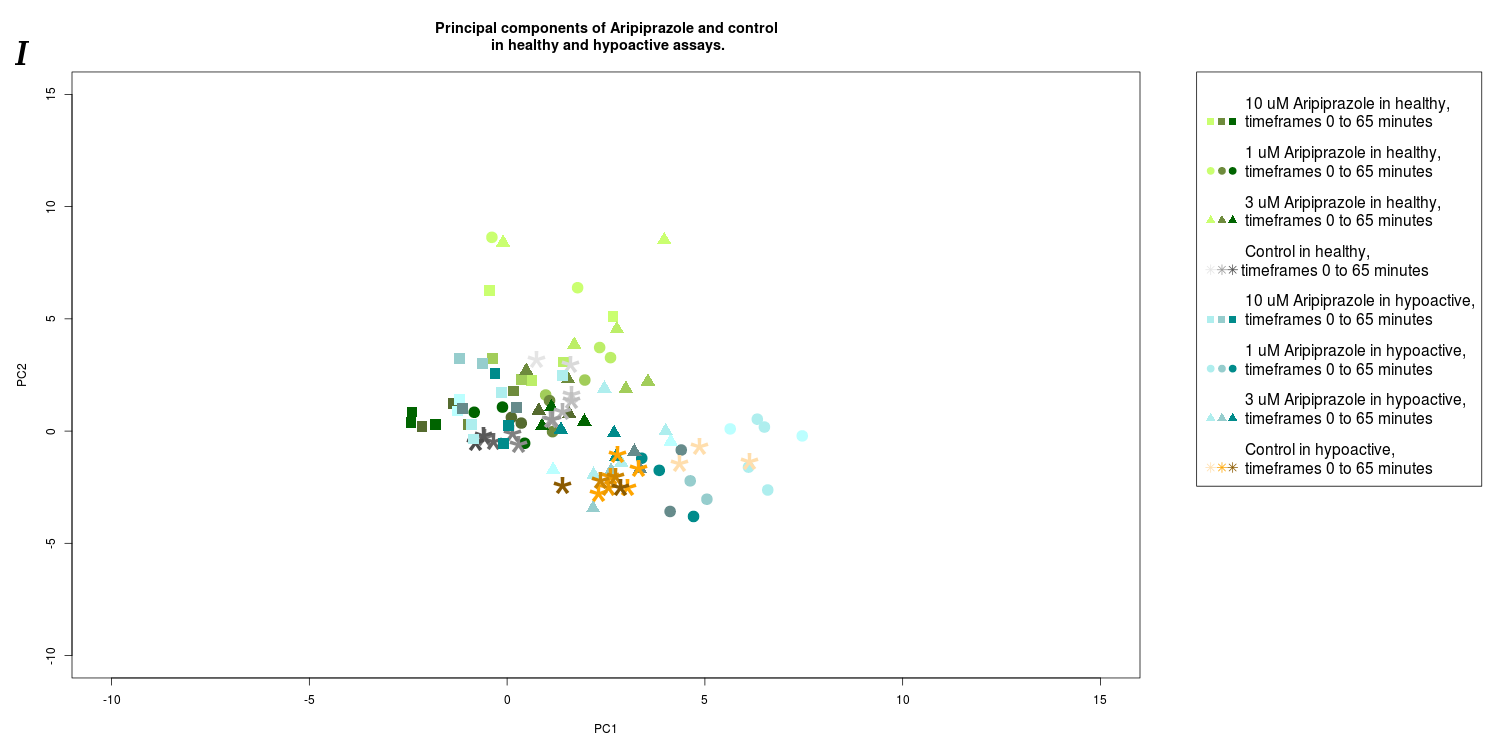
\includegraphics[width=16cm,height=8cm]{Aripiprazole_Control_DarkApoLow.png}
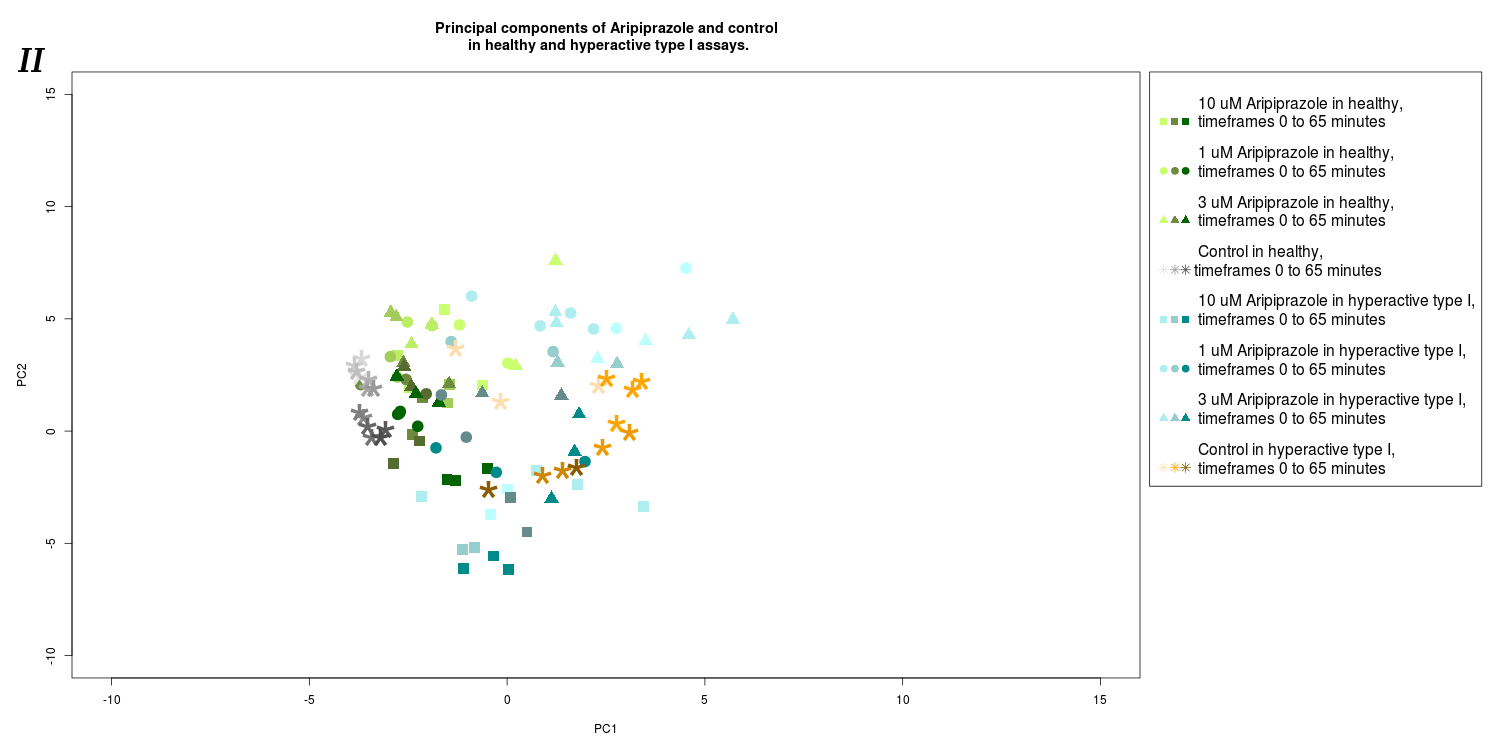
\includegraphics[width=16cm,height=8cm]{Aripiprazole_Control_DarkApoHigh.png}
\end{center}
\end{figure}
\newpage
\begin{figure}[h!]
\begin{center}
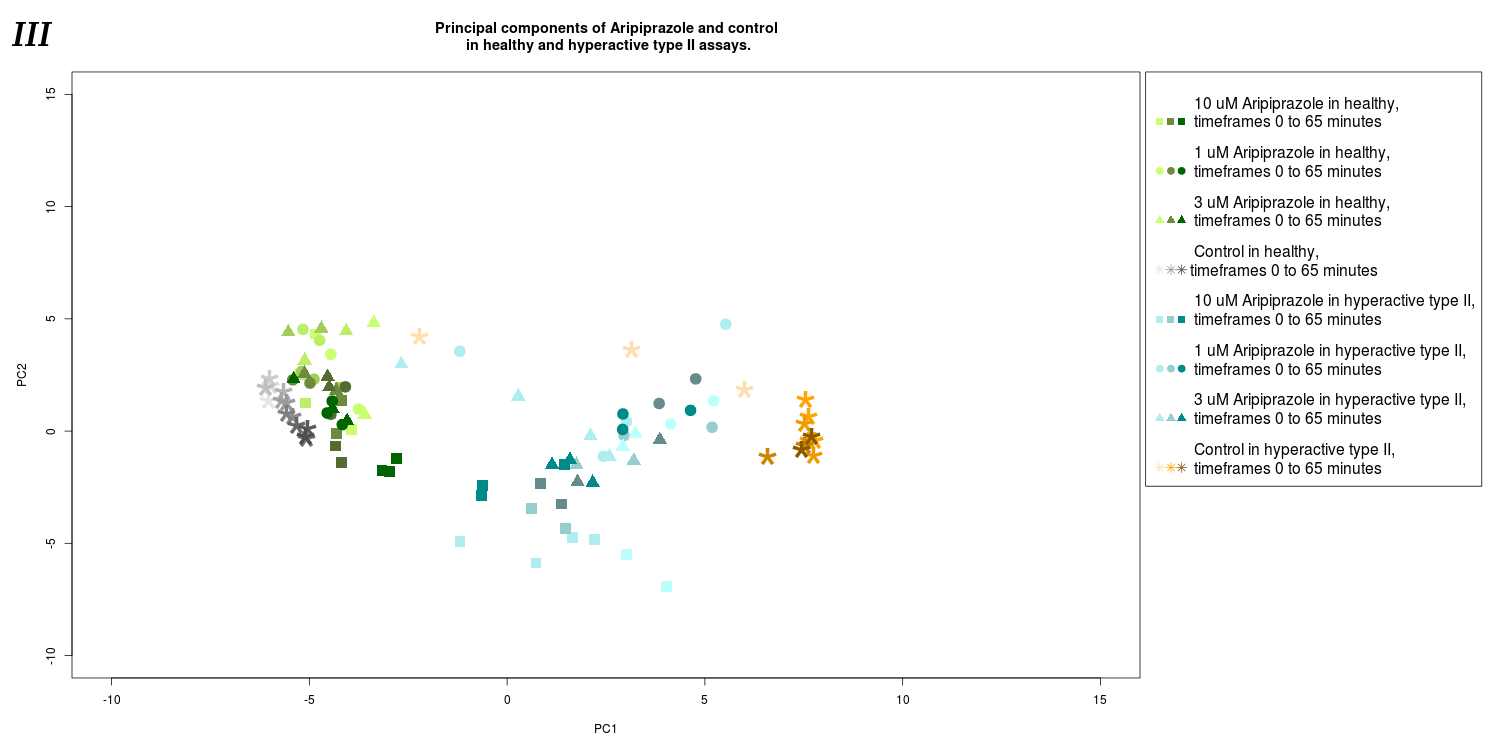
\includegraphics[width=16cm,height=8cm]{Aripiprazole_Control_DarkPTZ.png}
\caption{By using the first set of descriptive statistics, the first and second PC of the control in healthy(grey star) and the control in the (\textbf{I})hypoactive, (\textbf{II}) type I hyperactive and (\textbf{III})type II hyperactive control(orange star) along with Aripiprazole in three different dosages(square for a high dose, triangle for a medium dose and a circle for a low dose) in the healthy condition(green) and in the disease induced condition(blue). Colour intensity coded by progress in time.}
\end{center}
\end{figure}
\\Although the four different clusters(the control in the healthy condition, the compound in the healthy condition, the control in the disease induced condition and the compound in the disease induced condition) separated relatively well, the amount of cumulative accounted variance by the first five principal components was low, ranging from approximately 12\% to 21\%. Low accounted variance was due to the large amount of extremely rare transitions, which did not contain enough information, but still influenced the amount of accounted variance by the first principal component. When reducing the number of variables to the first 50 most influential descriptive statistics, the cumulative variation, accounted by the first five principal components, increased to approximately 75\% to 88\%.
\\Variable influence was determined based on the sum of squared correlation coefficients when comparing to the first five principal components. Table 3 shows the first 10 most influential descriptive statistics for each of the three disease induced conditions, on a set of all descriptive statistics, where turn and transition proportions were not stratified in bout length. A longer list of descriptive statistics ranked according to their influence for all three conditions and all four sets of descriptive statistics is shown in Appendix C.2. 
% Please add the following required packages to your document preamble:
% \usepackage{multirow}
\begin{table}[h!]\tiny
\centering
\begin{tabular}{|c|c|c|c|}
\hline
                                                    & \begin{tabular}[c]{@{}c@{}}hypoactive\\condition\end{tabular}                &\begin{tabular}[c]{@{}c@{}} type I hyperactive\\condition \end{tabular}              & \begin{tabular}[c]{@{}c@{}}type II hyperactive\\condition\end{tabular}                \\ \hline
\begin{tabular}[c]{@{}c@{}c@{}c@{}c@{}}First 10\\most influential\\descriptive\\statistics\\\end{tabular} & C-Bends Proportion                  & E-Bends Proportion                  & E-Bends Proportion                  \\ \cline{2-4} 
\begin{tabular}[c]{@{}c@{}c@{}c@{}} \\ \\ \\\end{tabular}                                                    & Scoots Proportion                   & Transition ii Proportion            & Length 4 Bout Count Proportion      \\ \cline{2-4} 
\begin{tabular}[c]{@{}c@{}c@{}c@{}} \\ \\ \\\end{tabular}                                                     & Transition sss Proportion           & Transition gg Proportion            & Length 1 Bout Count Proportion      \\ \cline{2-4} 
\begin{tabular}[c]{@{}c@{}c@{}c@{}} \\ \\ \\\end{tabular}                                                     & Transition ss Proportion            & Transition ssg Proportion           & Length 6 Plus Bout Count Proportion \\ \cline{2-4} 
\begin{tabular}[c]{@{}c@{}c@{}c@{}} \\ \\ \\\end{tabular}                                                     & I-bends Proportion                   & Transition ee Proportion            & Transition se Proportion            \\ \cline{2-4} 
 \begin{tabular}[c]{@{}c@{}c@{}c@{}} \\ \\ \\\end{tabular}                                                    & H-bends Proportion                   & Length 4 Bout Count Proportion      & Transition ee Proportion            \\ \cline{2-4} 
\begin{tabular}[c]{@{}c@{}c@{}c@{}} \\ \\ \\\end{tabular}                                                     & Transition cs Proportion            & Transition es Proportion            & Transition es Proportion            \\ \cline{2-4} 
\begin{tabular}[c]{@{}c@{}c@{}c@{}} \\ \\ \\\end{tabular}                                                     & Transition css Proportion           & Transition sgg Proportion           & Transition sse Proportion           \\ \cline{2-4} 
\begin{tabular}[c]{@{}c@{}c@{}c@{}} \\ \\ \\\end{tabular}                                                     & Transition is Proportion            & Length 6 Plus Bout Count Proportion & Length 2 Bout Count Proportion      \\ \cline{2-4} 
\begin{tabular}[c]{@{}c@{}c@{}c@{}} \\ \\ \\\end{tabular}                                                     & J-bends Proportion                   & Transition se Proportion            & Transition see Proportion           \\ \cline{2-4} 
\begin{tabular}[c]{@{}c@{}c@{}c@{}} \\ \\ \\\end{tabular}                                                     & Length 5 Bout Count Proportion      & Transition ggg Proportion           & Length 5 Bout Count Proportion       \\ \hline
\end{tabular}
\caption{By using the first set of descriptive statistics, the first 10 most correlated descriptive statistics in each of the three disease induced conditions, when compared to the first five principal components.}
\end{table}
\newpage
The first ten most influential variables will also include descriptive statistics derived from bout count and bout length. Bout count and bout length have already been analysed in published studies\cite{ref18}\cite{ref19} and are therefore of lesser interest than descriptive statistics derived from turns and turn transitions. Even though multicollinearity is not problematic for PCA, the high correlation between the bout count, bout length and turn proportions was still an issue, since the variance of turns and turn transitions could not be explored separately. When conducting PCA on the second set of descriptive statistics, using turn and turn transition proportion descriptive statistics only, most of the results were very similar as above, with the exception of the hypoactive condition, examples shown in Figures 7.1, 7.2 and 7.3, respectively. First 10 most influential descriptive statistics for each of the three disease induced conditions, using the second set of descriptive statistics, are shown in Table 4. 
Cumulative variance accounted by the first five principal components ranged from approximately 10\% to 19\% with the entire second set of descriptive statistics, while for the set of the first 50 most influential descriptive statistics, the first principal components accounted for approximately 69\% to 84\% of total variance.\\
\newpage
\begin{figure}[h!]
\begin{center}
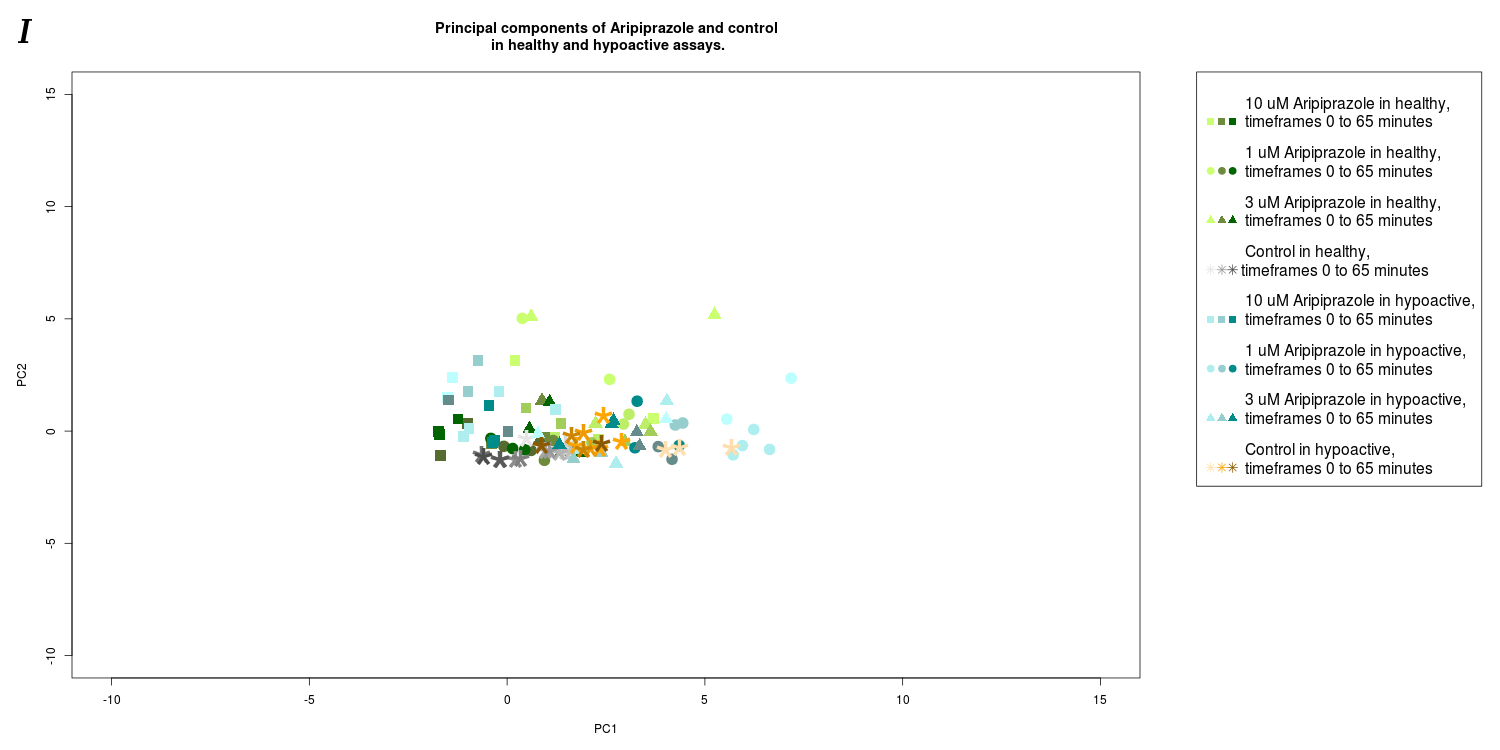
\includegraphics[width=16cm,height=8cm]{Aripiprazole_Control_DarkApoLow_turn_only.png}
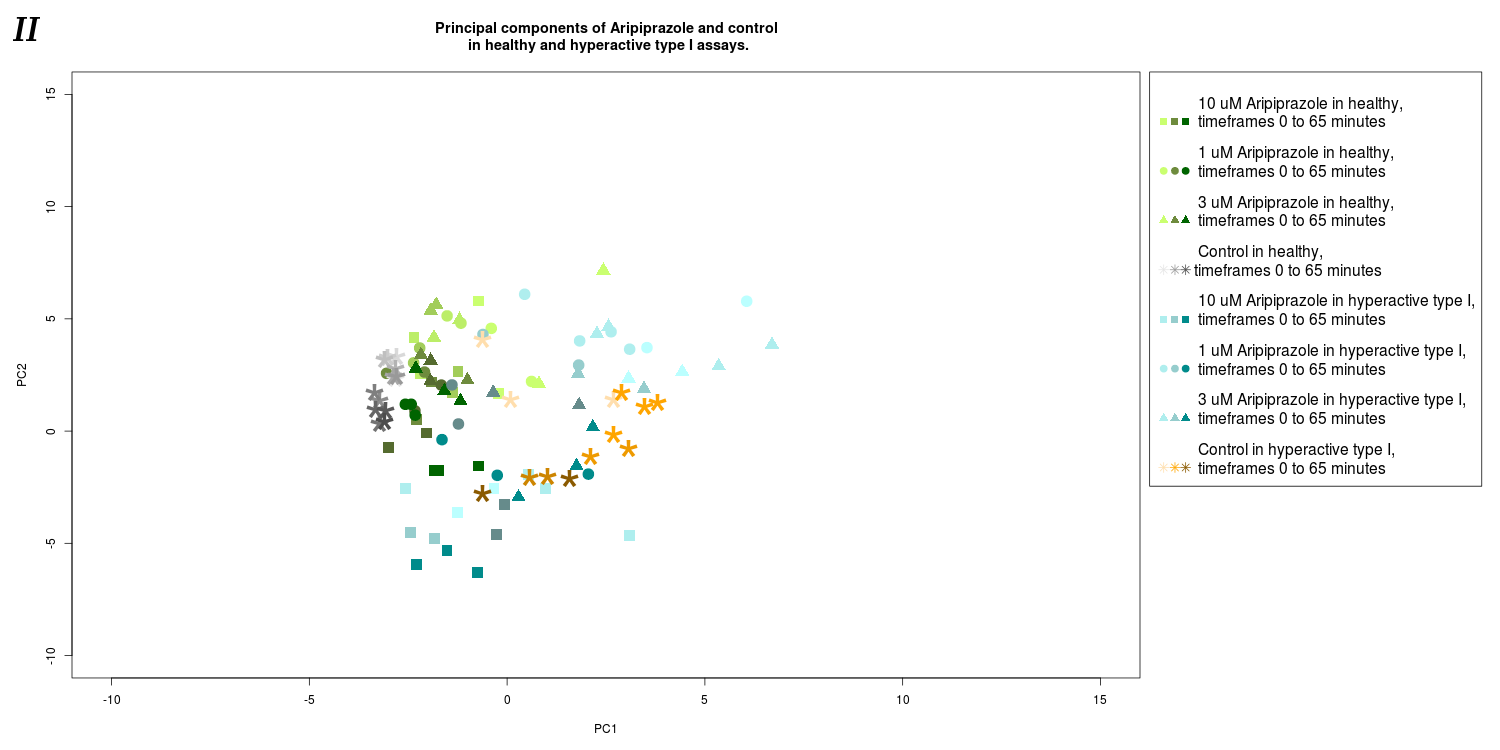
\includegraphics[width=16cm,height=8cm]{Aripiprazole_Control_DarkApoHigh_turn_only.png}
\end{center}
\end{figure}
\newpage
\begin{figure}[h!]
\begin{center}
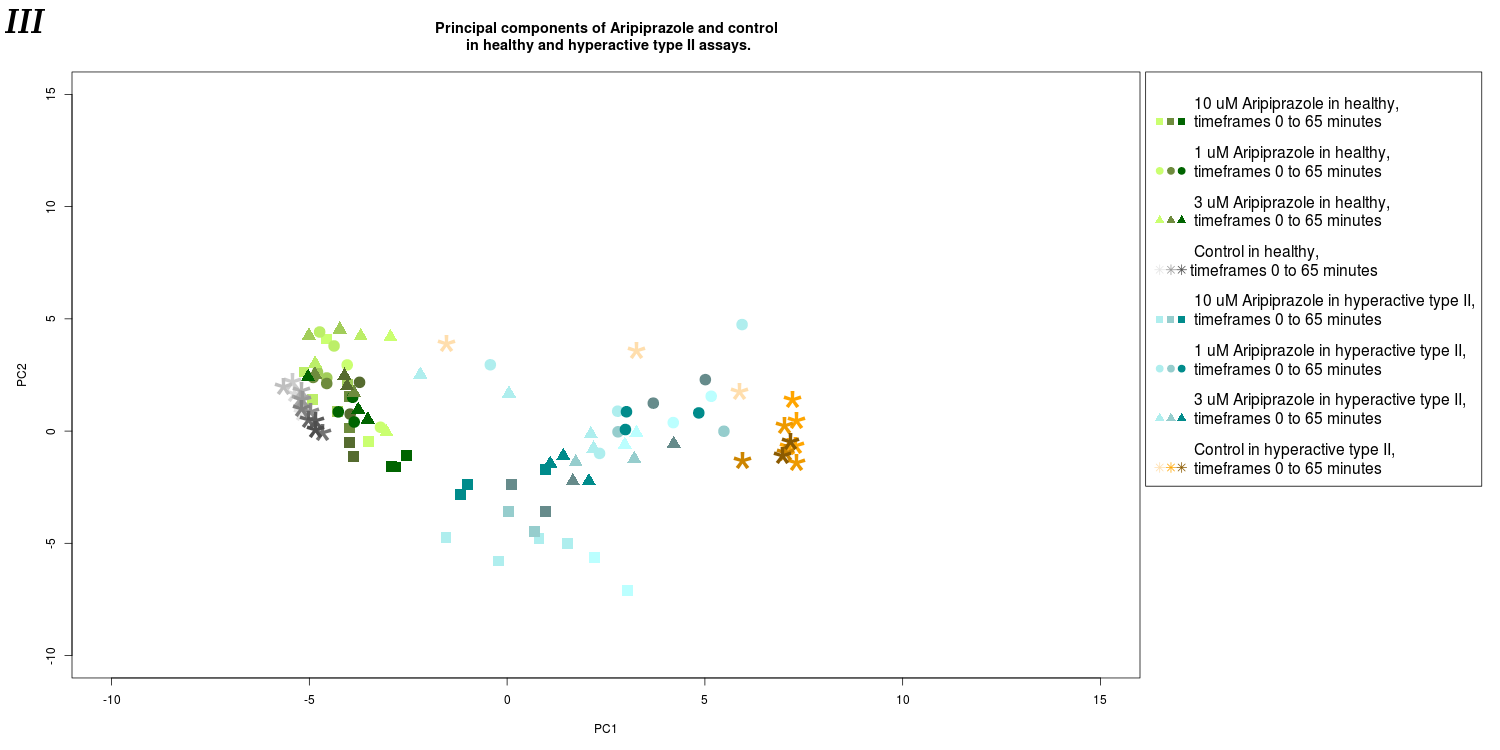
\includegraphics[width=16cm,height=8cm]{Aripiprazole_Control_DarkPTZ_turn_only.png}
\caption{By using the second set of descriptive statistics, the first and second PC of the control in healthy(grey star) and the control in the (\textbf{I})hypoactive, (\textbf{II}) type I hyperactive and (\textbf{III})type II hyperactive control(orange star) along with Aripiprazole in three different dosages(square for a high dose, triangle for a medium dose and a circle for a low dose) in the healthy condition(green) and in the disease induced condition(blue). Colour intensity coded by progress in time.}
\end{center}
\end{figure}
\newpage
% Please add the following required packages to your document preamble:
% \usepackage{multirow}
\begin{table}[h!]\tiny
\centering
\begin{tabular}{|c|c|c|c|}
\hline
                                                    & \begin{tabular}[c]{@{}c@{}}hypoactive\\condition\end{tabular}                &\begin{tabular}[c]{@{}c@{}} type I hyperactive\\condition \end{tabular}              & \begin{tabular}[c]{@{}c@{}}type II hyperactive\\condition\end{tabular}                \\ \hline
\begin{tabular}[c]{@{}c@{}c@{}c@{}c@{}}First 10\\most influential\\descriptive\\statistics\\\end{tabular} & Scoots Proportion                  & Transition ii proportion                  &  E-Bends Proportion Proportion                 \\ \cline{2-4} 
\begin{tabular}[c]{@{}c@{}c@{}c@{}} \\ \\ \\\end{tabular}                                                    & C-Bends Proportion                   & E-Bends Proportion            &  Transition se Proportion      \\ \cline{2-4} 
\begin{tabular}[c]{@{}c@{}c@{}c@{}} \\ \\ \\\end{tabular}                                                     & Transition sss Proportion           & Transition es Proportion            & Transition ee Proportion      \\ \cline{2-4} 
\begin{tabular}[c]{@{}c@{}c@{}c@{}} \\ \\ \\\end{tabular}                                                     & I-bends Proportion            & Transition ee Proportion           &  Transition es Proportion \\ \cline{2-4} 
\begin{tabular}[c]{@{}c@{}c@{}c@{}} \\ \\ \\\end{tabular}                                                     & Transition ss Proportion                   & Transition gg Proportion            & Transition sse Proportion            \\ \cline{2-4} 
 \begin{tabular}[c]{@{}c@{}c@{}c@{}} \\ \\ \\\end{tabular}                                                    & H-bends Proportion                   & Transition se Proportion      & Transition cc Proportion            \\ \cline{2-4} 
\begin{tabular}[c]{@{}c@{}c@{}c@{}} \\ \\ \\\end{tabular}                                                     & Transition cs Proportion            & Transition see Proportion            & Transition ge Proportion            \\ \cline{2-4} 
\begin{tabular}[c]{@{}c@{}c@{}c@{}} \\ \\ \\\end{tabular}                                                     & Transition css Proportion           & Transition ig Proportion           & Transition sc Proportion           \\ \cline{2-4} 
\begin{tabular}[c]{@{}c@{}c@{}c@{}} \\ \\ \\\end{tabular}                                                     & Transition is Proportion            & Transition ssg Proportion &  Transition ses Proportion      \\ \cline{2-4} 
\begin{tabular}[c]{@{}c@{}c@{}c@{}} \\ \\ \\\end{tabular}                                                     & J-bends Proportion                   & Transition sgg Proportion            & Transition eg Proportion           \\ \cline{2-4} 
\begin{tabular}[c]{@{}c@{}c@{}c@{}} \\ \\ \\\end{tabular}                                                     & Transition hs Proportion      & Transition si Proportion           & Transition eee Proportion       \\ \hline
\end{tabular}
\caption{By using the second set of descriptive statistics, the first 10 most correlated descriptive statistics in each of the three disease induced conditions, when comparing to the first five principal components.}
\end{table}

To isolate the variance occurring directly in the turns and turn transitions, the descriptive statistics for the turn and turn transition proportions were extracted per bout length stratum. Stratification will ensure that the turn and turn transition descriptive statistics do not contain variance from the bout length descriptive statistics, but consequentially, it will also drastically increase the number of variables.
\\Plots of the first and second principal components of a PCA, conducted on a set of all descriptive statistics, where the turn and turn transition proportions were stratified in bout length, visually differed from the previous plots, examples shown in Figures 8.1, 8.2 and 8.3, for the hypoactive, type I hyperactive and type II hyperactive condition, respectively. \\First 10 most influential descriptive statistics shown in Table 5.\\Cumulative variance accounted by the first five principal components ranged from approximately 15\% to 22\% with the entire third set of descriptive statistics, while for the set of the first 50 most influential descriptive statistics, the first principal components accounted for approximately 72\% to 90\% of total variance.
\newpage
\begin{figure}[h!]
\begin{center}
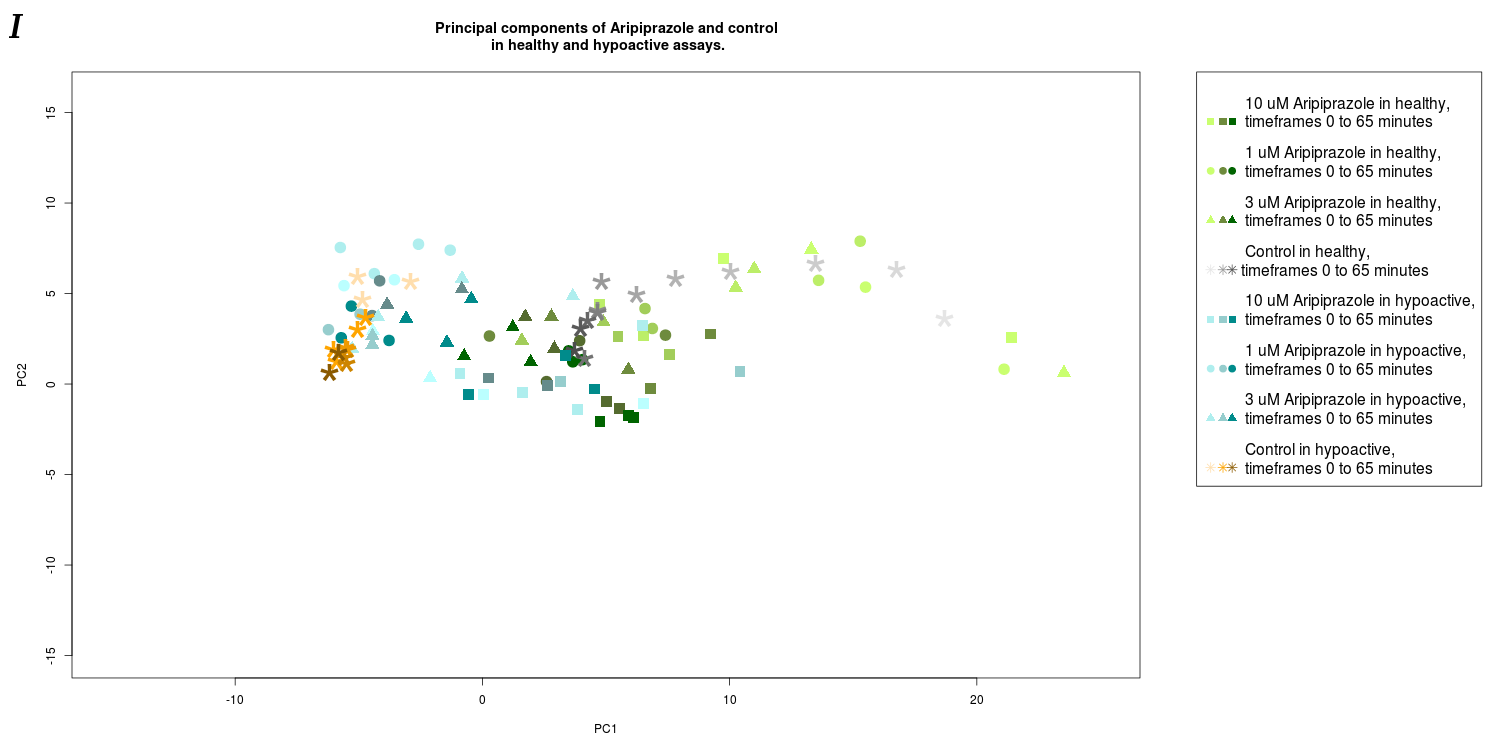
\includegraphics[width=16cm,height=8cm]{Aripiprazole_Control_DarkApoLow_stratified.png}
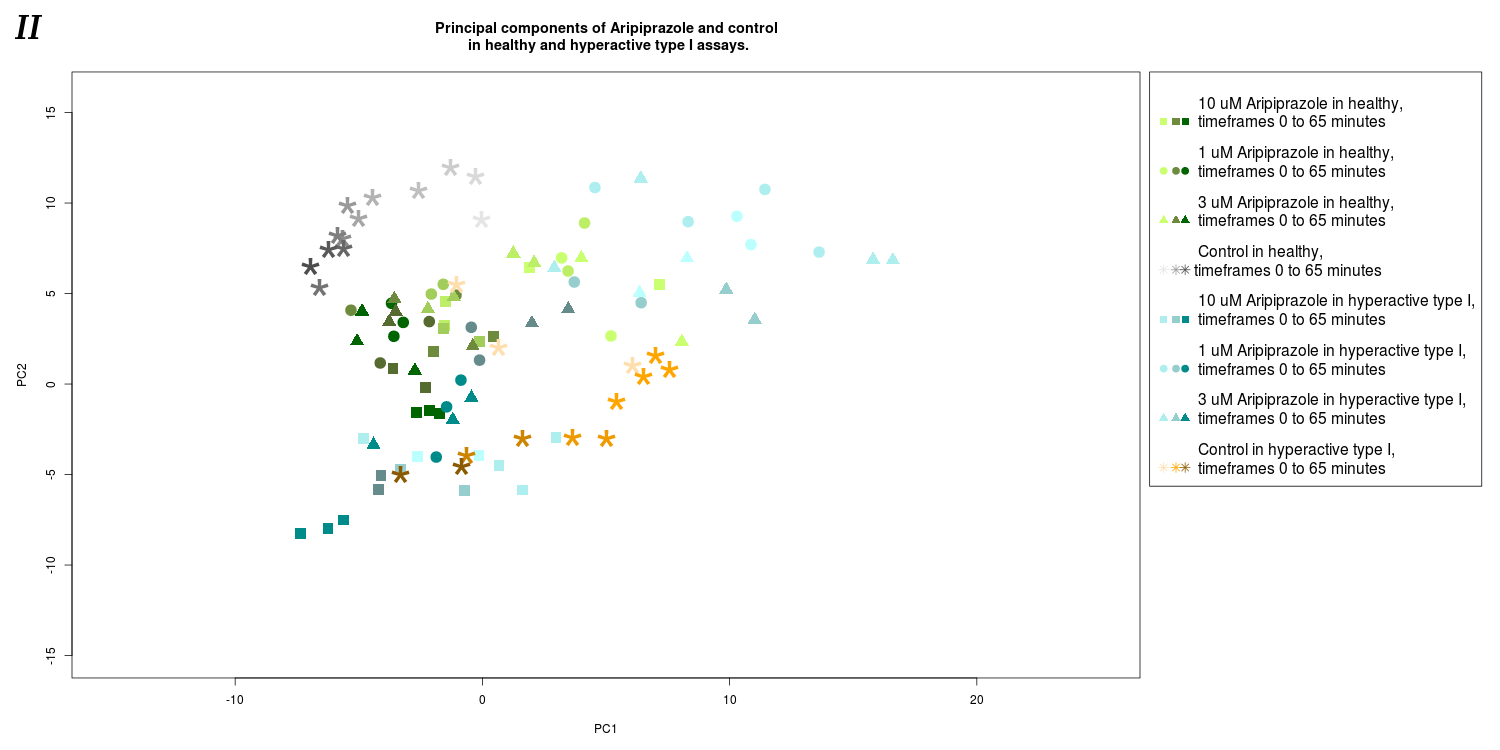
\includegraphics[width=16cm,height=8cm]{Aripiprazole_Control_DarkApoHigh_stratified.png}
\end{center}
\end{figure}

\newpage
\begin{figure}[h!]
\begin{center}
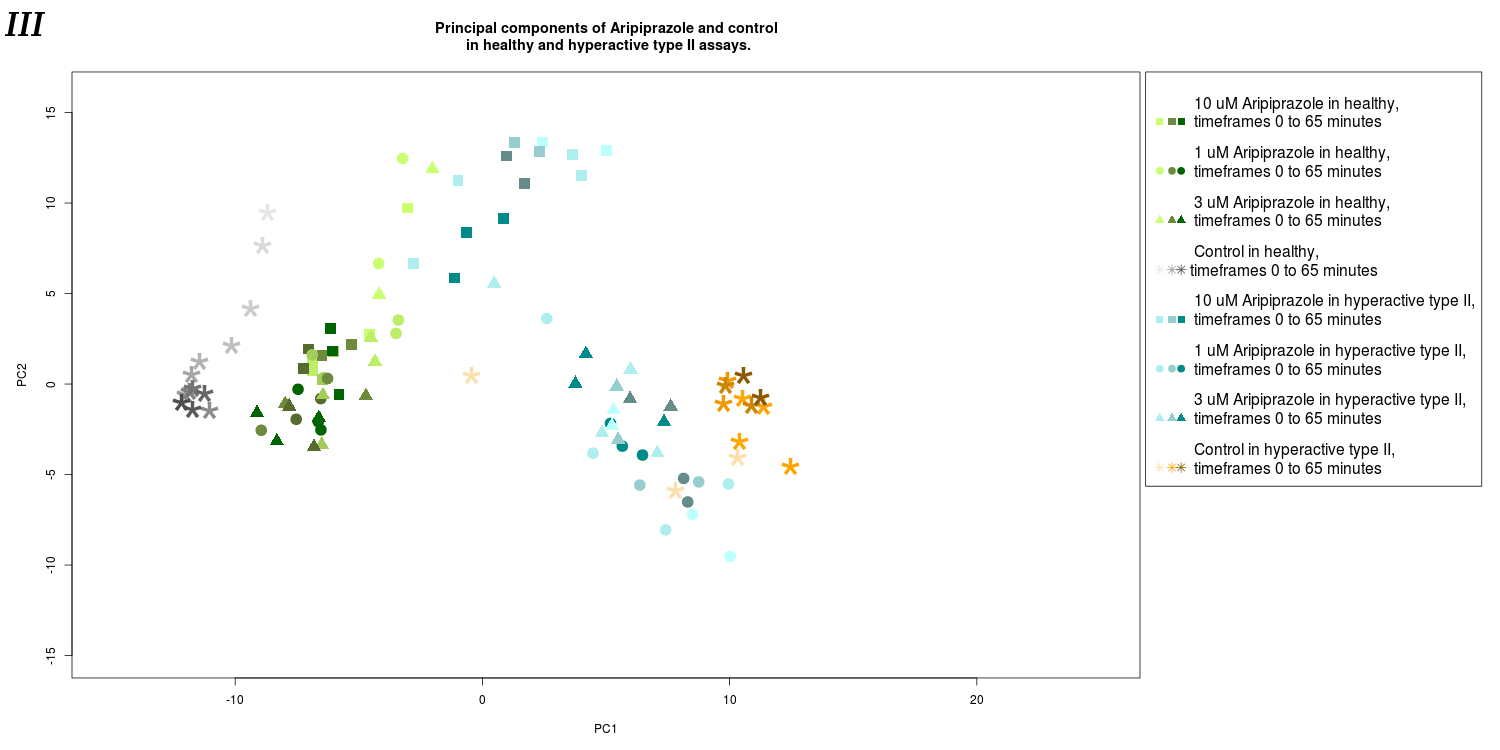
\includegraphics[width=16cm,height=8cm]{Aripiprazole_Control_DarkPTZ_stratified.png}
\caption{By using the third set of descriptive statistics, the first and second PC of the control in healthy(grey star) and the control in the (\textbf{I})hypoactive, (\textbf{II}) type I hyperactive and (\textbf{III})type II hyperactive control(orange star) along with Aripiprazole in three different dosages(square for a high dose, triangle for a medium dose and a circle for a low dose) in the healthy condition(green) and in the disease induced condition(blue). Colour intensity coded by progress in time.}
\end{center}
\end{figure}
\newpage
% Please add the following required packages to your document preamble:
% \usepackage{multirow}
\begin{table}[h!]\tiny
\centering
\begin{tabular}{|c|c|c|c|}
\hline
                                                    & \begin{tabular}[c]{@{}c@{}}hypoactive\\condition\end{tabular}                &\begin{tabular}[c]{@{}c@{}} type I hyperactive\\condition \end{tabular}              & \begin{tabular}[c]{@{}c@{}}type II hyperactive\\condition\end{tabular}                \\ \hline
\begin{tabular}[c]{@{}c@{}c@{}c@{}c@{}}First 10\\most influential\\descriptive\\statistics\\\end{tabular} & Length 6 Plus Transition gs Proportion  &  Length 3 Bout Scoots Proportion  & Length 2 Bout E-Bends Proportion \\ \cline{2-4} 
\begin{tabular}[c]{@{}c@{}c@{}c@{}} \\ \\ \\\end{tabular}                                                     &  Length 5 Transition gs Proportion &  Length 2 Bout Scoots Proportion  &   Length 1 Bout E-Bends Proportion      \\ \cline{2-4} 
\begin{tabular}[c]{@{}c@{}c@{}c@{}} \\ \\ \\\end{tabular}                                                      & Length 3 Transition gs Proportion  &  Length 4 Bout Scoots Proportion  &    Length 3 Bout E-Bends Proportion     \\ \cline{2-4} 
\begin{tabular}[c]{@{}c@{}c@{}c@{}} \\ \\ \\\end{tabular}                                                     & Length 6 Plus Transition gss Proportion &  Length 3 Bout E-Bends Proportion &  Length 2 Bout Scoots Proportion      \\ \cline{2-4} 
\begin{tabular}[c]{@{}c@{}c@{}c@{}} \\ \\ \\\end{tabular}                                                     & TotalBoutCount & Length 6 Plus Bout E-Bends Proportion  &  Length 3 Bout Scoots Proportion      \\ \cline{2-4} 
 \begin{tabular}[c]{@{}c@{}c@{}c@{}} \\ \\ \\\end{tabular}                                                    & Length 5 Transition gss Proportion & Length 5 Bout E-Bends Proportion  &  Length 4 Bout E-Bends Proportion   \\ \cline{2-4} 
\begin{tabular}[c]{@{}c@{}c@{}c@{}} \\ \\ \\\end{tabular}                                                     & Length 4 Transition gs Proportion &  Length 2 Bout E-Bends Proportion &  Length 4 Bout Count Proportion    \\ \cline{2-4} 
\begin{tabular}[c]{@{}c@{}c@{}c@{}} \\ \\ \\\end{tabular}                                                     & Length 3 Transition gss Proportion & Length 4 Bout E-Bends Proportion  &    Length 6 Plus Bout Count Proportion    \\ \cline{2-4} 
\begin{tabular}[c]{@{}c@{}c@{}c@{}} \\ \\ \\\end{tabular}                                                     & Length 4 Transition ss Proportion &  Length 1 Bout E-Bends Proportion &   Length 1 Bout Count Proportion     \\ \cline{2-4} 
\begin{tabular}[c]{@{}c@{}c@{}c@{}} \\ \\ \\\end{tabular}                                                     & Length 5 Transition ss Proportion &  Length 6 Plus Transition se Proportion &   Length 5 Bout Scoots Proportion    \\ \cline{2-4} 
\begin{tabular}[c]{@{}c@{}c@{}c@{}} \\ \\ \\\end{tabular}                                                     & Length 4 Transition gss Proportion&  Length 6 Plus Transition is Proportion  &  Length 5 Bout E-Bends Proportion   \\ \hline
\end{tabular}
\caption{By using the third set of descriptive statistics, the first 10 most correlated descriptive statistics in each of the three disease induced conditions, when comparing to the first five principal components.}
\end{table}
Removing bout count and bout length descriptive statistics from the third set did not change the plots of the first and second principal component. Figures 9.1, 9.2 and 9.3 show examples of plots of the first and second principal component of a PCA, conducted on the fourth set of descriptive statistics with turn and turn transition proportions per bout length only. \\First 10 most influential descriptive statistics are shown in Table 6 and remain almost the same as with the third set of descriptive statistics.\\Cumulative variance accounted by the first five principal components remained in the range from approximately 15\% to 22\% with the entire fourth set of descriptive statistics, while for the set of the first 50 most influential descriptive statistics, the first principal components accounted for approximately 72\% to 90\% of total variance, as when the third set was used.
\newpage
\begin{figure}[h!]
\begin{center}
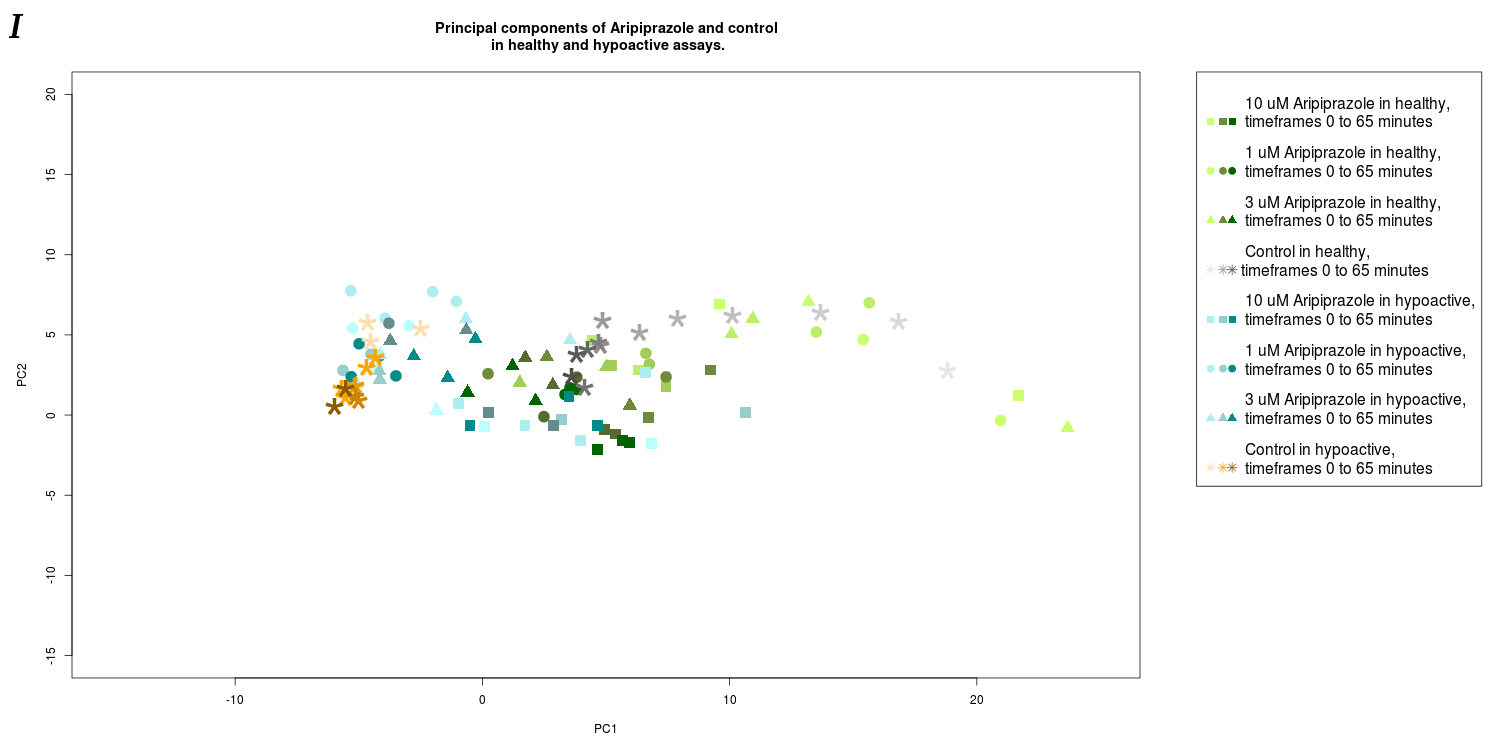
\includegraphics[width=16cm,height=8cm]{Aripiprazole_Control_DarkApoLow_turn_only_stratified.png}
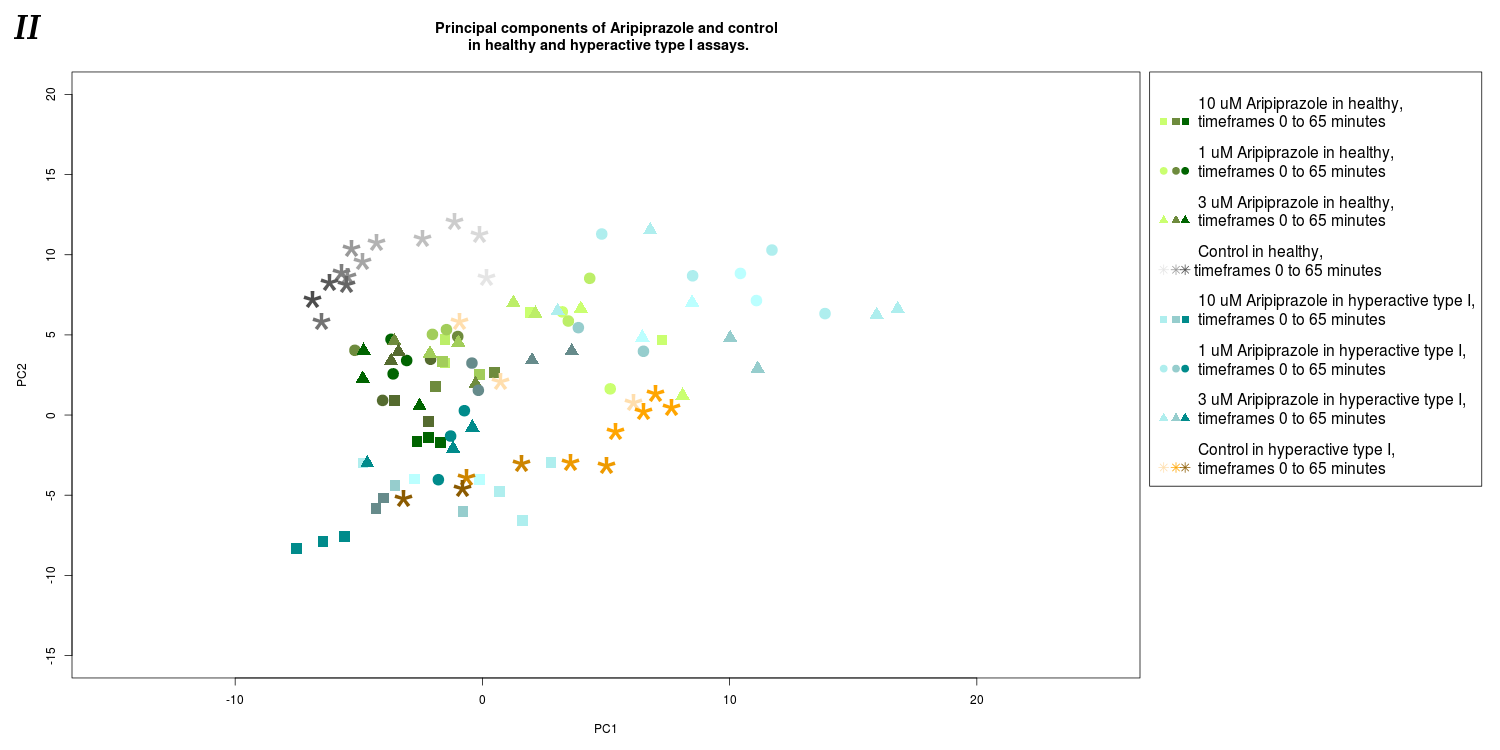
\includegraphics[width=16cm,height=8cm]{Aripiprazole_Control_DarkApoHigh_turn_only_stratified.png}
\end{center}
\end{figure}
\newpage
\begin{figure}[h!]
\begin{center}
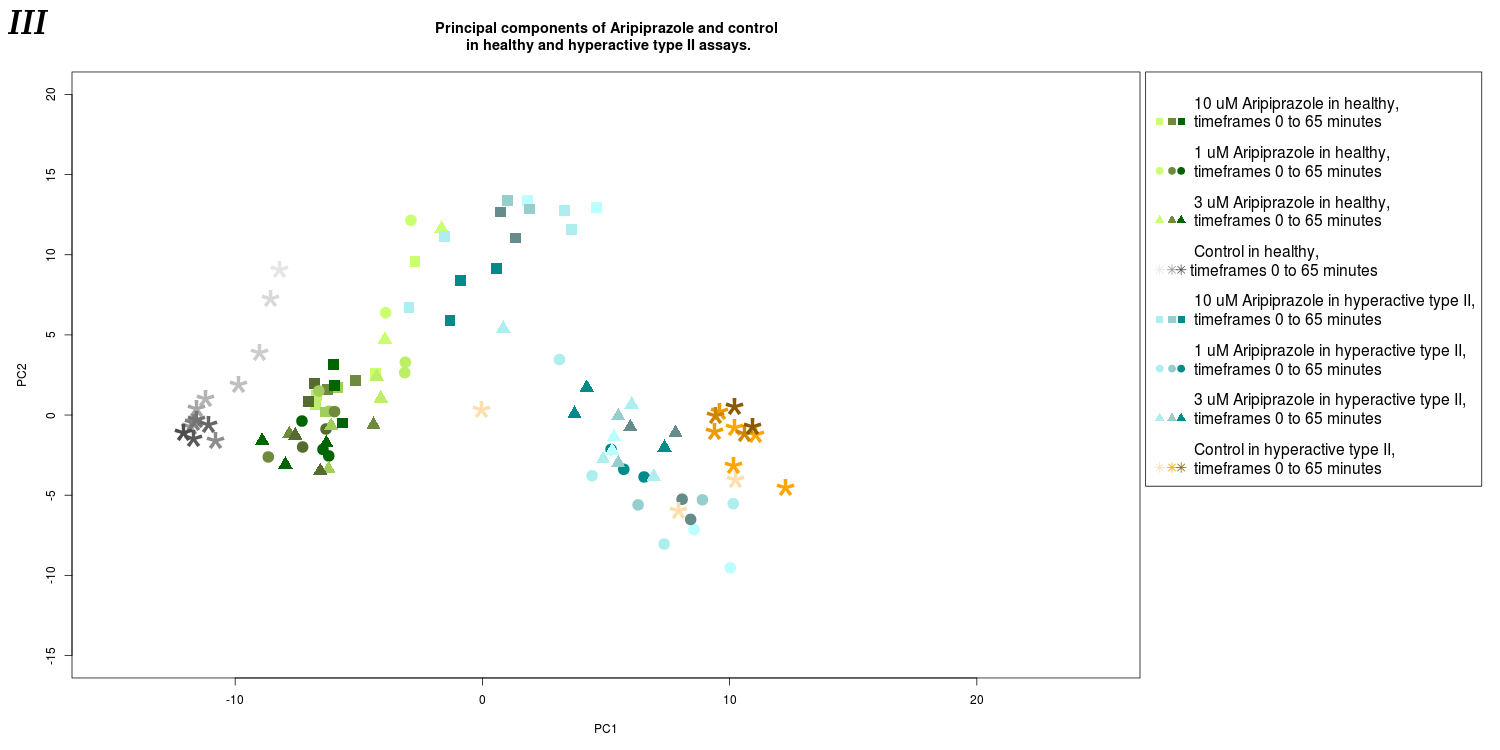
\includegraphics[width=16cm,height=8cm]{Aripiprazole_Control_DarkPTZ_turn_only_stratified.png}
\caption{By using the fourth set of descriptive statistics, the first and second PC of the control in healthy(grey star) and the control in the (\textbf{I})hypoactive, (\textbf{II}) type I hyperactive and (\textbf{III})type II hyperactive control(orange star) along with Aripiprazole in three different dosages(square for a high dose, triangle for a medium dose and a circle for a low dose) in the healthy condition(green) and in the disease induced condition(blue). Colour intensity coded by progress in time.}
\end{center}
\end{figure}
\newpage
% Please add the following required packages to your document preamble:
% \usepackage{multirow}
\begin{table}[h!]\tiny
\centering
\begin{tabular}{|c|c|c|c|}
\hline
                                                    & \begin{tabular}[c]{@{}c@{}}hypoactive\\condition\end{tabular}                &\begin{tabular}[c]{@{}c@{}} type I hyperactive\\condition \end{tabular}              & \begin{tabular}[c]{@{}c@{}}type II hyperactive\\condition\end{tabular}                \\ \hline
\begin{tabular}[c]{@{}c@{}c@{}c@{}c@{}}First 10\\most influential\\descriptive\\statistics\\\end{tabular} & Length 6 Plus Transition gs Proportion  &  Length 3 Bout Scoots Proportion  & Length 2 Bout E-Bends Proportion \\ \cline{2-4} 
\begin{tabular}[c]{@{}c@{}c@{}c@{}} \\ \\ \\\end{tabular}                                                     &  Length 5 Transition gs Proportion &  Length 2 Bout Scoots Proportion  &   Length 1 Bout E-Bends Proportion      \\ \cline{2-4} 
\begin{tabular}[c]{@{}c@{}c@{}c@{}} \\ \\ \\\end{tabular}                                                      & Length 3 Transition gs Proportion  &  Length 4 Bout Scoots Proportion  &    Length 3 Bout E-Bends Proportion     \\ \cline{2-4} 
\begin{tabular}[c]{@{}c@{}c@{}c@{}} \\ \\ \\\end{tabular}                                                     & Length 6 Plus Transition gss Proportion &  Length 3 Bout E-Bends Proportion &  Length 2 Bout Scoots Proportion      \\ \cline{2-4} 
 \begin{tabular}[c]{@{}c@{}c@{}c@{}} \\ \\ \\\end{tabular}                                                    & Length 5 Transition gss Proportion & Length 5 Bout E-Bends Proportion  &  Length 4 Bout E-Bends Proportion   \\ \cline{2-4} 
\begin{tabular}[c]{@{}c@{}c@{}c@{}} \\ \\ \\\end{tabular}                                                     & Length 4 Transition gs Proportion &  Length 2 Bout E-Bends Proportion &  Length 5 Bout Scoots Proportion    \\ \cline{2-4} 
\begin{tabular}[c]{@{}c@{}c@{}c@{}} \\ \\ \\\end{tabular}                                                     & Length 3 Transition gss Proportion & Length 4 Bout E-Bends Proportion  &    Length 6 Plus E-Bends Proportion    \\ \cline{2-4} 
\begin{tabular}[c]{@{}c@{}c@{}c@{}} \\ \\ \\\end{tabular}                                                     & Length 4 Transition ss Proportion &  Length 1 Bout E-Bends Proportion &   Length 5 Bout E-Bends Proportion     \\ \cline{2-4} 
\begin{tabular}[c]{@{}c@{}c@{}c@{}} \\ \\ \\\end{tabular}                                                     & Length 5 Transition ss Proportion &  Length 6 Plus Transition se Proportion &   Length 2 Bout C-Bends Proportion    \\ \cline{2-4} 
\begin{tabular}[c]{@{}c@{}c@{}c@{}} \\ \\ \\\end{tabular}                                                     & Length 4 Transition gss Proportion&  Length 6 Plus Transition is Proportion  &  Length 4 Bout Scoots Proportion   \\ \cline{2-4} 
\begin{tabular}[c]{@{}c@{}c@{}c@{}} \\ \\ \\\end{tabular}                                                     & Length 6 Plus Transition is Proportion & Length 6 Plus Bout E-Bends Proportion  &  Length 3 Bout Scoots Proportion   \\ \hline   
\end{tabular}
\caption{By using the fourth set of descriptive statistics, the first 10 most correlated descriptive statistics in each of the three disease induced conditions, when comparing to the first five principal components.}
\end{table}
\\\\
PCA results were summarized in order to present all compounds at once.\\First, the direction of change in time was plotted for all compounds, for each of the three dosages. Figures 10.1, 10.2 and 10.3 show an example of the summarized plots for the type II hyperactive condition, using the third set of descriptive statistics with respect to the direction in time, for the low, medium and high dosage respectively. All summarized plots, showing the direction of change in time for all three disease induced conditions, all four descriptive statisitcs and all three dosages are shown in Appendix C.3.
\newpage
\begin{figure}[h!]
\begin{center}
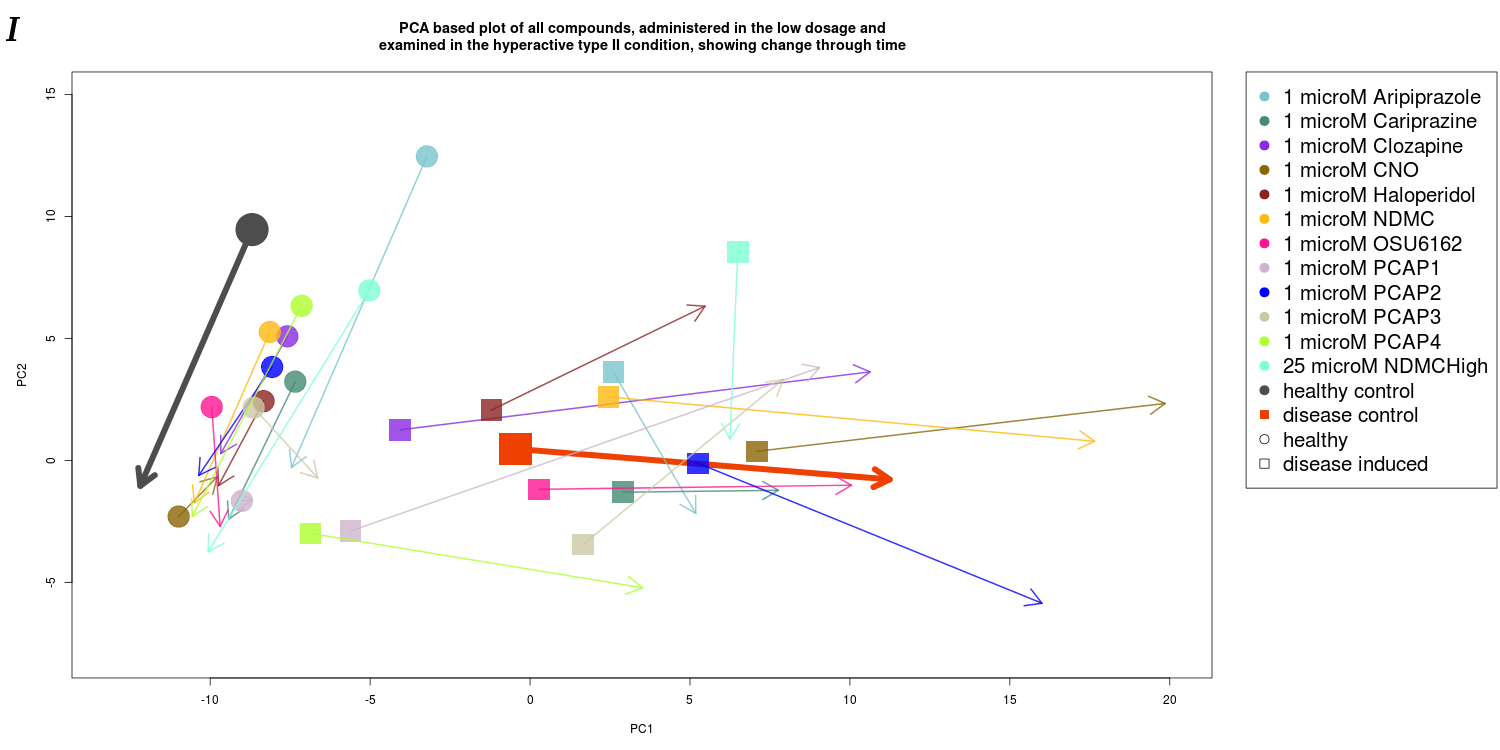
\includegraphics[width=16cm,height=8cm]{All_together_1_microM_DarkPTZ_in_time_set3.png}
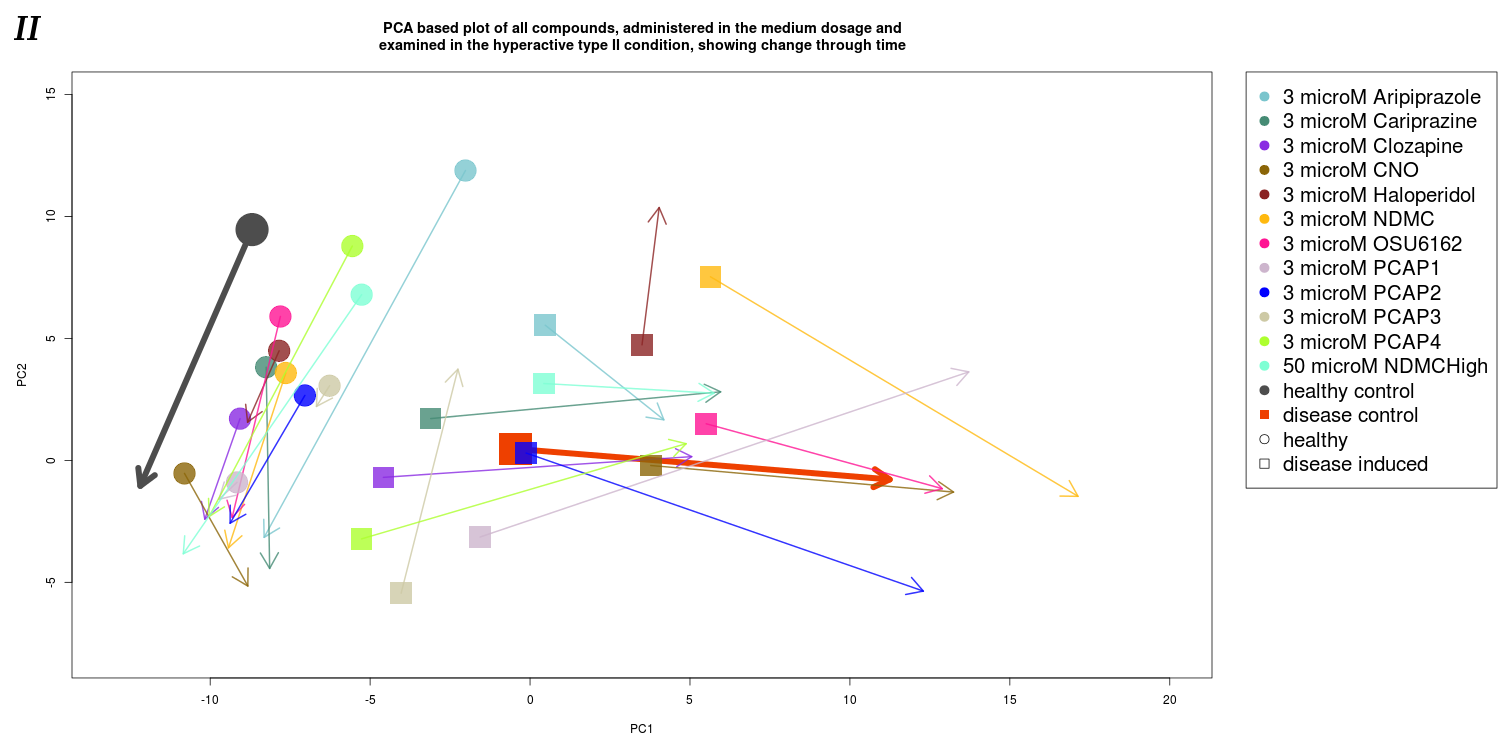
\includegraphics[width=16cm,height=8cm]{All_together_3_microM_DarkPTZ_in_time_set3.png}
\end{center}
\end{figure}
\newpage
\begin{figure}[h!]
\begin{center}
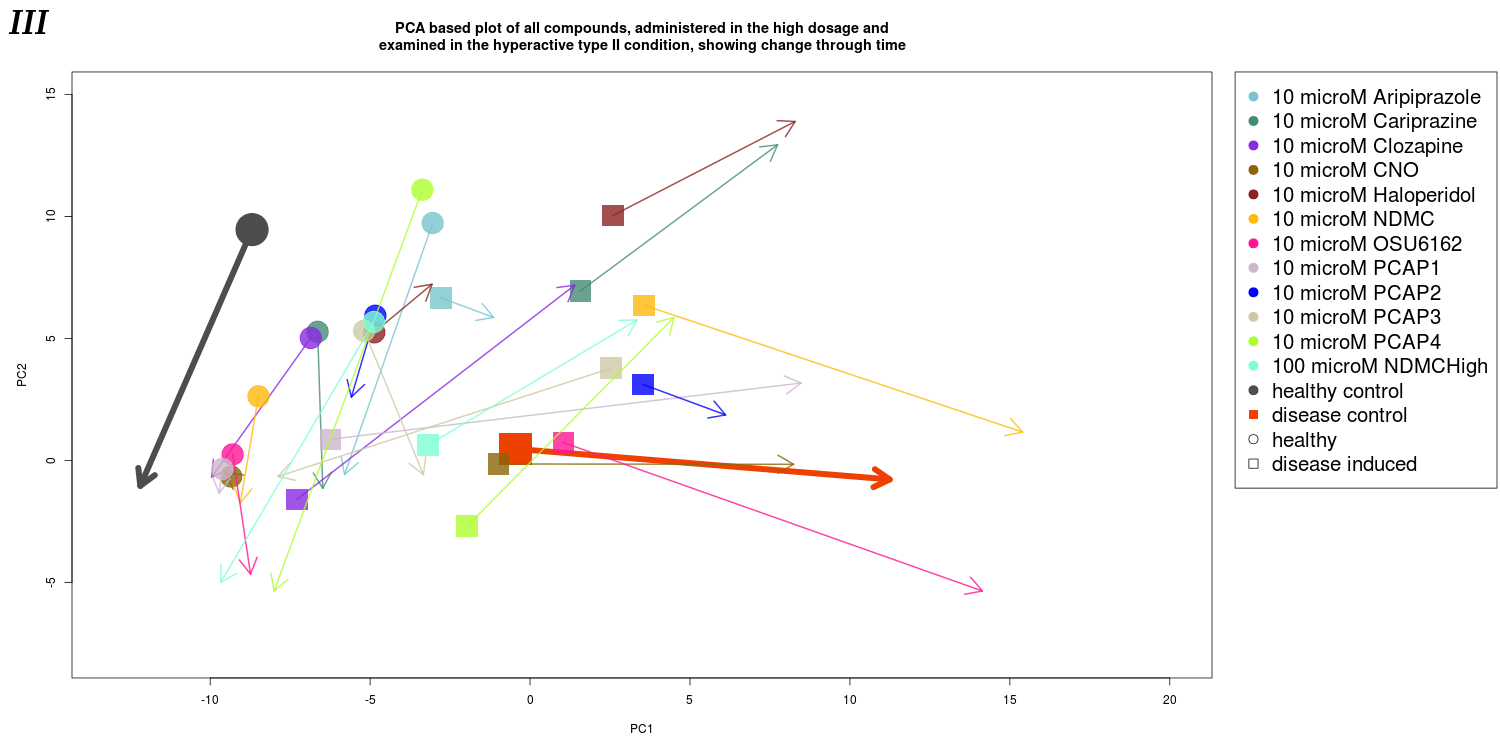
\includegraphics[width=16cm,height=8cm]{All_together_10_microM_DarkPTZ_in_time_set3.png}
\caption{A summarized plot of the PCA results for the type II hyperactive condition, using the third set of descriptive statistics and showing the direction of change in time when administrating a (\textbf{I})low, a (\textbf{II})medium and a (\textbf{III})high dosage of compounds.}
\end{center}
\end{figure}

\\Second, the direction of change in dosage was plotted for all compounds, averaged over all thirteen timeframes. Figures 11.1, 11.2 and 11.3 show an example of the summarized plots, showing the direction of change in dosage, for the hypoactive, type I hyperactive and the type II hyperactive condition, using the third set of descriptive statistics. All summarized plots, showing the direction of change in dosage for all three disease induced conditions and all four descriptive statisitcs are shown in Appendix C.4.
\newpage
\begin{figure}[h!]
\begin{center}
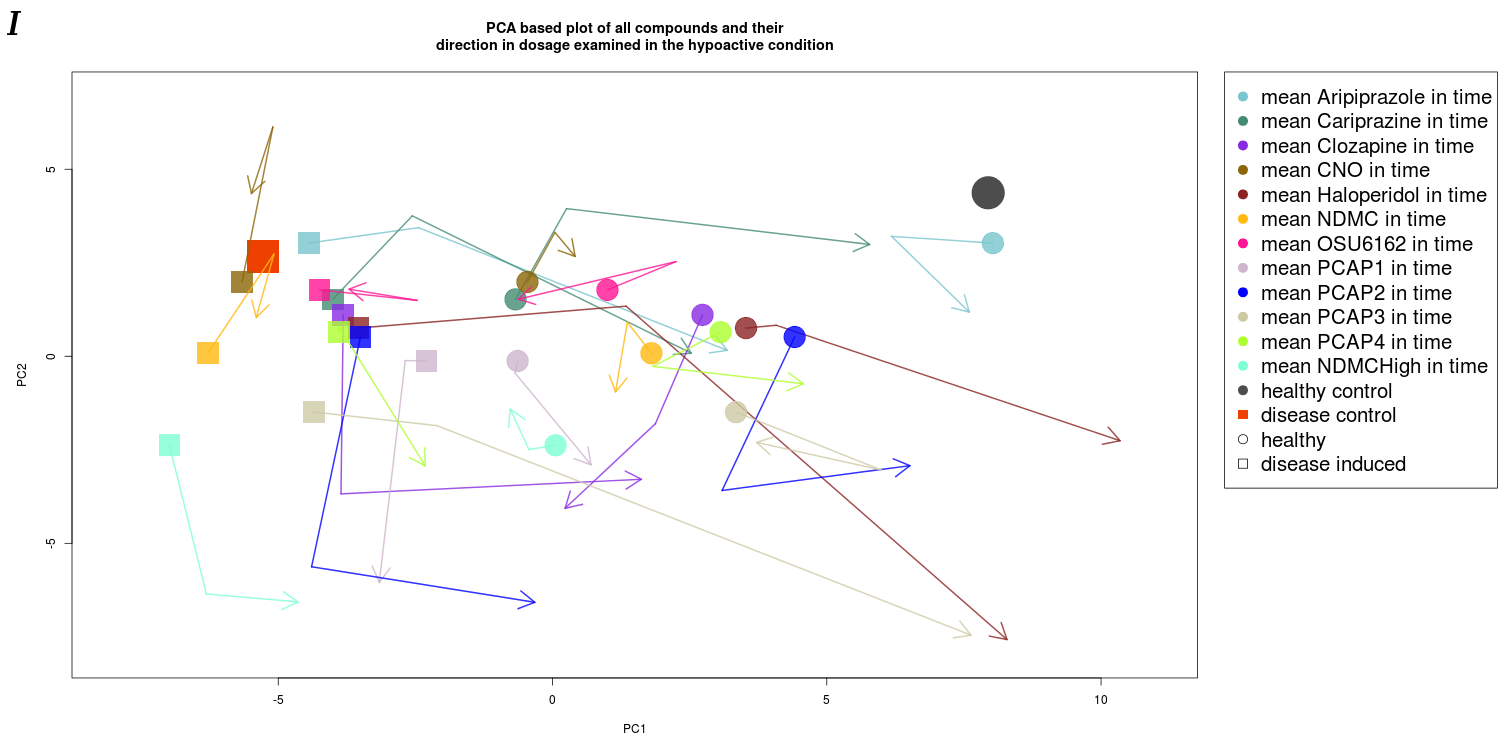
\includegraphics[width=16cm,height=8cm]{All_together_doses_DarkApoLowset3.png}
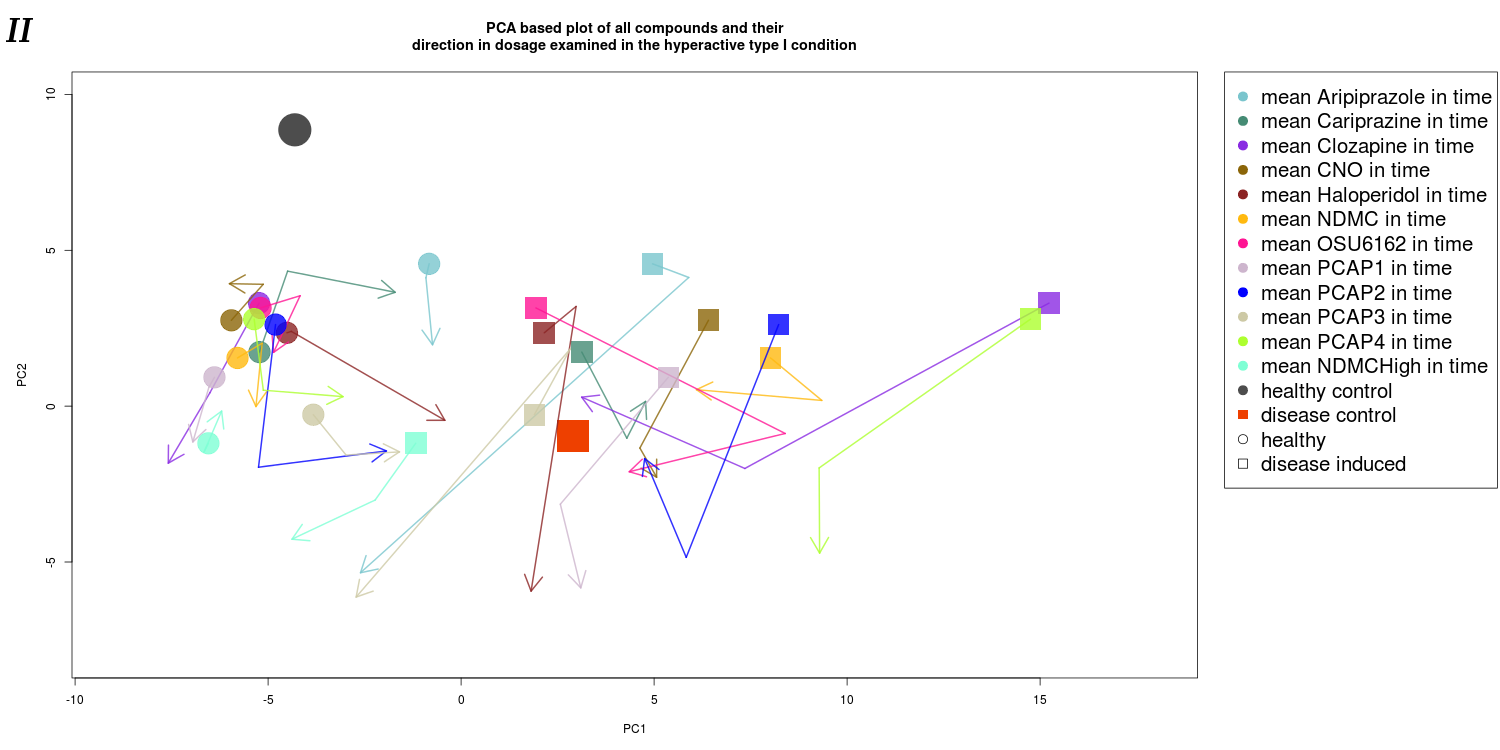
\includegraphics[width=16cm,height=8cm]{All_together_doses_DarkApoHighset3.png}
\end{center}
\end{figure}
\newpage
\begin{figure}[h!]
\begin{center}
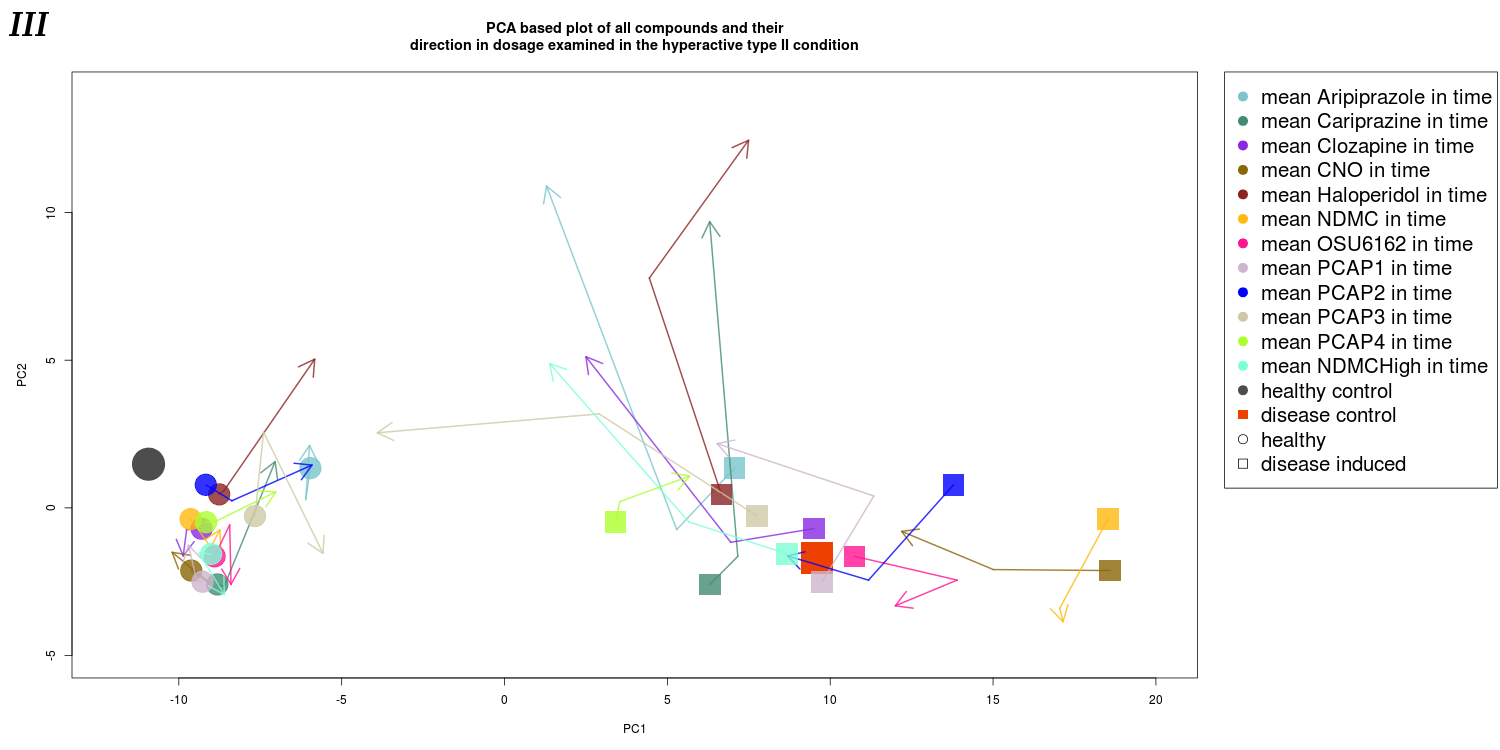
\includegraphics[width=16cm,height=8cm]{All_together_doses_DarkPTZset3.png}
\caption{A summarized plot of the PCA results for the (\textbf{I})hypoactive, (\textbf{II})type I hyperactive and (\textbf{III})type II hyperactive condition, using the third set of descriptive statistics, showing the direction of change in dosage.}
\end{center}
\end{figure}


\\By further exploring the results of PCA, compound effects were explored based on the proximity to the healthy control group in each time frame. Using the first set of descriptive statistics, mean, standard deviation(SD), minimum(MIN) and maximum(MAX) of the Euclidean distances, representing the proximity over all time frames, are shown for the first three and last three closest compounds given to the healthy and hypoactive larvae in Table 7 and 8, respectively. Full list of ranked compounds, for all three disease induced conditions and all four sets of descriptive statistics is shown in Appendix C.5.
\begin{table}[h!]\tiny
\centering
\begin{tabular}{|c|c|c|c|c|}
\hline
first three          & mean & SD   & MIN  & MAX   \\ \hline
OSU6162 1microM       & 1.20  & 0.47 & 0.46 & 1.83  \\ \hline
Clozapine 1microM     & 1.44 & 0.50  & 0.83 & 2.77  \\ \hline
CNO 1microM           & 1.60  & 0.59 & 0.60  & 2.67  \\ \hline
last three           & \multicolumn{4}{c|}{}      \\ \hline
PCAP3 10microM      & 5.29 & 2.79 & 0.97 & 10.73 \\ \hline
PCAP3 1microM       & 5.87 & 5.39 & 0.88 & 18.89 \\ \hline
PCAP2 10microM        & 6.70  & 3.56 & 2.20  & 12.88 \\ \hline
\end{tabular}
\caption{Using the first set of the descriptive statistics of the hypoactive condition, the first and last three closest compounds to the healthy control, when administered to the healthy larvae, based on the Euclidean distances between the first five principal components through all time frames.}
\end{table}
\newpage
\begin{table}[h!]\tiny
\centering
\begin{tabular}{|c|c|c|c|c|}
\hline
first three           & mean & SD   & MIN  & MAX   \\ \hline
Haloperidol 3microM   & 1.99  & 0.93  & 0.94 & 3.64  \\ \hline
Cariprazine 10microM  & 2.54  & 1.09  & 0.8  & 5.14  \\ \hline
PCAP4 1microM       & 3.38  & 1.58  & 1.52 & 6.39  \\ \hline
last three            & \multicolumn{4}{c|}{}      \\ \hline
PCAP1 1microM         & 9.65  & 16.33 & 2.89 & 63.85 \\ \hline
Haloperidol 10microM  & 10.92 & 5.61  & 5.77 & 22.48 \\ \hline
PCAP3 10microM      & 11.43 & 5.04  & 6.19 & 26.25 \\ \hline
\end{tabular}
\caption{Using the first set of the descriptive statistics of the hypoactive condition, the first and last three closest compounds to the healthy control, when administered to the hypoactive larvae, based on the Euclidean distances between the first five principal components through all time frames.}
\end{table}
Haloperidol, administered in 3 $\mu$M appears to be efficient, aiding hypoactive larvae to behave as the healthy larvae, while not having a substantial effect on the healthy larvae. This can be seen in the plot of the first and second principal component, where it is also apparent that a higher dose of Haloperidol, at 10 $\mu$M, will have a visible effect on the healthy larvae, while the hypoactive larvae do not behave as the healthy control, an example is shown in Figure 12.
\begin{figure}[h!]
\begin{center}
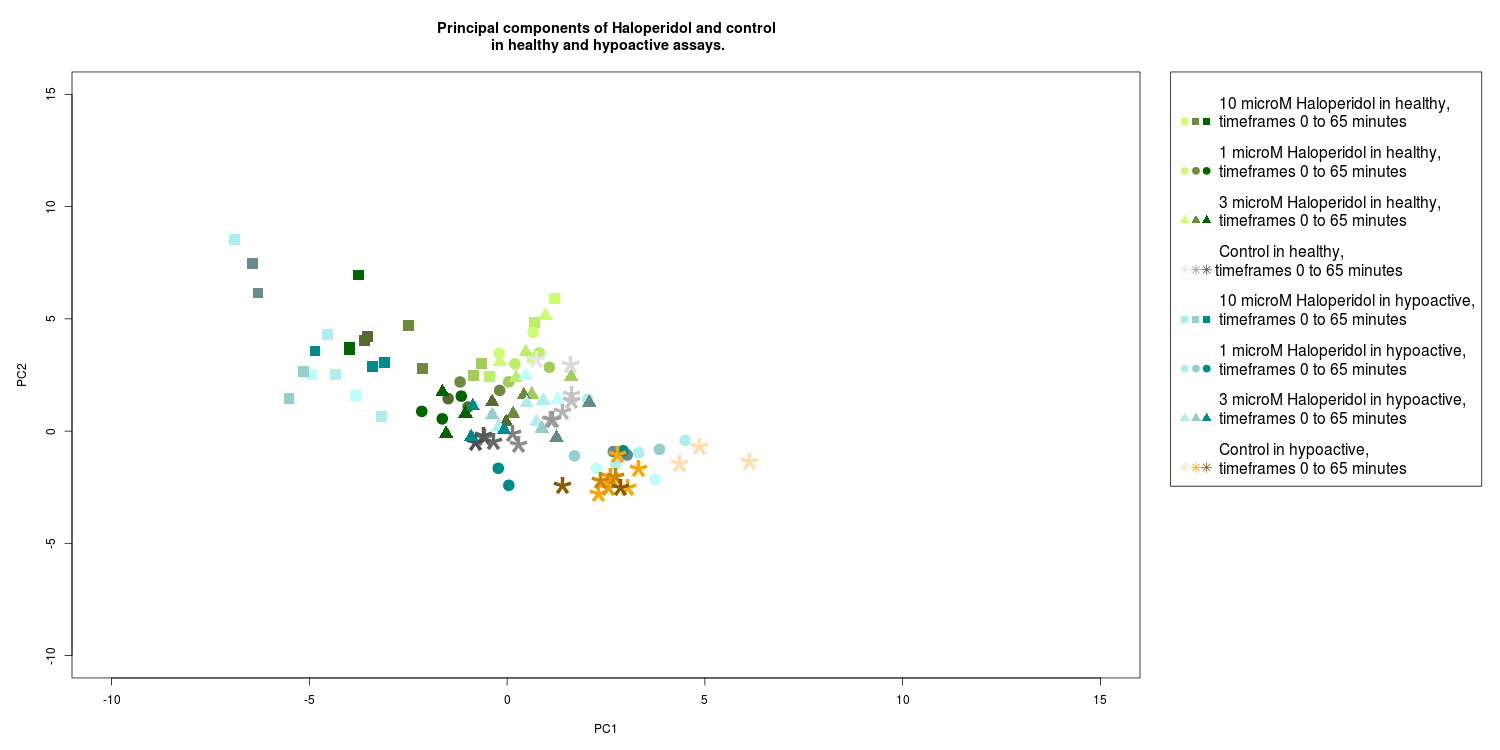
\includegraphics[width=16cm,height=8cm]{Haloperidol_Control_DarkApoLow.png}
\caption{By using the first set of descriptive statistics, the first and second PC of the control in healthy(grey star) and the control in hypoactive(orange star) along with Haloperidol, administered in three different dosages(square for a high dose, triangle for a medium dose and a circle for a low dose) in the healthy condition(green) and in the hypoactive condition(blue). Colour intensity coded by progress in time.}
\end{center}
\end{figure}
\newpage
Results of compound ranking are slightly different, when using the second set of descriptive statistics, although Haloperidol at a 3 $\mu$M dosage is still the closest and at a 10 $\mu$M dosage, it is the furthest. Mean, standard deviation(SD), minimum(MIN) and maximum(MAX) of the Euclidean distances, representing the proximity over all time frames, are shown for the first three and last three closest compounds given to the healthy and hypoactive larvae in Table 9 and 10, respectively.
\begin{table}[h!]\tiny
\centering
\begin{tabular}{|c|c|c|c|c|}
\hline
first three          & mean & SD   & MIN  & MAX   \\ \hline
OSU6162 1 microM       & 1.06 & 0.42 & 0.39 & 1.66  \\ \hline
Clozapine 1 microM     & 1.30  & 0.44 & 0.68 & 2.43  \\ \hline
NDMC 3 microM          & 1.48 & 0.67 & 0.49 & 2.66  \\ \hline
last three           & \multicolumn{4}{c|}{}      \\ \hline
PCAP3 10 microM      & 5.16 & 3.06 & 0.85 & 11.33 \\ \hline
Haloperidol 10 microM  & 5.19 & 2.80  & 1.00    & 12.43 \\ \hline
PCAP2 10 microM        & 6.11 & 3.75 & 1.22 & 12.45 \\ \hline
\end{tabular}
\caption{Using the second set of the descriptive statistics of the hypoactive condition, the first and last three closest compounds to the healthy control, when administered to the healthy larvae, based on the Euclidean distances between the first five principal components through all time frames.}
\end{table}
\begin{table}[h!]\tiny
\centering
\begin{tabular}{|c|c|c|c|c|}
\hline
first three          & mean & SD    & MIN  & MAX   \\ \hline
Haloperidol 3microM   & 1.87  & 0.83  & 0.79 & 3.47  \\ \hline
Cariprazine 10microM  & 2.56  & 1.16  & 0.95 & 5.43  \\ \hline
PCAP4 3microM       & 2.86  & 1.17  & 1.3  & 5.43  \\ \hline
last three           & \multicolumn{4}{c|}{}       \\ \hline
PCAP1 1microM         & 9.29  & 16.42 & 2.81 & 63.81 \\ \hline
Haloperidol 10microM  & 10.72 & 5.59  & 4.84 & 22.47 \\ \hline
PCAP3 10microM      & 10.80  & 5.22  & 5.68 & 26.20  \\ \hline
\end{tabular}
\caption{Using the second set of the descriptive statistics of the hypoactive condition, the first and last three closest compounds to the healthy control, when administered to the hypoactive larvae, based on the Euclidean distances between the first five principal components through all time frames.}
\end{table}
\\
Similar as when using the second set of descriptive statistics, when using the third and fourth set of descriptive statistics, the results are slightly different, while Haloperidol at a 3 $\mu$M dosage is still in the top three closest and at a 10 $\mu$M dosage, it is in the top three furthest.
\\
The results of compound ranking, in their effect on the healthy control larvae, was slightly different when using the PCA results from a set of descriptive statistics combined with the type I hyperactive or with the type II hyperactive condition, compared to the hypoactive condition, due to a different amount of contributed variation.
\\Haloperidol at a 3 $\mu$M dosage was also efficient when administered to the type I hyperactive larvae, while at a 10 $\mu$M dosage it was closer to the behaviour of the healthy control larvae, compared to when administered to the hypoactive larvae at the same dosage. Using the first set of descriptive statistics, mean, standard deviation(SD), minimum(MIN) and maximum(MAX) of the Euclidean distances, representing the proximity over all time frames, are shown for the first three and last three closest compounds given to the healthy and type I hyperactive larvae in Table 11 and 12, respectively.
\begin{table}[h!]\tiny
\centering
\begin{tabular}{|c|c|c|c|c|}
\hline
first three         & mean & SD   & MIN  & MAX  \\ \hline
OSU6162 1microM     & 1.35 & 0.58 & 0.47 & 2.60  \\ \hline
Clozapine 1microM   & 1.57 & 0.76 & 0.68 & 2.87 \\ \hline
Haloperidol 3microM & 1.61 & 0.49 & 0.95 & 2.35 \\ \hline
last three          & \multicolumn{4}{c|}{}     \\ \hline
PCAP2 3microM       & 4.79 & 1.89 & 1.04 & 7.20  \\ \hline
PCAP2 10microM      & 5.28 & 2.08 & 1.55 & 8.42 \\ \hline
PCAP3 10microM    & 5.42 & 2.37 & 0.99 & 8.73 \\ \hline
\end{tabular}
\caption{Using the first set of the descriptive statistics of the type I hyperactive condition, the first and last three closest compounds to the healthy control, when administered to the healthy larvae, based on the Euclidean distances between the first five principal components through all time frames.}
\end{table}
\begin{table}[h!]\tiny
\centering
\begin{tabular}{|c|c|c|c|c|}
\hline
first three          & mean  & SD    & MIN  & MAX   \\ \hline
NDMCHigh 25microM    & 4.49  & 0.99  & 2.49 & 5.94  \\ \hline
Haloperidol 3microM  & 5.04  & 1.29  & 3.11 & 7.75  \\ \hline
PCAP3 3microM      & 5.06  & 1.68  & 2.53 & 7.64  \\ \hline
last three           & \multicolumn{4}{c|}{}        \\ \hline
Clozapine 1microM    & 12.44 & 2.54  & 8.78 & 16.55 \\ \hline
PCAP4 1microM      & 13.42 & 3.93  & 7.52 & 18.43 \\ \hline
Cariprazine 10microM & 15.45 & 12.78 & 5.34 & 46.50  \\ \hline
\end{tabular}
\caption{Using the first set of the descriptive statistics of the type I hyperactive condition, the first and last three closest compounds to the healthy control, when administered to the type I hyperactive larvae, based on the Euclidean distances between the first five principal components through all time frames.}
\end{table}
\\\\When investigating the proximity to the type I hyperactive condition, compound PCAP3 appeared to induce a similar behaviour, as the dosage increased. A plot of the first and second principal component showing the proximity of PCAP3 to the healthy and the type I hyperactive control larvae in Figure 13.1.\\
When exploring PCA results using descriptive statistics from the type II hyperactive condition, compounds PCAP2, Haloperidol and PCAP3, all in higher doses, had a substantial effect on the healthy larvae, being in the top furthest compounds away from the healthy control group, while being in top closest to the type II hyperactive control group, although PCAP3, when administered along with PTZ, was then in the top closest to the healthy control group, example shown in Figure 13.2.
\newpage
\begin{figure}[h!]
\begin{center}
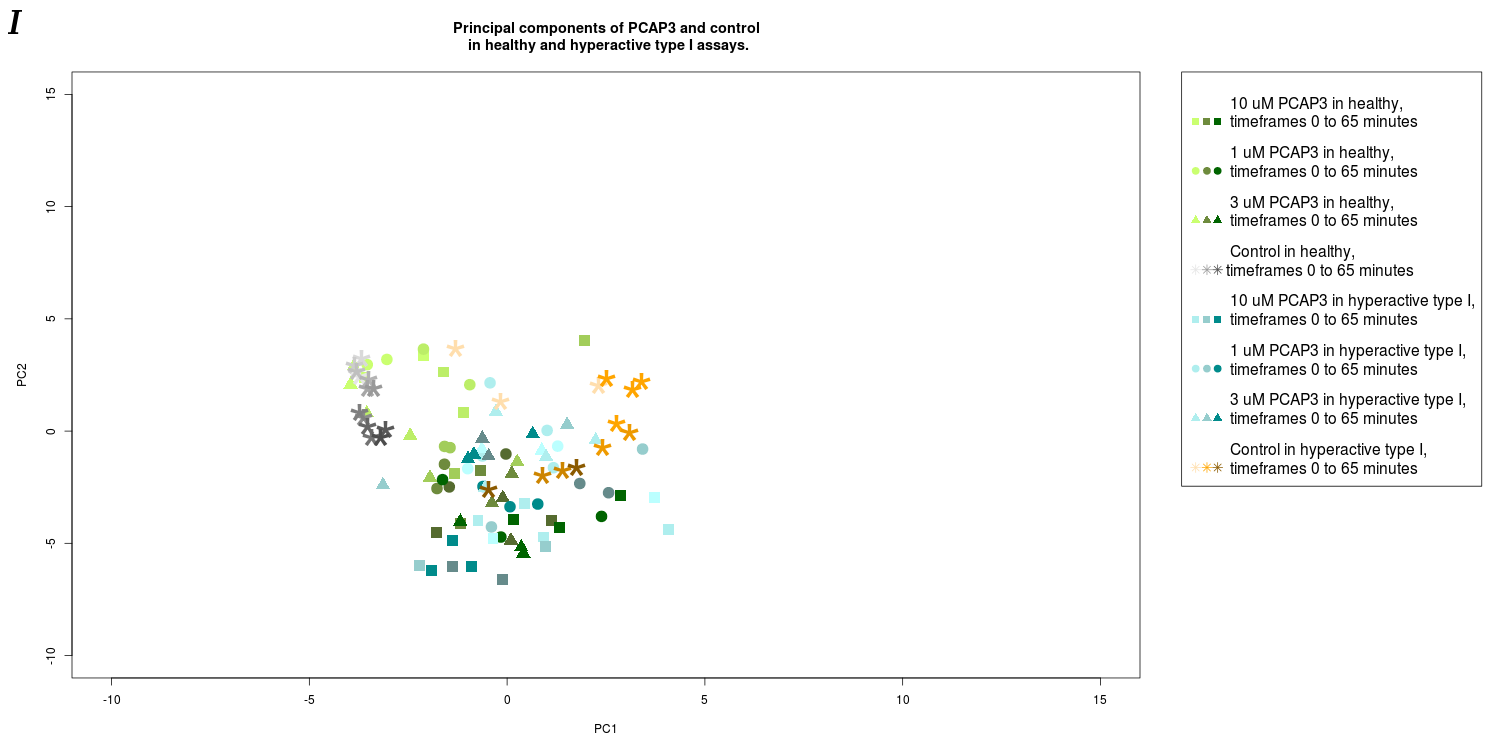
\includegraphics[width=16cm,height=8cm]{PCAP814_Control_DarkApoHigh.png}
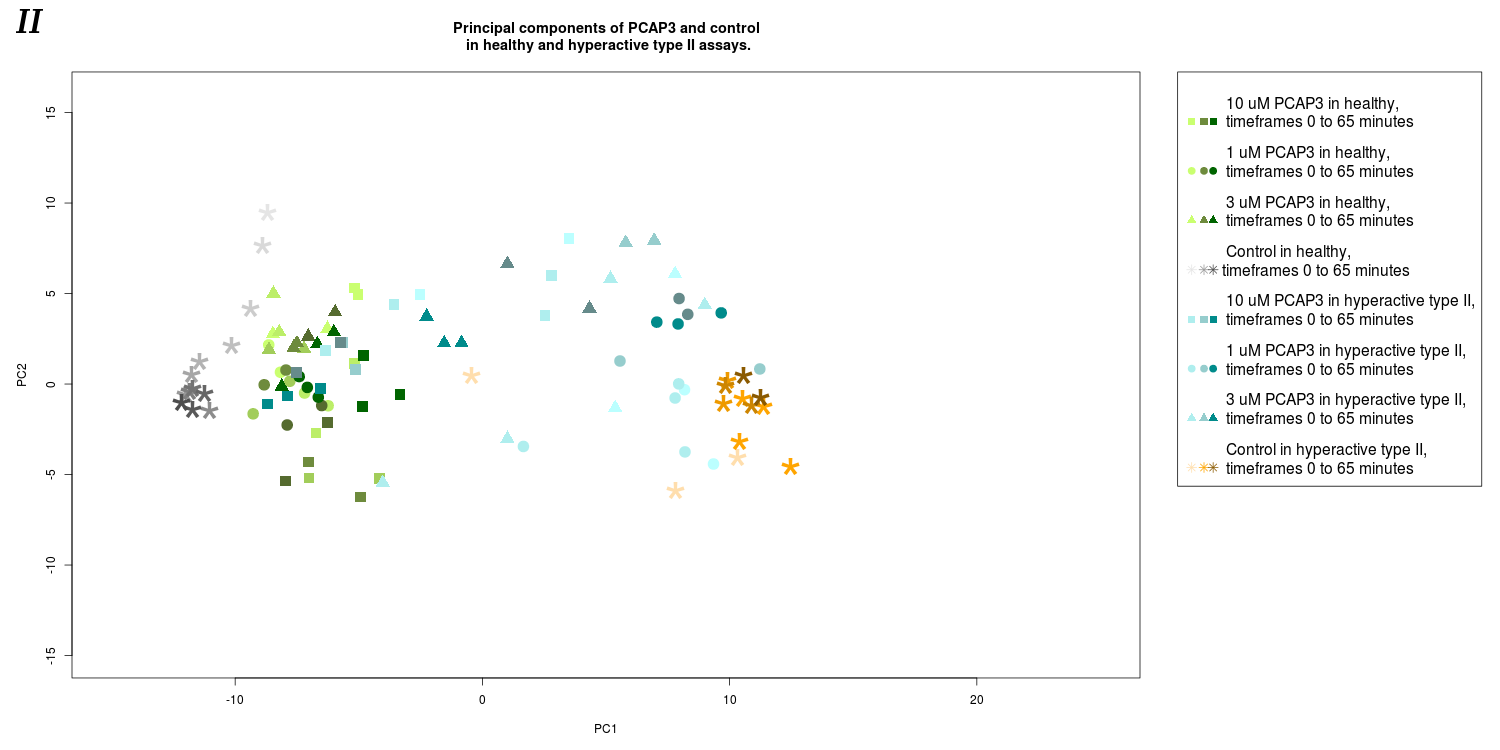
\includegraphics[width=16cm,height=8cm]{PCAP814_Control_DarkPTZ_stratified.png}
\caption{By using the (\textbf{I})first and (\textbf{II})third set of descriptive statistics, the first and second PC of the control in healthy(grey star) and the control in (\textbf{I})type I hyperactive and (\textbf{II})type II hyperactive condition(orange star) along with PCAP3, administered in three different dosages(square for a high dose, triangle for a medium dose and a circle for a low dose) in the healthy condition(green) and in the disease induced condition(blue). Colour intensity coded by progress in time.}
\end{center}
\end{figure}

\newpage
Euclidean distances between the first five principal components were used to construct distance trees, in order to visualise circular cladograms, having experimental groups as leaves, which were colour-coded appropriately. Cladograms were visualised for all three disease induced conditions, using PCA results based on the four different sets of descriptive statistics. Examples of circular cladograms, constructed based on the first five principal components of a PCA using the first set of descriptive statistics, for the hypoactive, type I hyperactive and type II hyperactive condition in Figure 15, Figure 16 and Figure 17, respectively. All circular cladograms, constructed based on Euclidean distances between the principal components, in Appendix C.6. 
\begin{figure}[h!]
\begin{center}
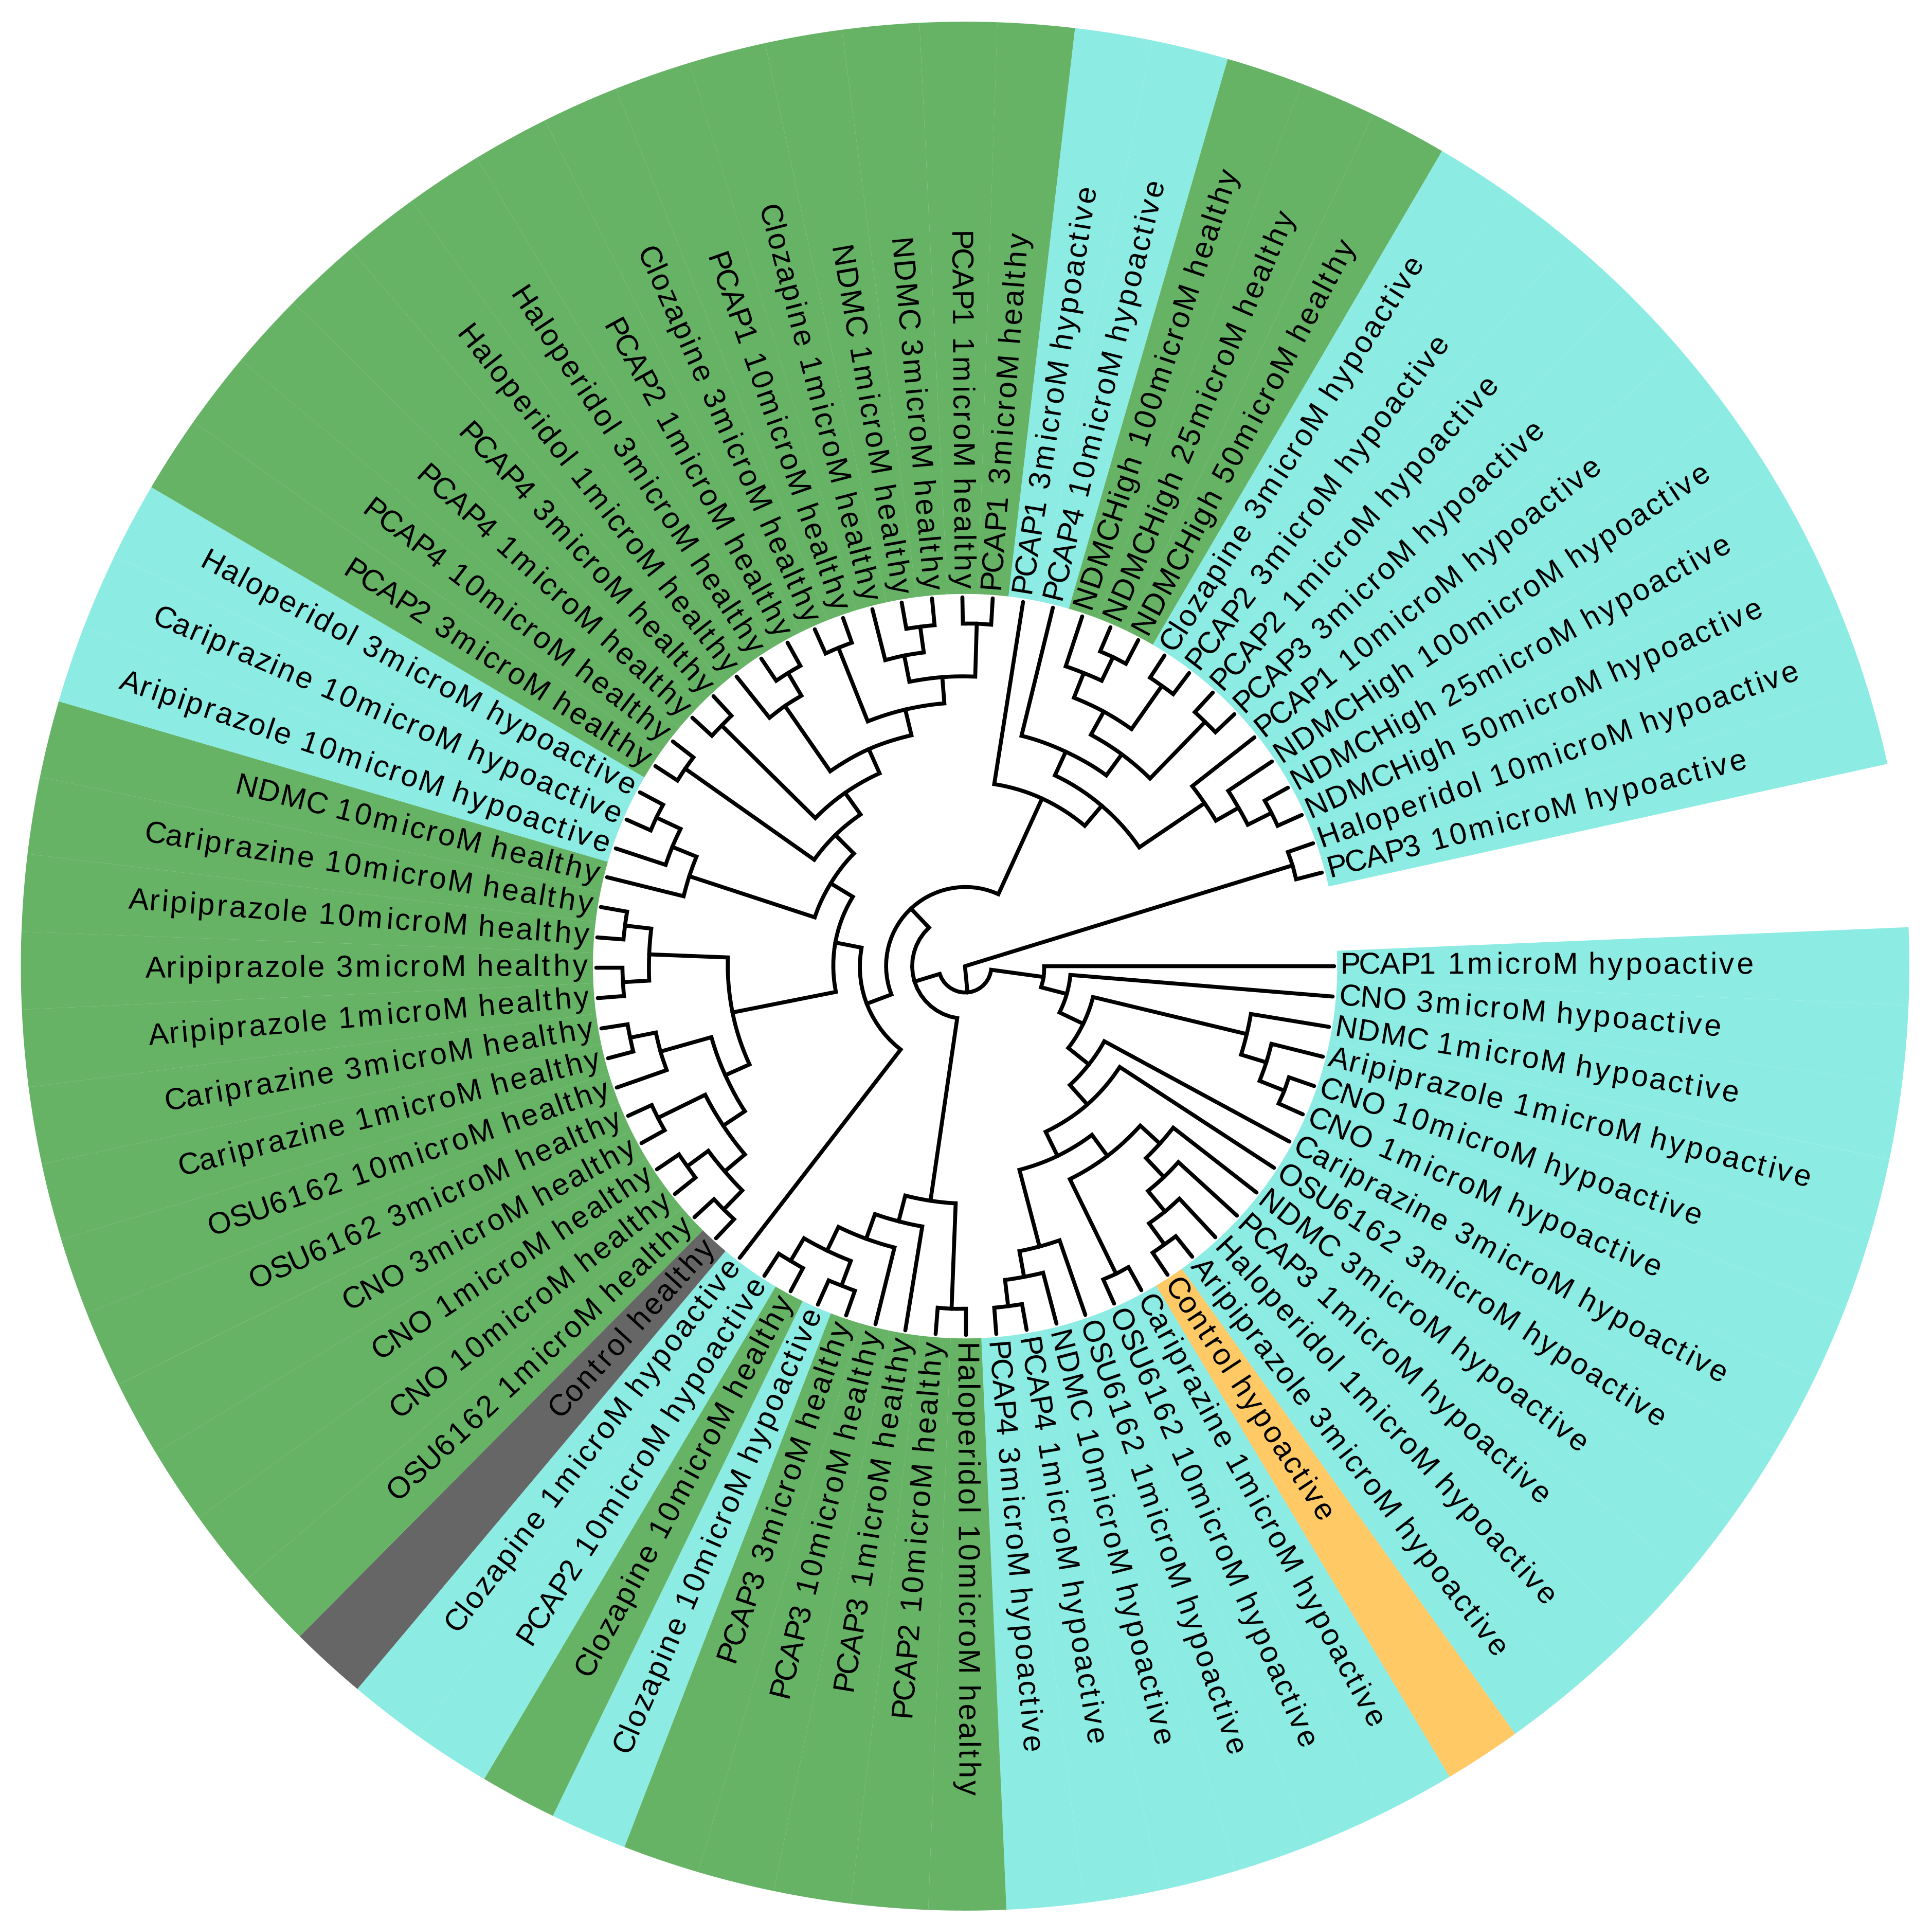
\includegraphics[width=14cm,height=14cm]{DarkApoLow_set1_PCA_tree_A.png}
\caption{Circular cladogram, representing Euclidean distances between the first five principal components of a PCA using the first set of descriptive statistics, for the healthy and hypoactive condition.}
\end{center}
\end{figure}
\newpage
\begin{figure}[h!]
\begin{center}
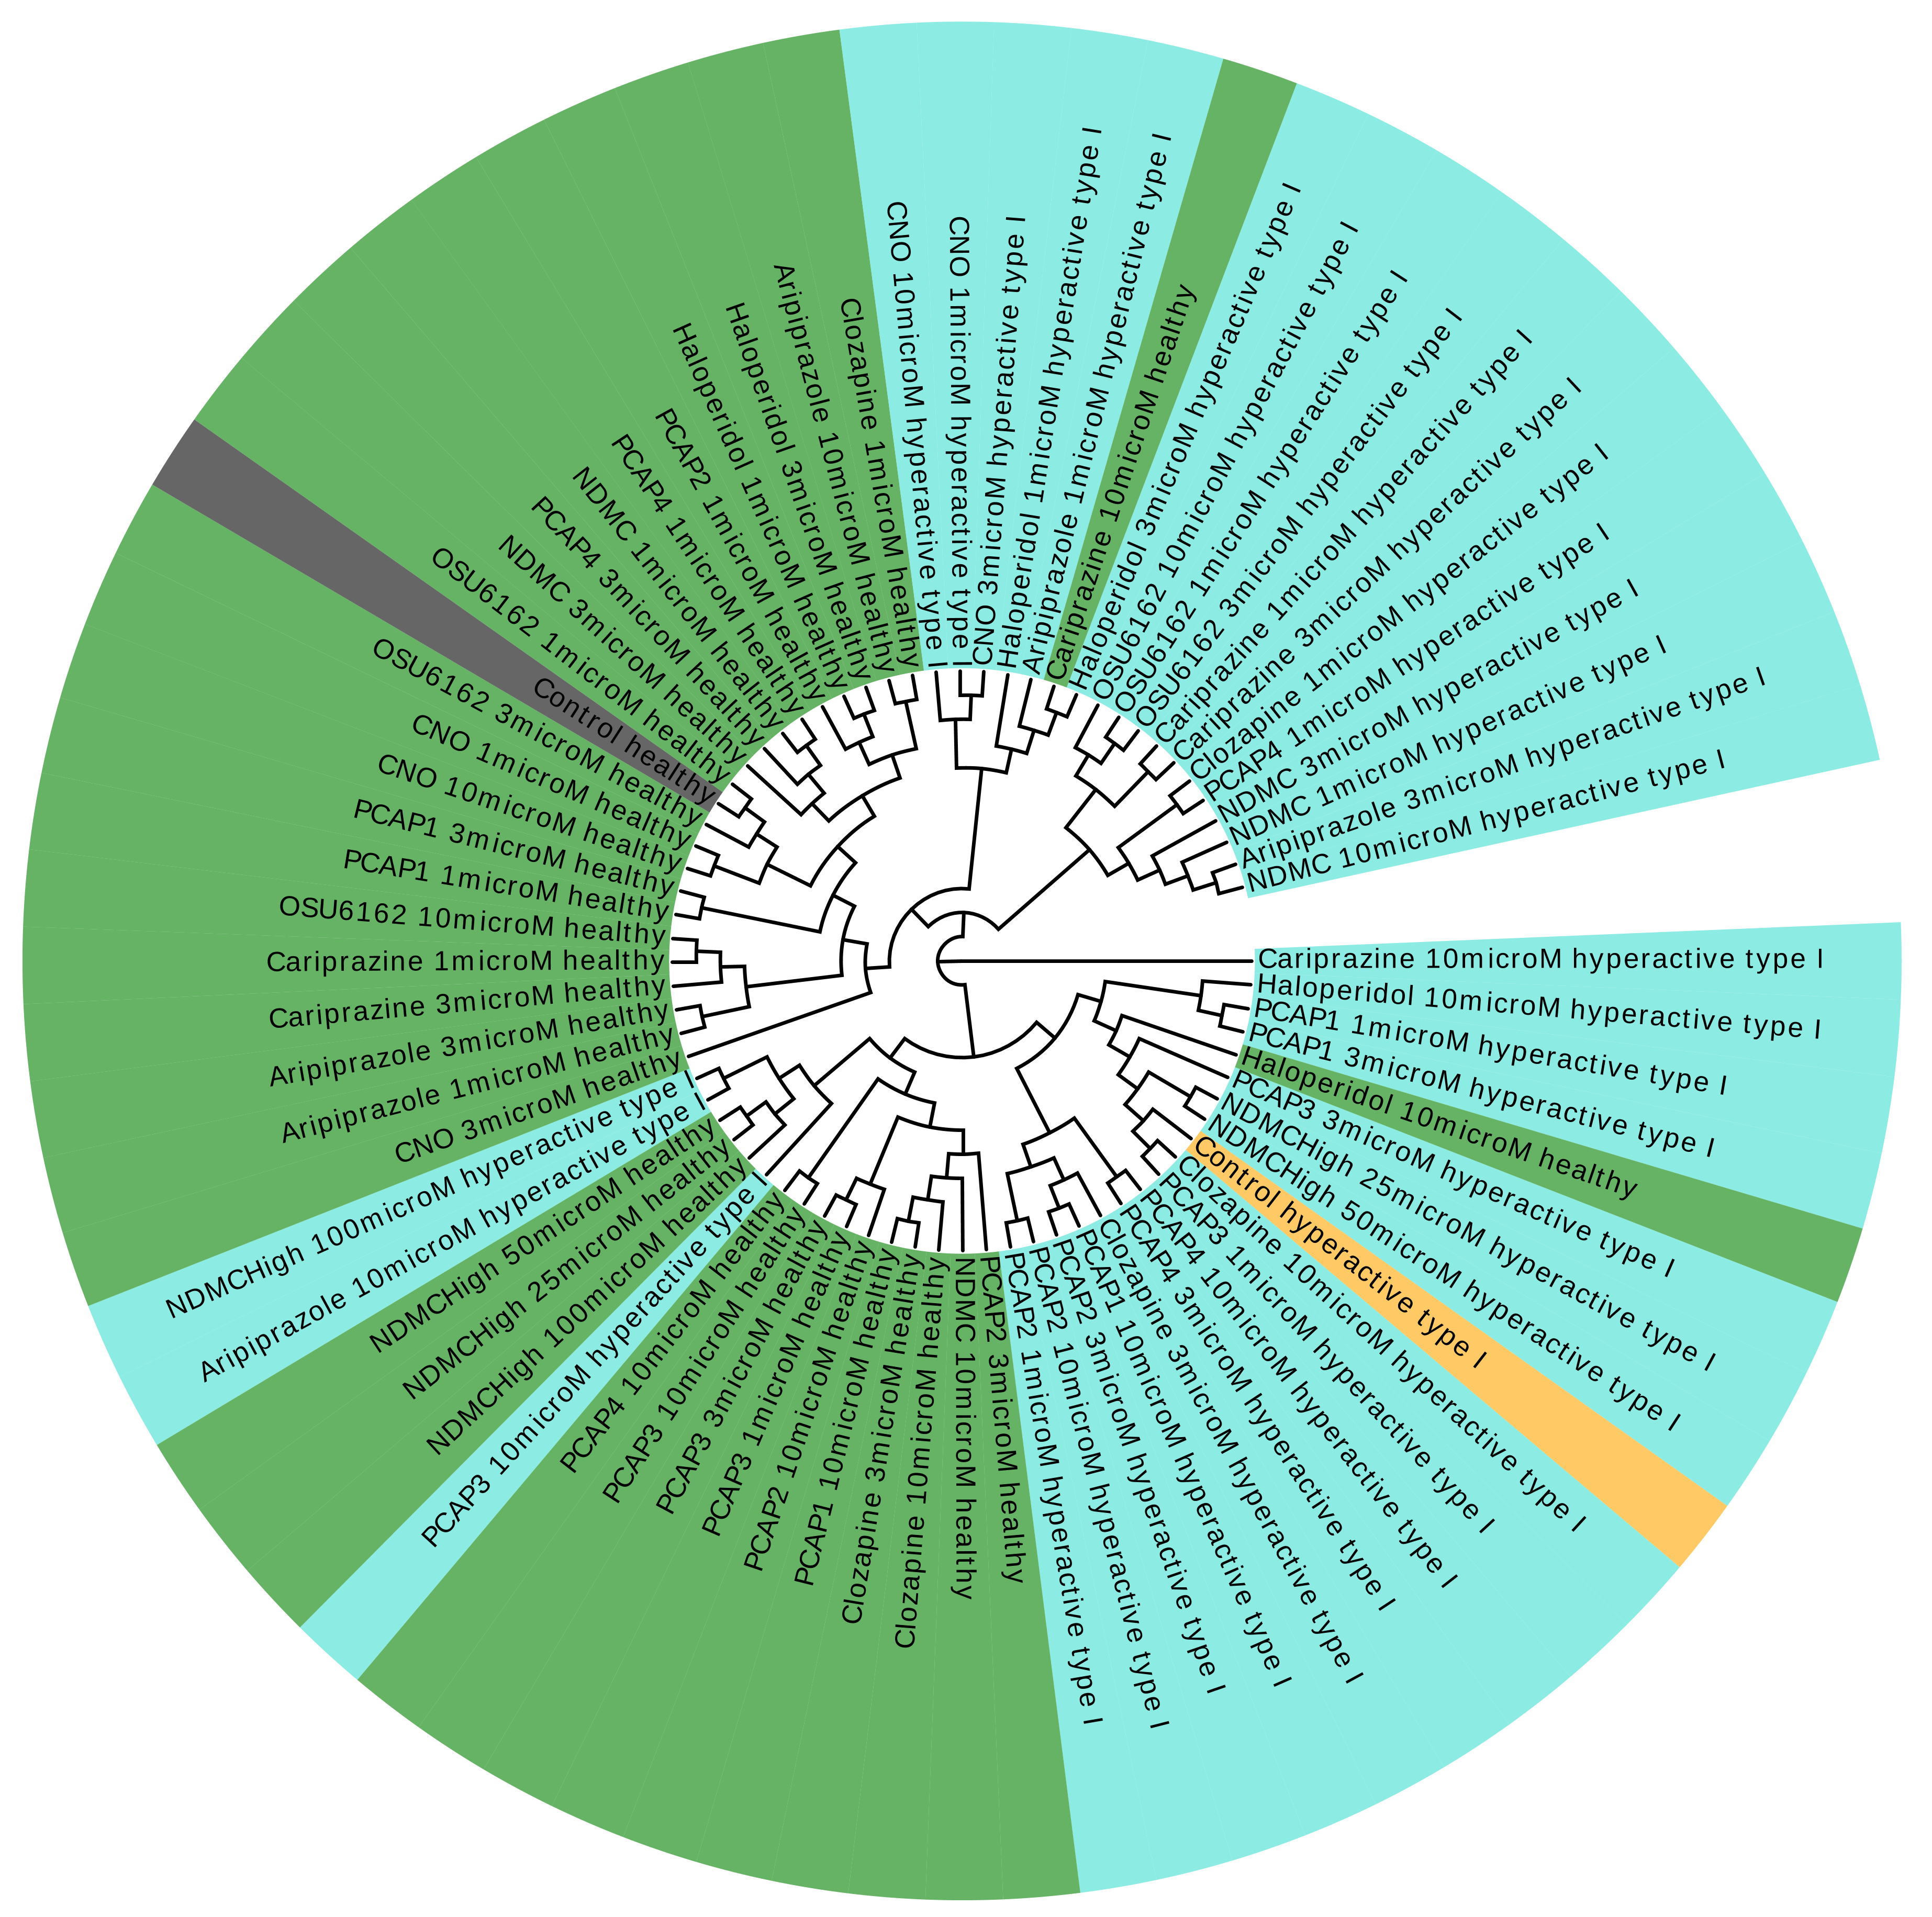
\includegraphics[width=14cm,height=14cm]{DarkApoHigh_set1_PCA_tree_A.png}
\caption{Circular cladogram, representing Euclidean distances between the first five principal components of a PCA using the first set of descriptive statistics, for the healthy and type I hyperactive condition.}
\end{center}
\end{figure}
\newpage
\begin{figure}[h!]
\begin{center}
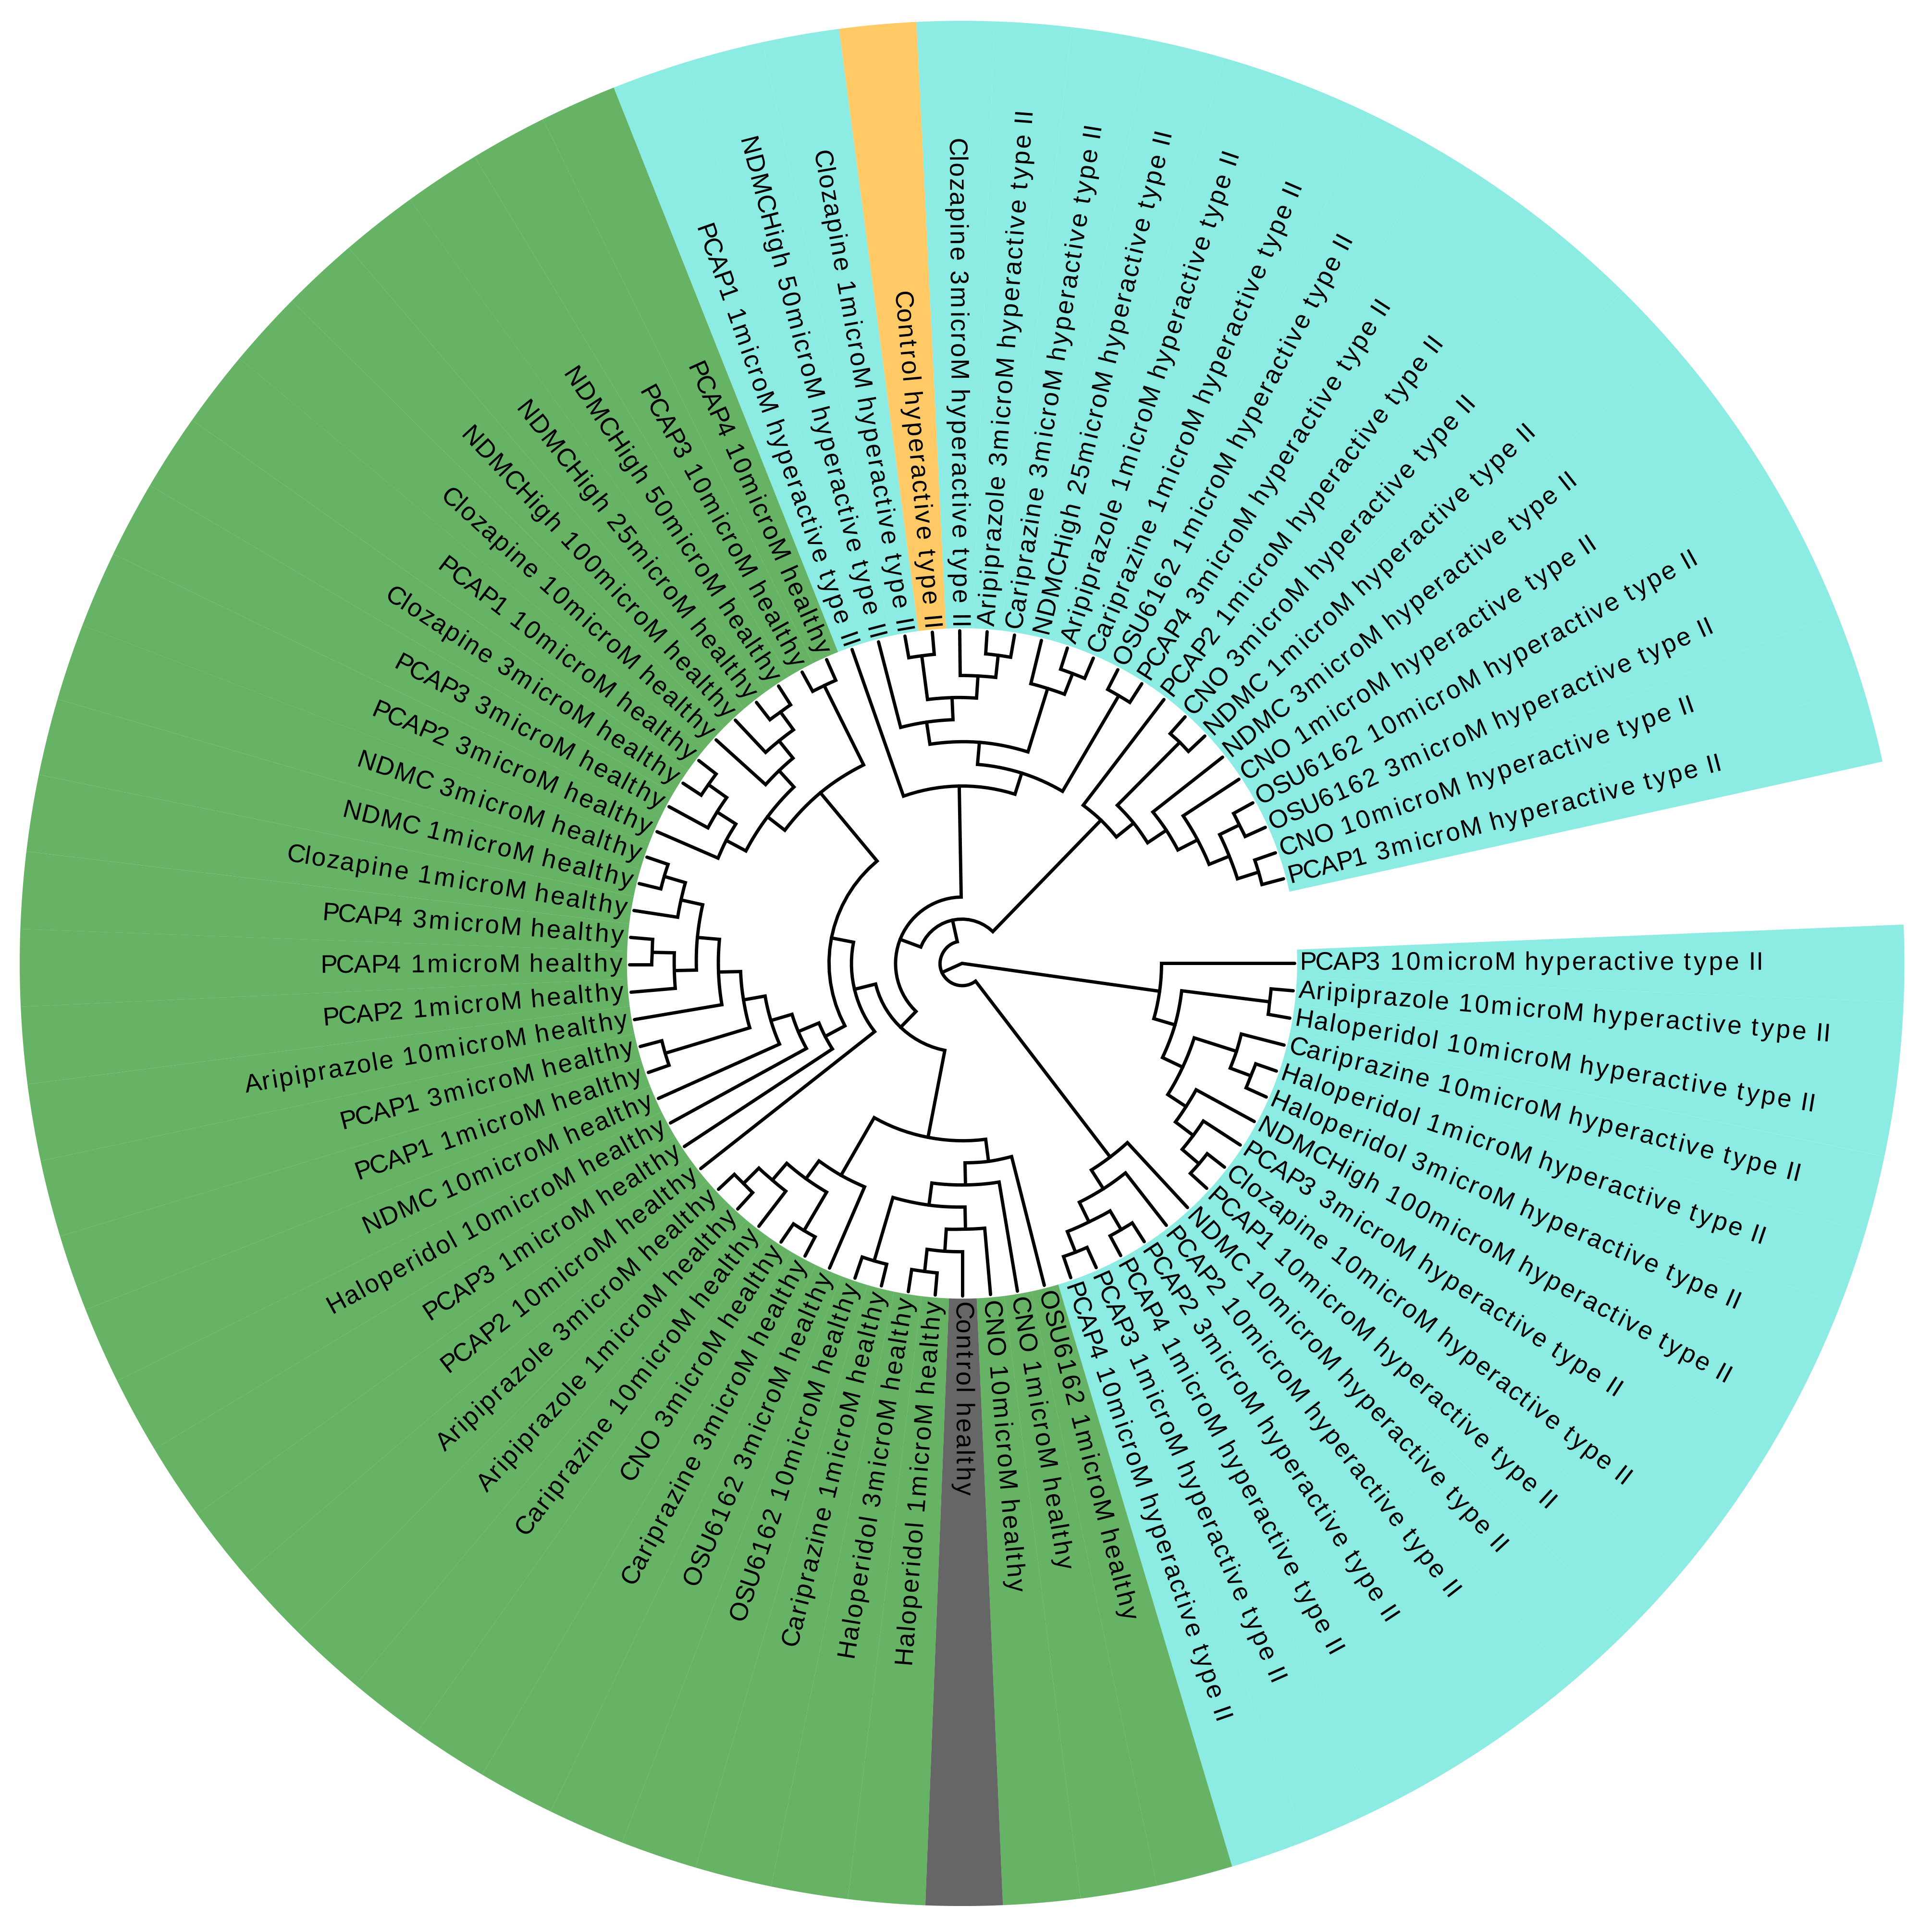
\includegraphics[width=14cm,height=14cm]{DarkPTZ_set1_PCA_tree_A.png}
\caption{Circular cladogram, representing Euclidean distances between the first five principal components of a PCA using the first set of descriptive statistics, for the healthy and type II hyperactive condition.}
\end{center}
\end{figure}
\subsection{Mixed effects analysis}
Results of the mixed effects analyses can provide a more accurate insight into the effects of various compounds on the locomotor phenotypes of the healthy and disease induced larvae when compared to the healthy control. Besides comparing the effects of various compounds, the progression over the time frames can also be analysed and compared, while adjusting for the confounding variables.\\
When comparing the total bout count between the healthy control and the control given a low or a high dose of Apomorphine, effects were as observed in a published study\cite{ref18}, which showed a non-linear response in the total bout count variable. The administration of a low dose of Apomorphine resulted in fewer total bouts, with a slight increase in the first few timeframes, followed with a decrease. The administration of a high dose of Apomorphine resulted in a substantial decrease in the first few timeframes, followed by a substantial increase towards the middle end and a decrease in the end. Table 13 shows the results of the mixed effects analysis for the total bout count variable in the control groups of all three disease induced conditions, multiplicative effects shown with reference to the healthy control group.
\begin{table}[h!]\tiny
\centering
\begin{tabular}{|c|c|c|c|c|}
\hline
%\multirow{2}{}{}                                  & \multicolumn{2}{c|}{assay} & \multicolumn{2}{c|}{progress in time} \\ \cline{2-5}
\multicolumn{5}{|c|}{effects on the total bout count}                              \\ \hline
                                   & \multicolumn{2}{c|}{assay} & \multicolumn{2}{c|}{progress in time} \\ \cline{2-5}
                                   &  $\beta$            & p-value      &      $\beta$              & p-value           \\ \hline
hypoactive condition control group             & 0.163      & \textless2e-16        & 1.078             & 0.083             \\ \hline
type I hyperactive condition control group      & 0.330      & 1.4e-07        & 1.140             & 2.9e-05            \\ \hline
type II hyperactive condition control group    & 0.332     & 3.1e-06        & 1.088             & 0.019             \\ \hline
\end{tabular}
\caption{Multiplicative effect on the total bount count when compared to the healthy control group.}
\end{table}

\\Published analyses of bout count, bout distance and turn proportions\cite{ref18} were extended in this project and analysed with more precision, focusing on the additional compounds being administrated along with each of the disease inducing compounds and their effects on the turn and turn transition variables.
\\Heatmaps were constructed and plotted based on the effect sizes of the first 25 variables with the biggest absolute multiplicative effect size, for each of the three disease induced conditions and the first and third set of descriptive statistics, all figures shown in Appendix D.1 and D.2.\\Figures 18, 19 and 20 show examples of heatmaps of the effect sizes for the overall group difference in the hypoactive, type I hyperactive and the type II hyperactive condition, respectively. The heatmaps in Figures 18, 19 and 20 were constructed using the first set of descriptive statistics, where variable importance and compound ranking can be seen in the grouping/order of the rows and columns, respectively. Dendrogram branches had to be excluded from the plots, as they did not fit the width of the page.
\newpage
\begin{figure}[h!]
\begin{center}
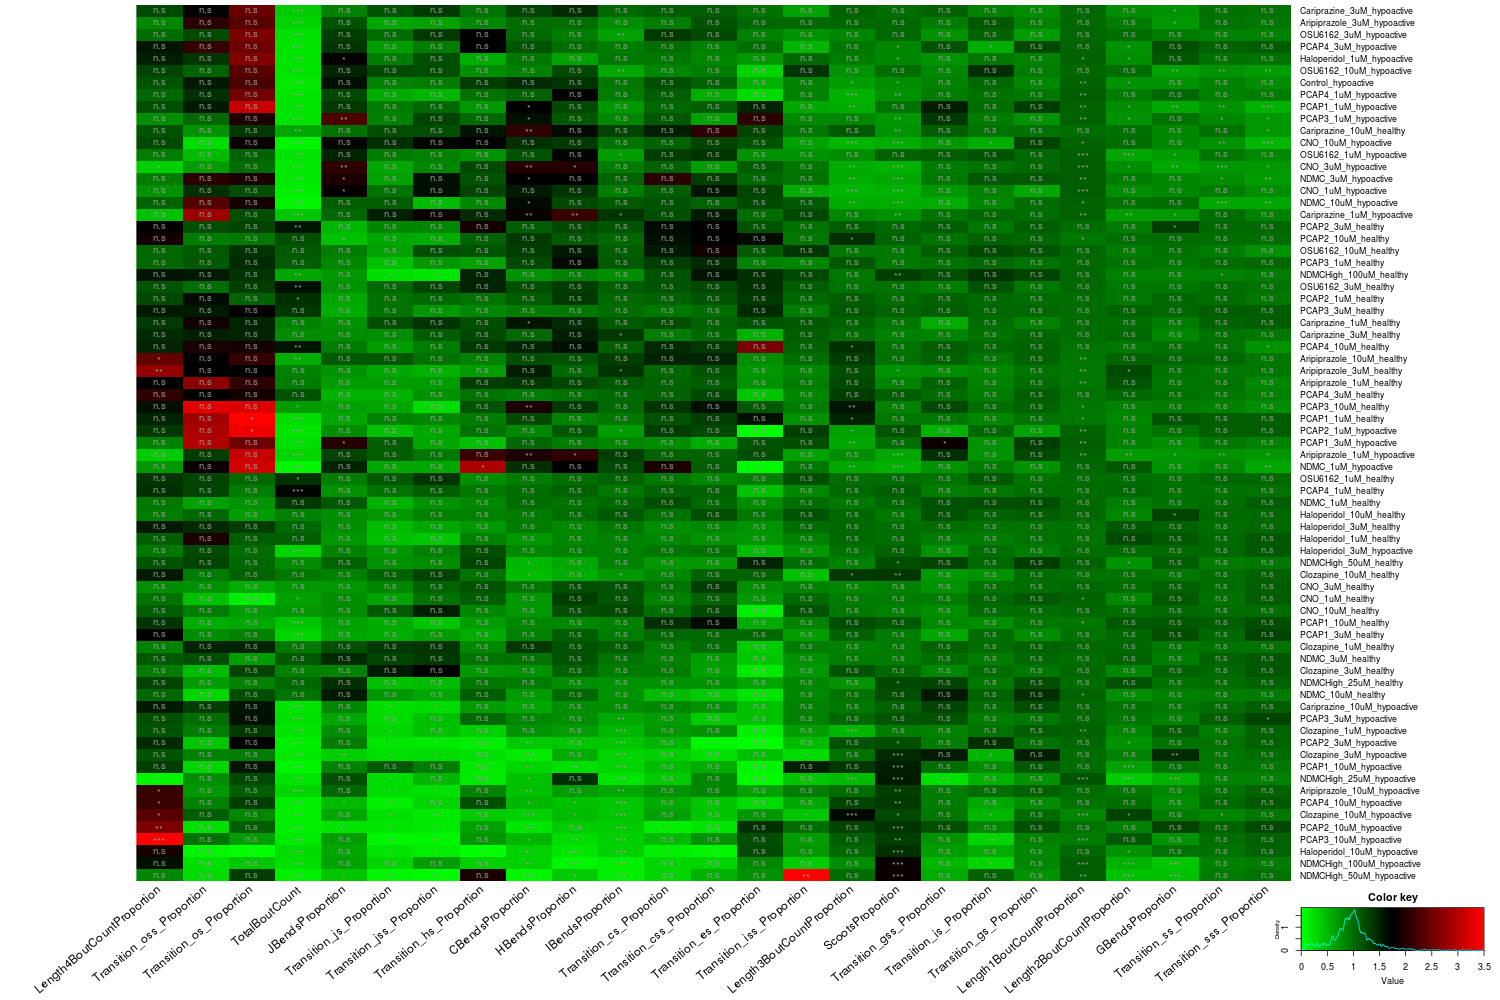
\includegraphics[width=16cm,height=15cm]{DarkApoLow_heatmap_all_DarkApoLow_B2MAP.png}
\caption{Heatmap, for the hypoactive condition, using the first set of descriptive statistics, showing the multiplicative effect sizes colour coded and noted with the significance level.}
\end{center}
\end{figure}
\newpage
\begin{figure}[h!]
\begin{center}
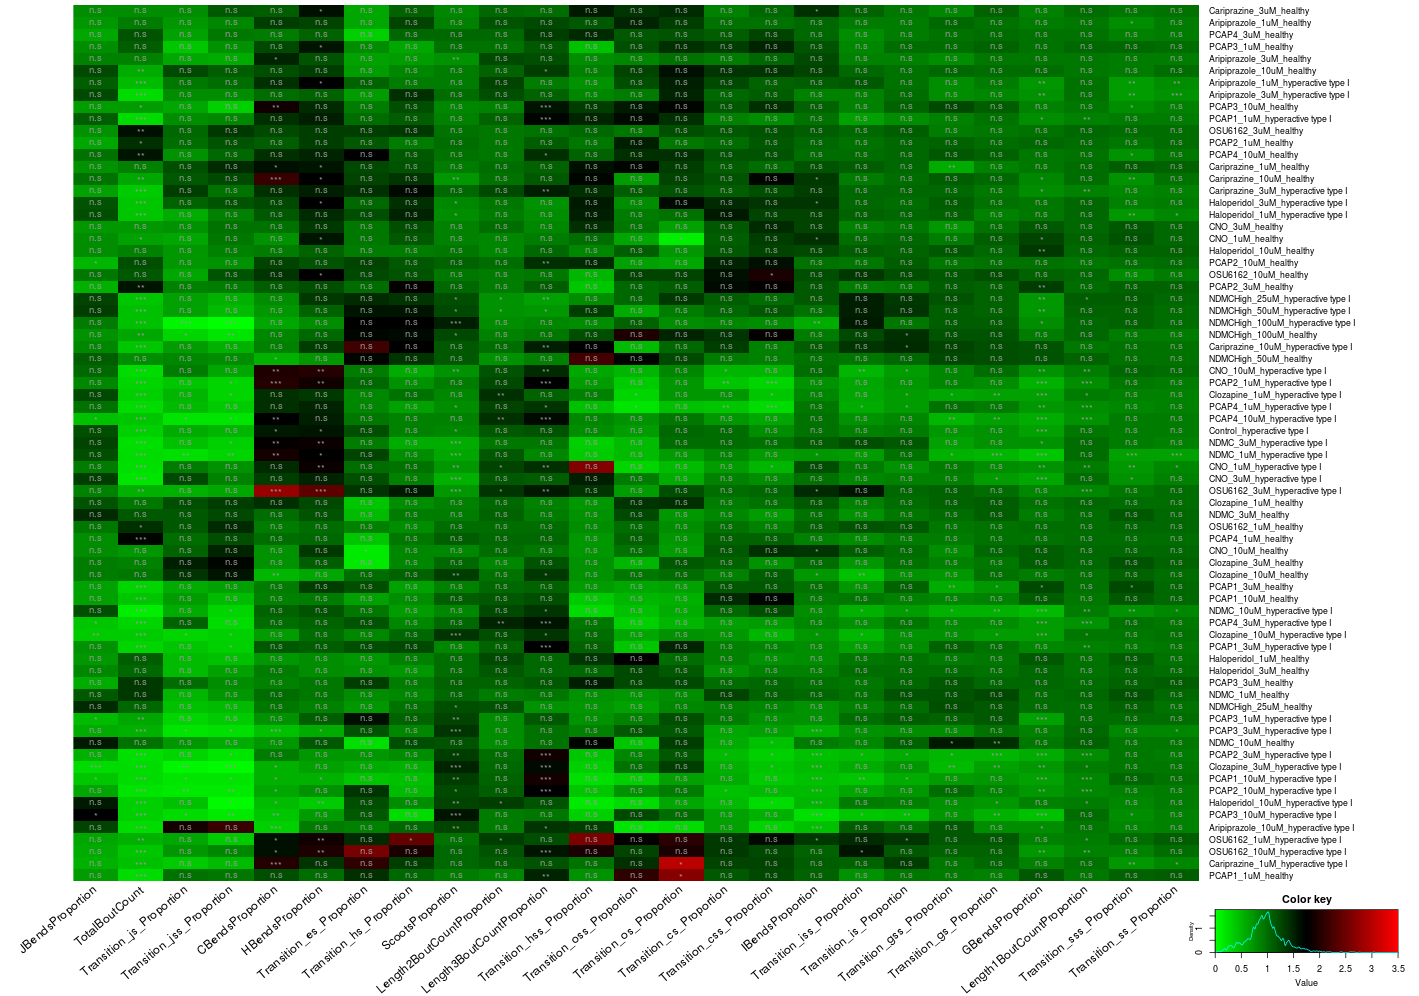
\includegraphics[width=16cm,height=15cm]{DarkApoHigh_heatmap_all_DarkApoHigh_B2MAP.png}
\caption{Heatmap, for the type I hyperactive condition, using the first set of descriptive statistics, showing the multiplicative effect sizes colour coded and noted with the significance level.}
\end{center}
\end{figure}
\newpage
\begin{figure}[h!]
\begin{center}
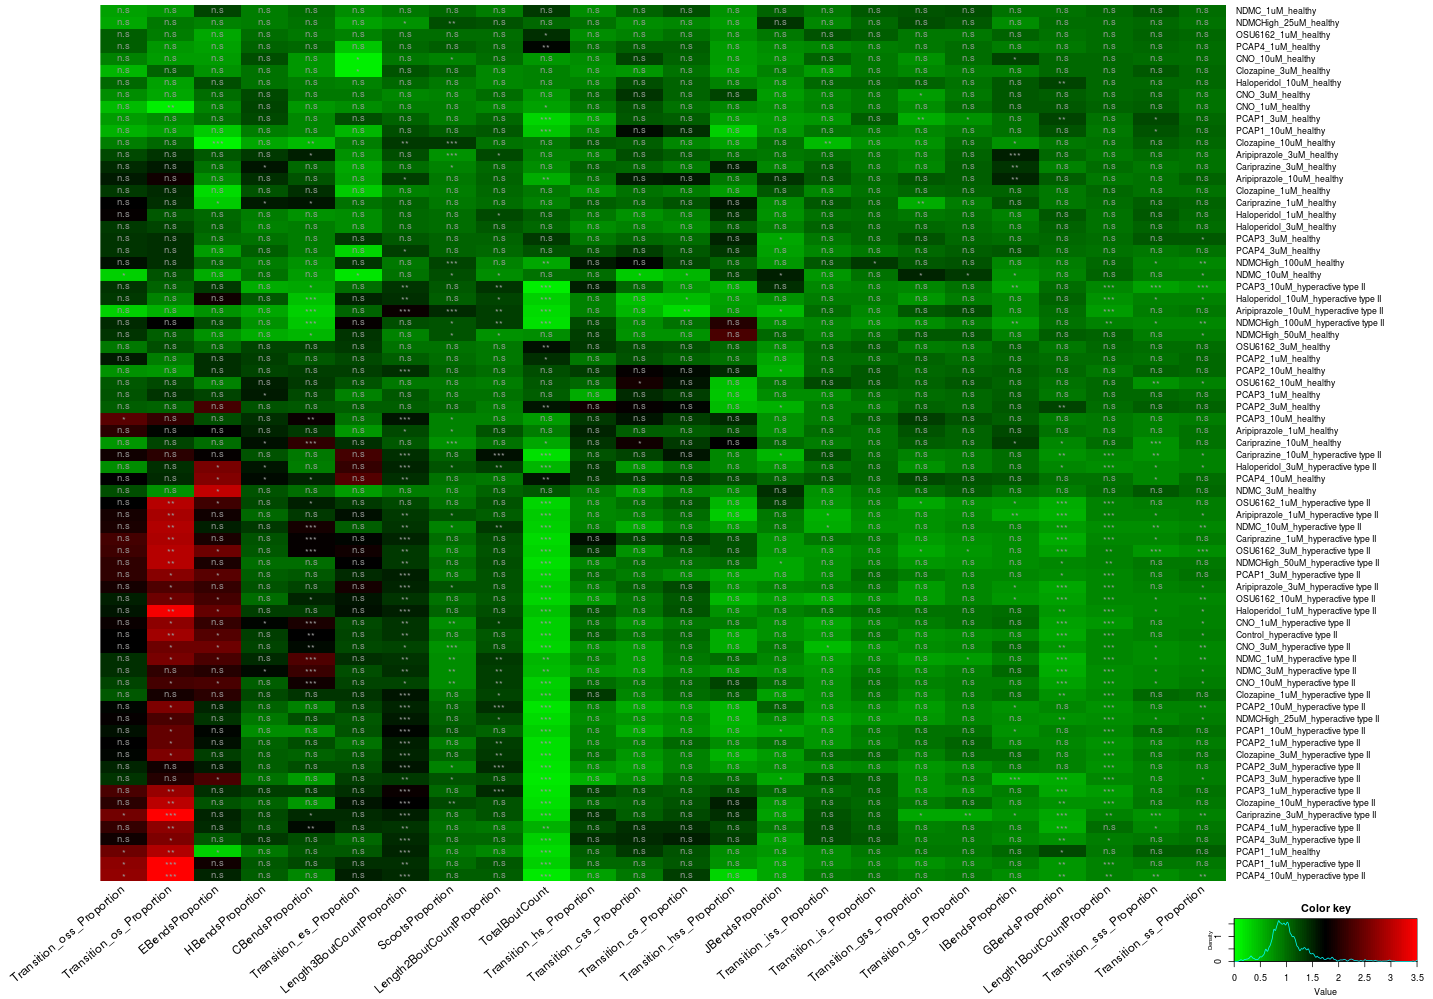
\includegraphics[width=16cm,height=15cm]{DarkPTZ_heatmap_all_DarkPTZ_B2MAP.png}
\caption{Heatmap, for the type II hyperactive condition, using the first set of descriptive statistics, showing the multiplicative effect sizes colour coded and noted with the significance level.}
\end{center}
\end{figure}
\newpage
\section{Closure}
\subsection{Discussion}
The aim of the current project was to analyse zebrafish larvae action sequences, in order to compare and profile several different drugs for therapeutic purposes in neurological diseases.\\The information contained in the action sequences had to be linked to the larval neurological state and therefore required extraction into descriptive statistics representing larval locomotor phenotypes. Certain patterns or abnormalities in the action sequences have already been linked to the larval neurological state, ranging from simple and general locomotor phenotypes like total count of swim bouts and duration/length of swim bouts to more detailed locomotor phenotypes like the total proportion of certain turn types, while lacking precision and advanced locomotor phenotypes, which would represent turn transitions or turn patterns.
\\The larvae action sequence recording and construction techniques, which produced the action sequence data in this project, are novel and state of the art approaches, which enabled accurate measurement of larval movement to the extent of a single turn and therefore accurate measurement of larval neurological behaviour in a vast collection of compound screening assays. With such a high throughput of detailed measurements, the data analysis and interpretation of results can become complicated and error-prone.
\\The action sequences in this project consisted of sequences of letters, representing turn types, organized in swim bouts. Changes in the overall turn type proportions were subjected to confounding by the overall bout count and bout length, while the changes in the turn transitions or turn patterns were additionally subjected to confounding by the turn proportion variables.\\For example, the overall proportion of \textit{Scoots} was very high in longer bouts, while in shorter bouts, particularly bouts of length one, the overall turn proportions were less biased. Such confounding could result in a significant change in turn proportions, due to a change in bout length only. Therefore, if a compound reduces the length of the larval swim bouts, it could consequentially result in a smaller overall proportion of \textit{Scoots} and a larger overall proportion of other turn types, including \textit{C-bends} or \textit{O-bends}, which would be in this case misleading. A true significant change in the overall proportion of \textit{C-bends} or \textit{O-bends}, when comparing to the healthy control group, could indicate that the compound has stress-like behaviour inducing properties, resulting in the larvae performing more escape turns, but if the change actually only reflects the reduced bout length and the true turn proportions are not changed, the larvae could actually not be stressed, but sedated only. Such confounding had to be taken into account when performing data analysis and interpretation of results. 
\\Locomotor phenotypes were represented by descriptive statistics in the form of count data. Due to a large amount of information, a complicated experimental design and simplicity of the current project, the locomotor phenotypes were being modelled per action sequence and not per swim bout. This meant that count data was extracted from different assays and time frames within the assay, resulting in different degrees of variance stability and therefore additional confounding by the bout count, which also had to be taken into account.\\Large amount of information coming from a complicated experimental design, count data variables with a high variation in within and between assay variance and the presence of confounding were considered in this project, while aiming to compare and profile several different drugs with a focus on turn proportions and turn transition proportions.
\\Several different data sets of descriptive statistics were used to perform exploratory data analysis, in order to observe the general trends in the data, as well as influences of confounding. Confounding was confirmed with simple correlation or partial correlation tests and was not explored in a separate analysis, something that is left to be done in the future, when designing and implementing a more detailed analysis on the bout level, or even on a single turn level.\\Exploratory data analysis of different data sets was performed with a PCA and revealed strong trends showing changes between the assays, as well as in the progress through the time frames. These trends were visually very similar between the two data sets of descriptive statistics, where turn and turn transition proportions were not stratified in bout length, one including and the other not including bout count and bout length variables, with the exception of the hypoactive condition, where substantial changes were visible. This could mean that most of the variation comes from the turn and turn transition proportion variables, or it could mean that the proportion of variation in the turn and turn transition variables, attributable to bout count and bout length changes, is substantial enough to result in so similar principal components, where a Pearson's correlation test between the first principal components resulted in R=0.98, with a p-value \textless2e-16.
\\Variable influence was estimated based on correlation tests between the variables and the first five principal components and differed substantially between the three different disease induced conditions. Most of the highly influential variables in the hypoactive condition were turn and turn transition variables, less so in the type I hyperactive condition and in the type II hyperactive condition, where the number of influential turn and turn transition variables was more or less the same as the number of influential bout count and bout lenght variables.
\\Although this does not make the results of compound ranking and grouping incorrect, there is a possibility that the trends do not reflect the variation in turn and turn transition variables attributable to influences of compounds and time frames directly and independently of bout count and bout length variables, which is the focus of the analysis in the current project.
\\Two additional sets of descriptive statistics were extracted and used to conduct PCA. In both additional sets, turn and turn transition variables were extracted per bout length stratum, in order to avoid influences of the variation in bout length. Stratification in bout length consequently increased the number of variables approximately threefold. In the first additional set bout count and bout length variables were included and in the second set, these variables were excluded from the PCA. The results visually differed from the results obtained with the first two sets, but were nevertheless similar between each other as in the previous case. Even though the majority of the estimated influential variables in the third set of descriptive statistics were turn and turn transition variables, which have been extracted per bout length stratum, there was still a possibility that the overall variation being projected on the first principal component contains variation sourcing from the bout count variables, since variance stability differed between the count data of different assays and time frames within the assay.\\Appart from the uncertainty regarding the source of variation in the turn and turn transition variables, the PCA results provided interesting information and showed a lot of trends, which could be explained from the point of view of neurological diseases and their medication. Several possible outcomes could be explored by examining the proximity of compound clusters to the clusters of the healthy control and the disease induced control:
\begin{itemize}
  \item \textit{Close to the healthy control cluster and close to the disease induced cluster}, resulting from compounds with no effect on the healthy or disease induced controls,
  \item \textit{Close to the healthy control cluster but far from the disease induced cluster, going in direction away from the healthy control}, resulting from compounds with no unwanted effects on the healthy control, while having unwanted effects on the disease induced control,
  \item \textit{Close to the healthy control cluster but far from the disease induced cluster, going in direction towards the healthy control}, resulting from optimal compounds which have no unwanted effects on the healthy control and wanted effects on the disease induced control,
  \item \textit{Far from the healthy control cluster and far from the disease induced cluster, going in direction towards the healthy control}, resulting from compounds with unwanted effects on the healthy control, while having wanted effects on the disease induced control,  
  \item \textit{Far from the healthy control cluster and far from the disease induced cluster, going in direction away from the healthy control}, resulting from compounds with unwanted effects on the healthy control and on the disease induced control,    
  \item \textit{Far from the healthy control cluster and close to the disease induced cluster}, resulting from compounds with unwanted effects on the healthy control and no effects on the disease induced control.
\end{itemize}
\\
These outcomes were summarized to show vectors representing direction in the change through time or in the change through dosage, which enabled direct comparison of compound effects in time and in dosage.
\\Generalized linear mixed model analyses were performed to further adjust for the confounding variables and obtain the direct and independent compound effects on the turn and turn transition variables. Variable influence and compound ranking could be seen in the heatmaps of the multiplicative effect sizes with reference to the control. Besides the total bout count, the influential variables were turn and turn transition variables.\\Although there were significant changes in the turn transition variables, the transitions mainly included routine turn types or normal escape patterns. No changes could be detected in the distinct turn transition or turn patterns, that could be linked to the abnormal neurological state of the larvae, like for example abnormal execution of an escape turn. When examining the first 30 highest proportions of turn transitions per entire control group through all time frames combined, only the type II hyperactive condition control group contained transitions with two or even three consecutive \textit{C-bends}, which can be considered a sign of an abnormal neurological state. Reasons to why changes in the counts of these transitions could not be confirmed with the statistical analyses could be that these changes in counts are merely due to the change in bout length and bout count or could be that there was too few of these transitions considering the total amount of words of length two or three. These reasons could also apply to the substantial amount of non-significant effects of certain compounds, particularly when observing the effect in time.\\Besides improving the analyses to appropriately account for confounding and variance stability, improvements are also needed to better represent the results and enable a user-friendly exploration. Compound screening technologies based on zebrafish larvae action sequences can produce a vast amount of information, usually for more than 12 compounds. Results from analyses should be as summarized as possible with clear notations and accesible through a graphical interface.
\subsection{Conclusions}
Conclusions from the zebrafish larvae action sequence analysis:
\begin{itemize}
  \item Zebrafish larvae locomotor phenotypes, extracted from action sequences, are likely to be non-normally distributed, heteroscedastic count variables,
  \item The length and frequency of swim bouts will influence the overall proportion of turns and turn transitions, 
  \item Turn transitions are additionally influenced by the turn proportions,
  \item Exploratory data analysis like PCA will show trends of overall compound effects and compound effects through time and dosage, 
  \item PCA results are susceptible to reflect confounding by bout count and bout length, therefore not providing reliable estimates regarding turn and turn transition variables, 
  \item Stratification in bout length can improve the results, but will drastically increase the number of variables and make interpretation of results less clear,
  \item General linear mixed models can estimate the direct compound effect on the turn and turn transition variables,
  \item Compound effects were ranked and grouped, as well as represented to show direction of changes through time and dosage, therefore enabling linkage to the larval neurological state,
  \item The count of certain turn transitions could have been too low to detect significant trends in this project.
\end{itemize}
\newpage
%%%%%%%%%%%%%%%%%%%%%%%%%%%%%%%%%%%%%%%%%%%%%%%%%%%%%%%%%%%%%%%%%%%%%%%%%%
\begin{thebibliography}{99}
\bibitem{ref1}
Brittijn S.A., Duivesteijn S.J., Belmamoune M., Bertens L.F.M., Bitter W., de Bruijn J.D., Champagne D.L., Cuppen E., Flik G., Vandenbroucke-Grauls C.M., et al. Zebrafish development and regeneration: New tools for biomedical research. \textit{Int. J. Dev. Biol.} \textbf{53} 835-850 (2009).
\bibitem{ref2}
Zon L.I., Peterson R.T. In vivo drug discovery in the zebrafish. \textit{Nature Reviews Drug Discovery.} \textbf{4} 35-44 (2005).
\bibitem{ref3}
Grunwald D.J., Eisen J.S. Headwaters of the zebrafish-Emergence of a new model vertebrate. \textit{Nat. Rev. Genet.} \textbf{3} 711-724 (2002).
\bibitem{ref4}
Barros, T. P., Alderton, W. K., Reynolds, H. M., Roach, A. G. \& Berghmans, S. Zebrafish: an emerging technology for 
in vivo pharmacological assessment to identify potential safety liabilities in early drug discovery. \textit{Br. J. Pharmacol.}
\textbf{154}: 1400-13 (2008).
\bibitem{ref5} 
Oliveira R. F. Mind the fish: zebrafish as a model in cognitive social neuroscience. \textit{Front. Neural Circuits} \textbf{7} 131 (2013).
\bibitem{ref6} 
Best J. D., and Alderton W. K. Zebrafish: an in vivo model for the study of neurological diseases. \textit{Neuropsychiatr. Dis. Treat.}
\textbf{4} 567-576 (2008).
\bibitem{ref7} 
Stewart A.M., Braubach O., Spitsbergen J., Gerlai R., Kalueff A.V. Zebrafish models for translational neuroscience research: from tank to bedside. \textit{Trends in neurosciences.} \textbf{37} 264-278(2014).
\bibitem{ref8} 
Orger M.B., Gahtan E., Muto A., Page-McCaw P., Smear M.C., Baier H. Behavioral screening assays in zebrafish. \textit{Methods Cell Biol.} \textbf{77} 53-68(2004).
\bibitem{ref9} 
Budick S.A., O’Malley D.M. Locomotor repertoire of the larval zebrafish: swimming, turning and prey capture. \textit{J Exp Biol.} \textbf{203} 2565-79 (2000).
\bibitem{ref10} 
Anichtchik O.V., Kaslin J., Peitsaro N., Scheinin M., Panula P. Neurochemical and behavioural changes in zebrafish Danio rerio after systemic administration of 6-hydroxydopamine and 1-methyl-4-phenyl-1,2,3,6-tetrahydropyridine. \textit{J. Neurochem.} \textbf{88} 443-453 (2004). 
\bibitem{ref11} 
Pfeiffer R.F., Gutmann L., Hull K.L. Jr, Bottini P.B., Sherry J.H., Investigators APOS. Continued efficacy and safety of subcutaneous apomorphine in patients with advanced Parkinson's disease. \textit{Parkinsonism Relat Disord} \textbf{13} 93-100 (2007).
\bibitem{ref12} 
Tamminga C.A., Schaffer M.H., Smith R.C., Davis J.M. Schizophrenic symptoms improve with apomorphine. \textit{Science.} \textbf{200} 567-568 (1978).
\bibitem{ref13} 
Ljungberg T., Ungerstedt U. Classification of neuroleptic drugs according to their ability to inhibit apomorphine-induced locomotion and gnawing: Evidence for two different mechanisms of action. \textit{Psychopharmacology (Berl)} \textbf{56} 239-247 (1978). 
\bibitem{ref14} 
Ellis L.D., Seibert J., Soanes K.H. Distinct models of induced hyperactivity in zebrafish larvae. \textit{Brain Res} \textbf{1449} 46-59 (2012). 
\bibitem{ref15}
Ellis L.D., Soanes K.H. A larval zebrafish model of bipolar disorder as a screening platform for neuro-therapeutics. \textit{Behav Brain Res.} \textbf{233} 450-457 (2012).
\bibitem{ref16}
Serra E.L., Medalha C.C., Mattioli R. Natural preference of zebrafish (Danio rerio) for a dark environment. \textit{Braz J Med Biol Res.} \textbf{32(12)} 1551-1553(1999). 
\bibitem{ref17} 
Ek F., et al. Behavioral Analysis of Dopaminergic Activation in Zebrafish and Rats Reveals Similar Phenotypes. \textit{ACS Chem. Neurosci.} \textbf{7} 633-46 2016.
\bibitem{ref18} 
Palmer T., Ek F., Enqvist O., Olsson R., Åström K., Petersson P. Action sequencing in the spontaneous swimming behavior of zebrafish larvae - implications for drug development. \textit{Sci Rep.} \textbf{7} 3191(2017). 
\bibitem{ref19} 
Korn H., Faber D.S. The Mauthner cell half a century later: a neurobiological model for decision-making? \textit{Neuron.} \textbf{47} 13-28 (2005).
\bibitem{ref20} 
Lorent K., Liu K.S., Fetcho J.R., Granato M. The zebrafish space cadet gene controls axonal pathfinding of neurons that modulate fast turning movements. \textit{Development.} \textbf{128} 2131-2142 (2001).
\bibitem{ref21} 
Bhandiwad A. A., Zeddies D. G., Raible D. W., Rubel E. W., Sisneros J. A. Auditory sensitivity of larval zebrafish (Danio rerio) measured using a behavioral prepulse inhibition assay. \textit{Journal of Experimental Biology.} \textbf{216(18)} 3504-3513 (2013).
\bibitem{ref22}
Tanji J. Sequential organization of multiple movement: involvement of cortical motor areas. \textit{Annu. Rev. Neurosci.} \textbf{24} 631-651 (2001).
\bibitem{ref23}
Kasparek T., Rehulova J., Kerkovsky M., Sprlakova A., Mechl M., Mikl M. Cortico-cerebellar functional connectivity and sequencing of movements in schizophrenia. \textit{BMC Psychiatry} \textbf{12} 17 (2012).
\bibitem{ref24}
Caligiore D., Helmich R.C., Hallett M., Moustafa A.A., Timmermann L., Toni I., Baldassarre G. Parkinson's disease as a system-level disorder. \textit{Npj Park. Dis.} \textbf{2} 16025 (2016).
\bibitem{ref25} 
Liu Y., Ma P., Cassidy P.A., Carmer R., Zhang G., Venkatraman P., Brown S.A., Pang C.P., Zhong W., Zhang M., Leung Y.F. Statistical Analysis of Zebrafish Locomotor Behaviour by Generalized Linear Mixed Models. \textit{Scientific Reports.} \textbf{7} 2937 (2017).
\bibitem{ref26} 
Liu, Y. et al. Statistical analysis of zebrafish locomotor response. \textit{PLoS One} \textbf{10} (2015).

\bibitem{ref27}
Wikipedia, The Free Encyclopedia, s.v.  "Aripiprazole" (accessed July 11, 2017) https://en.wikipedia.org/wiki/Aripiprazole
\bibitem{ref28} 
Wikipedia, The Free Encyclopedia, s.v.  "Cariprazine" (accessed July 11, 2017) https://en.wikipedia.org/wiki/Cariprazine
\bibitem{ref29} 
Wikipedia, The Free Encyclopedia, s.v.  "Clozapine" (accessed July 11, 2017) https://en.wikipedia.org/wiki/Clozapine
\bibitem{ref30} 
MacLaren D.A., Browne R.W., Shaw J.K., Radhakrishnan S.K., Khare P., Espana R.A., Clark S.D. Clozapine-n-oxide administration produces behavioral effects in Long-Evans rats - implications for designing DREADD experiments. \textit{eneuro} \textbf{3} 5 (2016).
\bibitem{ref31}
Wikipedia, The Free Encyclopedia, s.v.  "Haloperidol" (accessed July 11, 2017) https://en.wikipedia.org/wiki/Haloperidol
\bibitem{ref32}  
Wikipedia, The Free Encyclopedia, s.v.  "Desmethylclozapine" (accessed July 11, 2017) https://en.wikipedia.org/wiki/Desmethylclozapine
\bibitem{ref33}  
Wikipedia, The Free Encyclopedia, s.v.  "OSU-6162" (accessed July 11, 2017) https://en.wikipedia.org/wiki/OSU-6162
\bibitem{ref34}  
Lameh J., McFarland K., Ohlsson J., Ek F., Piu F., Burstein E., et al. Discovery of potential antipsychotic agents possessing pro-cognitive properties. \textit{Naunyn Schmiedebergs Arch Pharmacol} \textbf{385} 313-2310 (2012).
\bibitem{ref35}  
Chawla N.V., Bowyer K.W., Hall L.O., Kegelmeyer P.W. SMOTE: Synthetic Minority Over-sampling Technique. \textit{Journal of Artificial Intelligence Research} \textbf{16} 321-357 (2002).
\bibitem{ref36}  
Wikipedia, The Free Encyclopedia, s.v.  "Random forest" (accessed July 11, 2017) https://en.wikipedia.org/wiki/Random forest
\bibitem{ref37}  
Wikipedia, The Free Encyclopedia, s.v.  "Principal component analysis" (accessed July 11, 2017) https://en.wikipedia.org/wiki/Principal component analysis
\bibitem{ref38}  
Le, S., Josse, J., Husson, F. FactoMineR: An R Package for Multivariate Analysis. \textit{Journal of Statistical Software.} \textbf{25(1)} 1-18 (2008).
\bibitem{ref39}  
Zhang et al. EvolView, an online tool for visualizing, annotating and managing phylogenetic trees. \textit{Nucleic Acids Res} \textbf{4} (2012).
\bibitem{ref40}
Package 'gplots' (accessed July 11, 2017) https://cran.r-project.org/web/packages/gplots/gplots.pdf
\end{thebibliography}


\end{document}
